\documentclass[11pt]{article}
\usepackage[letterpaper,margin=0.75in,headheight=15pt]{geometry}
\usepackage[T1]{fontenc}
\usepackage{lmodern,booktabs,longtable,array,graphicx,tikz,xcolor,hyperref,fancyhdr}
\usetikzlibrary{arrows.meta}
\definecolor{navy}{HTML}{16374A}
\definecolor{pale}{HTML}{F2F5F6}
\definecolor{amber}{HTML}{F2F5F6}
\definecolor{muted}{HTML}{576976}
\hypersetup{colorlinks=true,linkcolor=navy,urlcolor=navy,pdftitle={VCU Configuration Record - Detailed Audit},bookmarksopen=false}
\renewcommand{\familydefault}{\sfdefault}
\setlength{\parindent}{0pt}
\setlength{\parskip}{6pt}
\setlength{\emergencystretch}{3em}
\setcounter{tocdepth}{1}
\raggedbottom
\pagestyle{fancy}\fancyhf{}
\fancyhead[L]{\footnotesize\color{muted}TRIDENT / VCU}
\fancyhead[R]{\footnotesize\hyperref[overview]{Overview}\quad\hyperref[appendices]{Appendices}}
\renewcommand{\headrulewidth}{0pt}
\renewcommand{\footrulewidth}{0pt}
\newcommand{\notebox}[1]{\par\noindent\colorbox{pale}{\parbox{\dimexpr\linewidth-2\fboxsep\relax}{#1}}\par}

\fancyfoot[L]{\footnotesize\color{muted}VCU-REV9-DRAFT-007 / Draft}
\fancyfoot[R]{\footnotesize\thepage}
\begin{document}
{\color{navy}\LARGE\bfseries VCU configuration record}\par
\refstepcounter{section}\label{overview}\addcontentsline{toc}{section}{\protect\numberline{1}Configuration overview}
{\color{muted}Flow-loop setup, instruments and supporting evidence}\par\vspace{8pt}
\textbf{Configuration:} VCU-REV9-DRAFT-007\par
\textbf{Effective date:} 2026-10-16\par
\textbf{Status:} Draft\par
\textbf{Basis:} Rev9 CAD candidate. The installed configuration has not yet been verified.\par
\vspace{8pt}
\begin{center}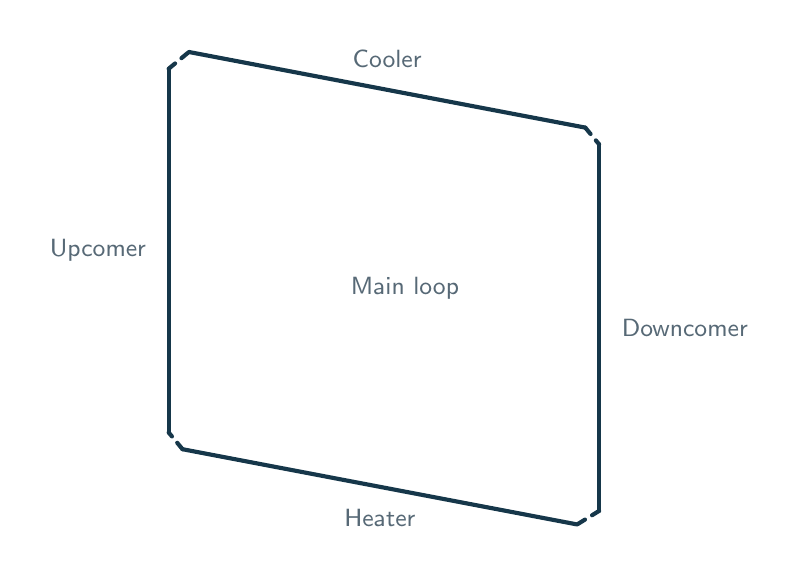
\begin{tikzpicture}[line cap=round,line join=round]
\draw[navy,line width=1.5pt] (0.0000,1.1681) -- (0.0000,5.7873);
\draw[navy,line width=1.5pt,dashed] (0.0000,5.7873) -- (0.2571,6.0000);
\draw[navy,line width=1.5pt] (0.2571,6.0000) -- (5.2908,5.0398);
\draw[navy,line width=1.5pt,dashed] (5.2908,5.0398) -- (5.4668,4.8271);
\draw[navy,line width=1.5pt] (5.4668,4.8271) -- (5.4668,0.1720);
\draw[navy,line width=1.5pt,dashed] (5.4668,0.1720) -- (5.1872,0.0000);
\draw[navy,line width=1.5pt] (5.1872,0.0000) -- (0.1760,0.9554);
\draw[navy,line width=1.5pt,dashed] (0.1760,0.9554) -- (0.0000,1.1681);
\node[font=\small,text=muted,left,inner sep=8pt] at (0.0000,3.4777) {Upcomer};
\node[font=\small,text=muted,above,inner sep=8pt] at (2.7740,5.5199) {Cooler};
\node[font=\small,text=muted,right,inner sep=8pt] at (5.4668,2.4995) {Downcomer};
\node[font=\small,text=muted,below,inner sep=8pt] at (2.6816,0.4777) {Heater};
\node[text=muted,font=\small] at (3,3) {Main loop};
\end{tikzpicture}\par{\footnotesize\color{muted}CAD overview. Dashed corners are schematic.}\end{center}
\vspace{4pt}{\large\bfseries Read the configuration}\par
\hyperref[geometry-main]{Geometry}\quad / \quad\hyperref[insulation-main]{Insulation}\quad / \quad\hyperref[instruments-main]{Instruments}\par
\hyperref[thermal-main]{Heating and cooling}\quad / \quad\hyperref[materials-main]{Materials and fluids}\par
\hyperref[uncertainty-main]{Uncertainty and limitations}\par
\vspace{8pt}\textbf{Adding information?} Open \texttt{VCU\_inputs.xlsx} and start with one Form tab. \hyperref[administration]{Contributor instructions} and \hyperref[appendices]{supporting records} are in the appendices.\par
{\footnotesize\color{muted}Unknown values remain open. This draft records available evidence; it is not a released facility description.}\par
\clearpage\section{Geometry}\label{geometry-main}
Axis-end dimensions and the recorded jacket envelope. Bore and insulation measurements remain open.
\begin{center}\resizebox{0.93\textwidth}{!}{%
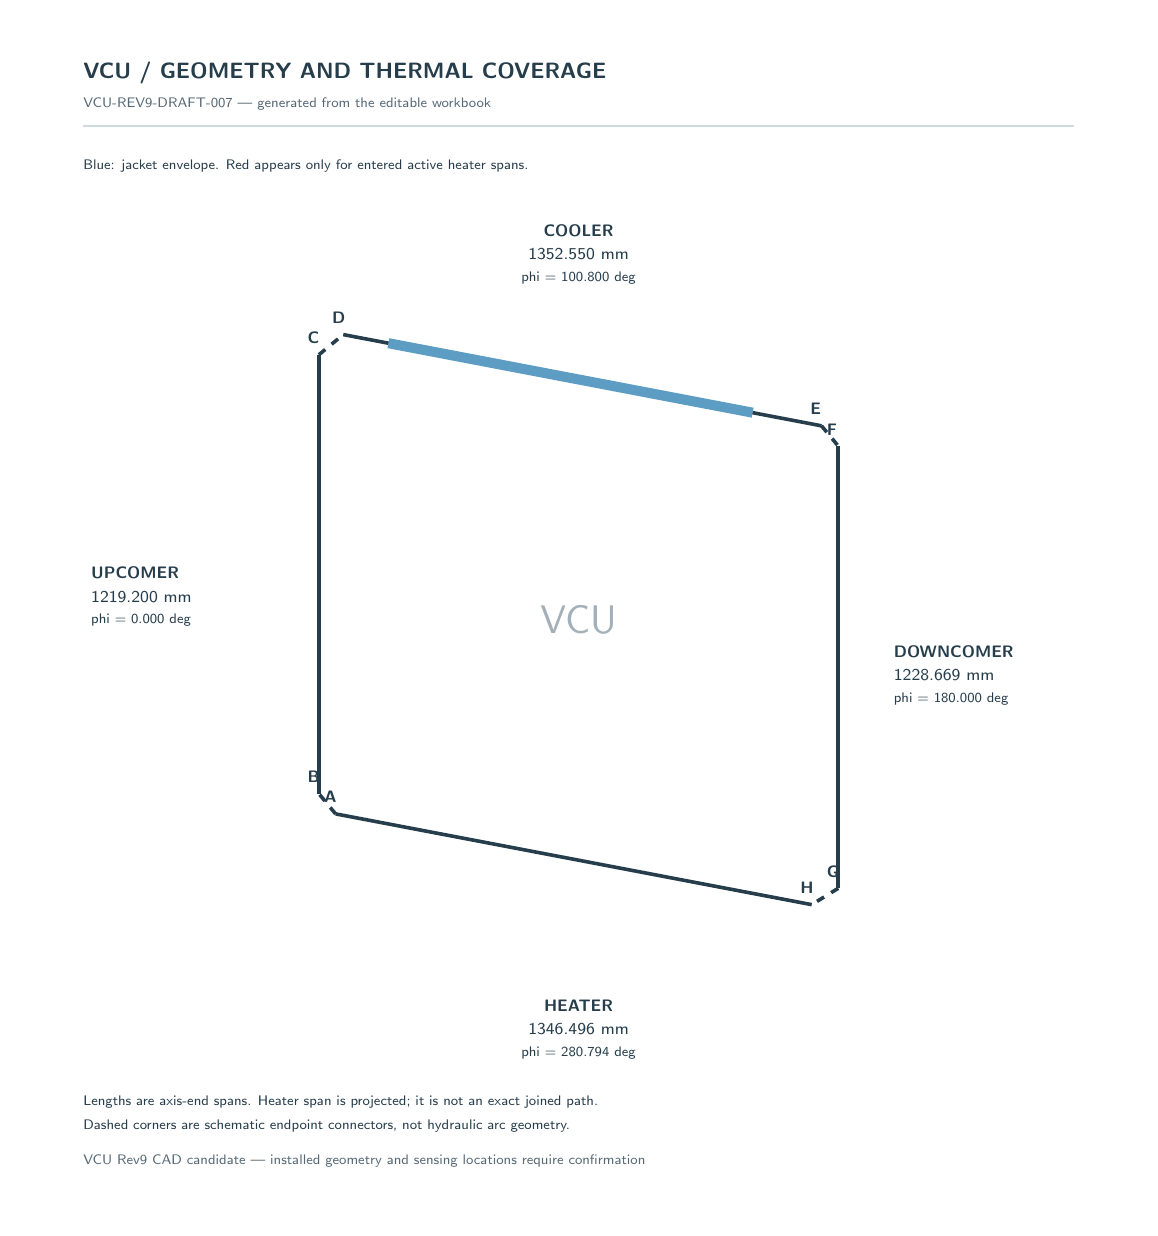
\begin{tikzpicture}[x=0.01cm,y=-0.01cm]
\path[use as bounding box] (0,0) rectangle (1400,1500);
\definecolor{c263D4B}{HTML}{263D4B}
\definecolor{c576976}{HTML}{576976}
\definecolor{c5D9DC3}{HTML}{5D9DC3}
\definecolor{cA3B0B9}{HTML}{A3B0B9}
\definecolor{cCFD9DF}{HTML}{CFD9DF}
\node[anchor=base west,inner sep=0pt,text=c263D4B,font=\sffamily\fontsize{8.40}{10.20}\selectfont\bfseries] at (70.000,65.000) {VCU / GEOMETRY AND THERMAL COVERAGE};
\node[anchor=base west,inner sep=0pt,text=c576976,font=\sffamily\fontsize{4.76}{5.78}\selectfont] at (70.000,102.000) {VCU-REV9-DRAFT-007 | generated from the editable workbook};
\draw[draw=cCFD9DF,line width=0.520pt] (70.000,125.000) -- (1330.000,125.000);
\draw[draw=c263D4B,line width=1.300pt] (370.000,973.358) -- (370.000,415.678);
\draw[draw=c263D4B,line width=1.300pt,dashed] (370.000,415.678) -- (401.040,390.000);
\draw[draw=c263D4B,line width=1.300pt] (401.040,390.000) -- (1008.757,505.928);
\draw[draw=c263D4B,line width=1.300pt,dashed] (1008.757,505.928) -- (1030.000,531.607);
\draw[draw=c263D4B,line width=1.300pt] (1030.000,531.607) -- (1030.000,1093.617);
\draw[draw=c263D4B,line width=1.300pt,dashed] (1030.000,1093.617) -- (996.253,1114.378);
\draw[draw=c263D4B,line width=1.300pt] (996.253,1114.378) -- (391.243,999.036);
\draw[draw=c263D4B,line width=1.300pt,dashed] (391.243,999.036) -- (370.000,973.358);
\draw[draw=c5D9DC3,line width=3.640pt] (458.355,400.933) -- (921.276,489.240);
\node[anchor=base west,inner sep=0pt,text=c263D4B,font=\sffamily\fontsize{5.60}{6.80}\selectfont\bfseries] at (355.000,959.358) {B};
\node[anchor=base west,inner sep=0pt,text=c263D4B,font=\sffamily\fontsize{5.60}{6.80}\selectfont\bfseries] at (355.000,401.678) {C};
\node[anchor=base west,inner sep=0pt,text=c263D4B,font=\sffamily\fontsize{5.60}{6.80}\selectfont\bfseries] at (386.040,376.000) {D};
\node[anchor=base west,inner sep=0pt,text=c263D4B,font=\sffamily\fontsize{5.60}{6.80}\selectfont\bfseries] at (993.757,491.928) {E};
\node[anchor=base west,inner sep=0pt,text=c263D4B,font=\sffamily\fontsize{5.60}{6.80}\selectfont\bfseries] at (1015.000,517.607) {F};
\node[anchor=base west,inner sep=0pt,text=c263D4B,font=\sffamily\fontsize{5.60}{6.80}\selectfont\bfseries] at (1015.000,1079.617) {G};
\node[anchor=base west,inner sep=0pt,text=c263D4B,font=\sffamily\fontsize{5.60}{6.80}\selectfont\bfseries] at (981.253,1100.378) {H};
\node[anchor=base west,inner sep=0pt,text=c263D4B,font=\sffamily\fontsize{5.60}{6.80}\selectfont\bfseries] at (376.243,985.036) {A};
\node[anchor=base,inner sep=0pt,text=cA3B0B9,font=\sffamily\fontsize{15.12}{18.36}\selectfont] at (700.000,770.000) {VCU};
\node[anchor=base west,inner sep=0pt,text=c263D4B,font=\sffamily\fontsize{6.16}{7.48}\selectfont\bfseries] at (80.000,700.000) {UPCOMER};
\node[anchor=base west,inner sep=0pt,text=c263D4B,font=\sffamily\fontsize{5.60}{6.80}\selectfont] at (80.000,730.000) {1219.200 mm};
\node[anchor=base west,inner sep=0pt,text=c263D4B,font=\sffamily\fontsize{4.76}{5.78}\selectfont] at (80.000,757.000) {phi = 0.000 deg};
\node[anchor=base,inner sep=0pt,text=c263D4B,font=\sffamily\fontsize{6.16}{7.48}\selectfont\bfseries] at (700.000,265.000) {COOLER};
\node[anchor=base,inner sep=0pt,text=c263D4B,font=\sffamily\fontsize{5.60}{6.80}\selectfont] at (700.000,295.000) {1352.550 mm};
\node[anchor=base,inner sep=0pt,text=c263D4B,font=\sffamily\fontsize{4.76}{5.78}\selectfont] at (700.000,322.000) {phi = 100.800 deg};
\node[anchor=base west,inner sep=0pt,text=c263D4B,font=\sffamily\fontsize{6.16}{7.48}\selectfont\bfseries] at (1100.000,800.000) {DOWNCOMER};
\node[anchor=base west,inner sep=0pt,text=c263D4B,font=\sffamily\fontsize{5.60}{6.80}\selectfont] at (1100.000,830.000) {1228.669 mm};
\node[anchor=base west,inner sep=0pt,text=c263D4B,font=\sffamily\fontsize{4.76}{5.78}\selectfont] at (1100.000,857.000) {phi = 180.000 deg};
\node[anchor=base,inner sep=0pt,text=c263D4B,font=\sffamily\fontsize{6.16}{7.48}\selectfont\bfseries] at (700.000,1250.000) {HEATER};
\node[anchor=base,inner sep=0pt,text=c263D4B,font=\sffamily\fontsize{5.60}{6.80}\selectfont] at (700.000,1280.000) {1346.496 mm};
\node[anchor=base,inner sep=0pt,text=c263D4B,font=\sffamily\fontsize{4.76}{5.78}\selectfont] at (700.000,1307.000) {phi = 280.794 deg};
\node[anchor=base west,inner sep=0pt,text=c263D4B,font=\sffamily\fontsize{5.04}{6.12}\selectfont] at (70.000,180.000) {Blue: jacket envelope. Red appears only for entered active heater spans.};
\node[anchor=base west,inner sep=0pt,text=c263D4B,font=\sffamily\fontsize{4.76}{5.78}\selectfont] at (70.000,1370.000) {Lengths are axis-end spans. Heater span is projected; it is not an exact joined path.};
\node[anchor=base west,inner sep=0pt,text=c263D4B,font=\sffamily\fontsize{4.76}{5.78}\selectfont] at (70.000,1400.000) {Dashed corners are schematic endpoint connectors, not hydraulic arc geometry.};
\node[anchor=base west,inner sep=0pt,text=c576976,font=\sffamily\fontsize{4.48}{5.44}\selectfont] at (70.000,1445.000) {VCU Rev9 CAD candidate | installed geometry and sensing locations require confirmation};
\end{tikzpicture}
}\end{center}
{\small Details: \hyperref[geometry-detail]{coordinate conventions and CAD qualifications}; \hyperref[baseline-tables]{dimension tables}.}\par
\clearpage\section{Insulation}\label{insulation-main}
Use the workbook\textquotesingle s \textbf{Insulation regions} tab. Every coverage dropdown describes the whole named region.
\begin{center}\resizebox{0.93\textwidth}{!}{%
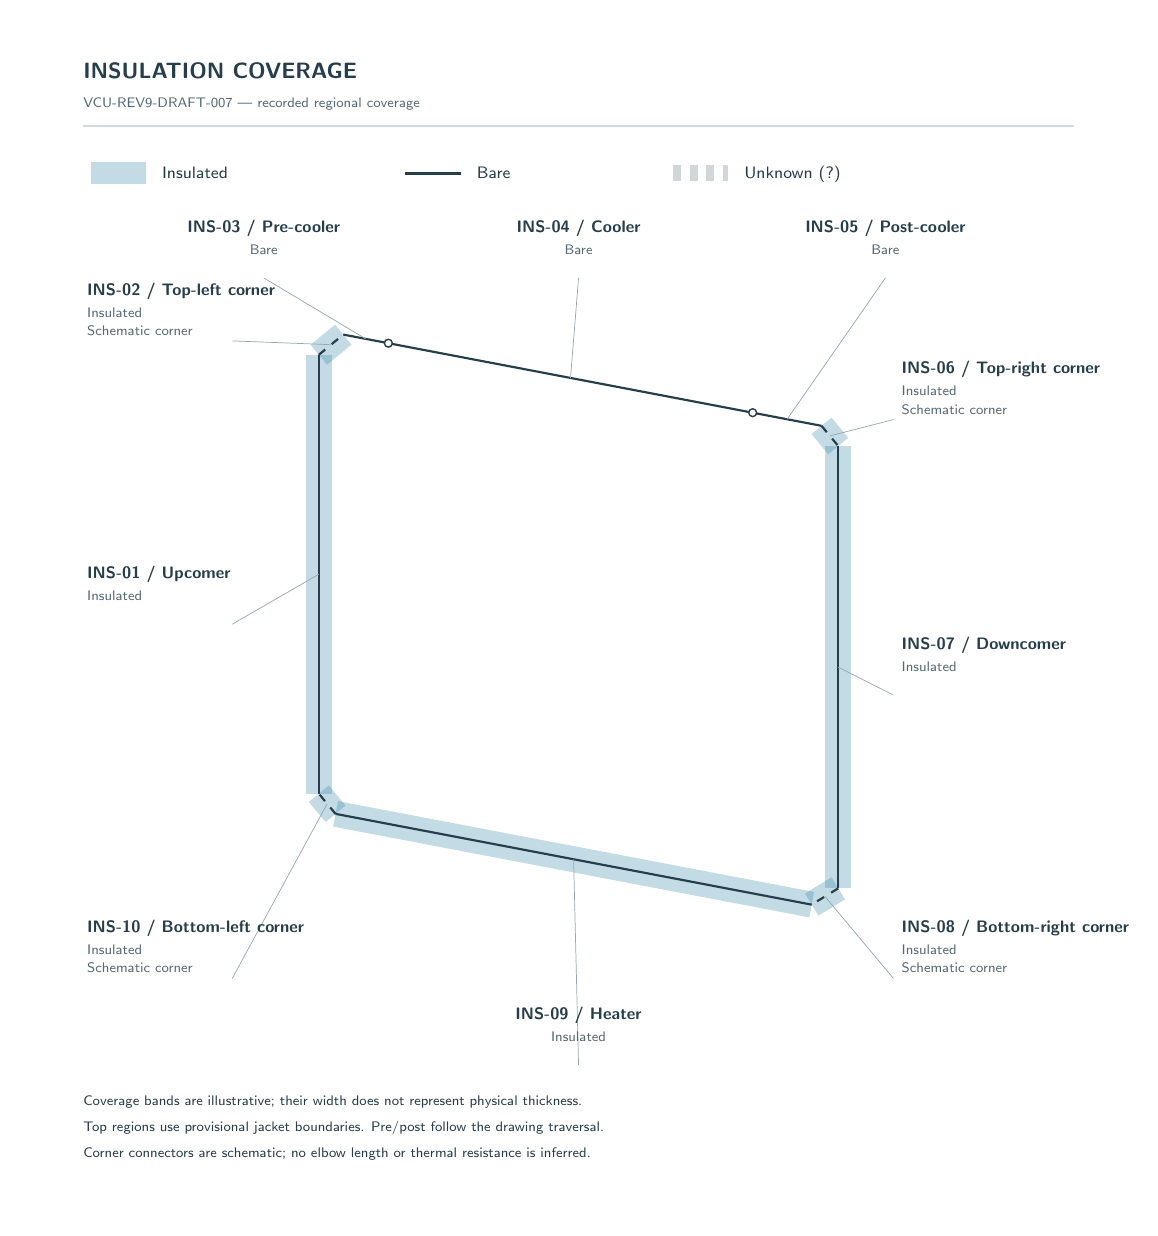
\begin{tikzpicture}[x=0.01cm,y=-0.01cm]
\path[use as bounding box] (0,0) rectangle (1400,1500);
\definecolor{c263D4B}{HTML}{263D4B}
\definecolor{c287FA3}{HTML}{287FA3}
\definecolor{c576976}{HTML}{576976}
\definecolor{c7B8992}{HTML}{7B8992}
\definecolor{c98A7B1}{HTML}{98A7B1}
\definecolor{cCFD9DF}{HTML}{CFD9DF}
\node[anchor=base west,inner sep=0pt,text=c263D4B,font=\sffamily\fontsize{8.40}{10.20}\selectfont\bfseries] at (70.000,65.000) {INSULATION COVERAGE};
\node[anchor=base west,inner sep=0pt,text=c576976,font=\sffamily\fontsize{4.76}{5.78}\selectfont] at (70.000,102.000) {VCU-REV9-DRAFT-007 | recorded regional coverage};
\draw[draw=cCFD9DF,line width=0.520pt] (70.000,125.000) -- (1330.000,125.000);
\draw[draw=c287FA3,line width=7.800pt,draw opacity=0.28] (80.000,185.000) -- (150.000,185.000);
\node[anchor=base west,inner sep=0pt,text=c263D4B,font=\sffamily\fontsize{6.44}{7.82}\selectfont] at (170.000,192.000) {Insulated};
\draw[draw=c263D4B,line width=1.040pt] (480.000,185.000) -- (550.000,185.000);
\node[anchor=base west,inner sep=0pt,text=c263D4B,font=\sffamily\fontsize{6.44}{7.82}\selectfont] at (570.000,192.000) {Bare};
\draw[draw=c7B8992,line width=5.720pt,dashed,draw opacity=0.35] (820.000,185.000) -- (890.000,185.000);
\node[anchor=base west,inner sep=0pt,text=c263D4B,font=\sffamily\fontsize{6.44}{7.82}\selectfont] at (910.000,192.000) {Unknown (?)};
\draw[draw=c287FA3,line width=9.360pt,draw opacity=0.28] (370.000,973.358) -- (370.000,415.678);
\draw[draw=c287FA3,line width=9.360pt,draw opacity=0.28] (370.000,415.678) -- (401.040,390.000);
\draw[draw=c287FA3,line width=9.360pt,draw opacity=0.28] (1008.757,505.928) -- (1030.000,531.607);
\draw[draw=c287FA3,line width=9.360pt,draw opacity=0.28] (1030.000,531.607) -- (1030.000,1093.617);
\draw[draw=c287FA3,line width=9.360pt,draw opacity=0.28] (1030.000,1093.617) -- (996.253,1114.378);
\draw[draw=c287FA3,line width=9.360pt,draw opacity=0.28] (996.253,1114.378) -- (391.243,999.036);
\draw[draw=c287FA3,line width=9.360pt,draw opacity=0.28] (391.243,999.036) -- (370.000,973.358);
\draw[draw=c263D4B,line width=0.780pt] (370.000,973.358) -- (370.000,415.678);
\draw[draw=c263D4B,line width=0.780pt,dashed] (370.000,415.678) -- (401.040,390.000);
\draw[draw=c263D4B,line width=0.780pt] (401.040,390.000) -- (1008.757,505.928);
\draw[draw=c263D4B,line width=0.780pt,dashed] (1008.757,505.928) -- (1030.000,531.607);
\draw[draw=c263D4B,line width=0.780pt] (1030.000,531.607) -- (1030.000,1093.617);
\draw[draw=c263D4B,line width=0.780pt,dashed] (1030.000,1093.617) -- (996.253,1114.378);
\draw[draw=c263D4B,line width=0.780pt] (996.253,1114.378) -- (391.243,999.036);
\draw[draw=c263D4B,line width=0.780pt,dashed] (391.243,999.036) -- (370.000,973.358);
\draw[draw=c98A7B1,line width=0.260pt] (370.000,694.518) -- (260.000,758.000);
\node[anchor=base west,inner sep=0pt,text=c263D4B,font=\sffamily\fontsize{5.60}{6.80}\selectfont\bfseries] at (75.000,700.000) {INS-01 / Upcomer};
\node[anchor=base west,inner sep=0pt,text=c576976,font=\sffamily\fontsize{5.32}{6.46}\selectfont] at (75.000,728.000) {Insulated};
\draw[draw=c98A7B1,line width=0.260pt] (385.520,402.839) -- (260.000,398.000);
\node[anchor=base west,inner sep=0pt,text=c263D4B,font=\sffamily\fontsize{5.60}{6.80}\selectfont\bfseries] at (75.000,340.000) {INS-02 / Top-left corner};
\node[anchor=base west,inner sep=0pt,text=c576976,font=\sffamily\fontsize{5.32}{6.46}\selectfont] at (75.000,368.000) {Insulated};
\node[anchor=base west,inner sep=0pt,text=c576976,font=\sffamily\fontsize{4.48}{5.44}\selectfont] at (75.000,391.000) {Schematic corner};
\draw[draw=c98A7B1,line width=0.260pt] (429.697,395.467) -- (300.000,318.000);
\node[anchor=base,inner sep=0pt,text=c263D4B,font=\sffamily\fontsize{5.60}{6.80}\selectfont\bfseries] at (300.000,260.000) {INS-03 / Pre-cooler};
\node[anchor=base,inner sep=0pt,text=c576976,font=\sffamily\fontsize{5.32}{6.46}\selectfont] at (300.000,288.000) {Bare};
\draw[draw=c98A7B1,line width=0.260pt] (689.815,445.087) -- (700.000,318.000);
\node[anchor=base,inner sep=0pt,text=c263D4B,font=\sffamily\fontsize{5.60}{6.80}\selectfont\bfseries] at (700.000,260.000) {INS-04 / Cooler};
\node[anchor=base,inner sep=0pt,text=c576976,font=\sffamily\fontsize{5.32}{6.46}\selectfont] at (700.000,288.000) {Bare};
\draw[draw=c98A7B1,line width=0.260pt] (965.016,497.584) -- (1090.000,318.000);
\node[anchor=base,inner sep=0pt,text=c263D4B,font=\sffamily\fontsize{5.60}{6.80}\selectfont\bfseries] at (1090.000,260.000) {INS-05 / Post-cooler};
\node[anchor=base,inner sep=0pt,text=c576976,font=\sffamily\fontsize{5.32}{6.46}\selectfont] at (1090.000,288.000) {Bare};
\draw[draw=c98A7B1,line width=0.260pt] (1019.379,518.767) -- (1100.000,498.000);
\node[anchor=base west,inner sep=0pt,text=c263D4B,font=\sffamily\fontsize{5.60}{6.80}\selectfont\bfseries] at (1110.000,440.000) {INS-06 / Top-right corner};
\node[anchor=base west,inner sep=0pt,text=c576976,font=\sffamily\fontsize{5.32}{6.46}\selectfont] at (1110.000,468.000) {Insulated};
\node[anchor=base west,inner sep=0pt,text=c576976,font=\sffamily\fontsize{4.48}{5.44}\selectfont] at (1110.000,491.000) {Schematic corner};
\draw[draw=c98A7B1,line width=0.260pt] (1030.000,812.612) -- (1100.000,848.000);
\node[anchor=base west,inner sep=0pt,text=c263D4B,font=\sffamily\fontsize{5.60}{6.80}\selectfont\bfseries] at (1110.000,790.000) {INS-07 / Downcomer};
\node[anchor=base west,inner sep=0pt,text=c576976,font=\sffamily\fontsize{5.32}{6.46}\selectfont] at (1110.000,818.000) {Insulated};
\draw[draw=c98A7B1,line width=0.260pt] (1013.127,1103.997) -- (1100.000,1208.000);
\node[anchor=base west,inner sep=0pt,text=c263D4B,font=\sffamily\fontsize{5.60}{6.80}\selectfont\bfseries] at (1110.000,1150.000) {INS-08 / Bottom-right corner};
\node[anchor=base west,inner sep=0pt,text=c576976,font=\sffamily\fontsize{5.32}{6.46}\selectfont] at (1110.000,1178.000) {Insulated};
\node[anchor=base west,inner sep=0pt,text=c576976,font=\sffamily\fontsize{4.48}{5.44}\selectfont] at (1110.000,1201.000) {Schematic corner};
\draw[draw=c98A7B1,line width=0.260pt] (693.748,1056.707) -- (700.000,1318.000);
\node[anchor=base,inner sep=0pt,text=c263D4B,font=\sffamily\fontsize{5.60}{6.80}\selectfont\bfseries] at (700.000,1260.000) {INS-09 / Heater};
\node[anchor=base,inner sep=0pt,text=c576976,font=\sffamily\fontsize{5.32}{6.46}\selectfont] at (700.000,1288.000) {Insulated};
\draw[draw=c98A7B1,line width=0.260pt] (380.621,986.197) -- (260.000,1208.000);
\node[anchor=base west,inner sep=0pt,text=c263D4B,font=\sffamily\fontsize{5.60}{6.80}\selectfont\bfseries] at (75.000,1150.000) {INS-10 / Bottom-left corner};
\node[anchor=base west,inner sep=0pt,text=c576976,font=\sffamily\fontsize{5.32}{6.46}\selectfont] at (75.000,1178.000) {Insulated};
\node[anchor=base west,inner sep=0pt,text=c576976,font=\sffamily\fontsize{4.48}{5.44}\selectfont] at (75.000,1201.000) {Schematic corner};
\draw[fill=white,draw=c263D4B,line width=0.5pt] (458.355,400.933) circle (5);
\draw[fill=white,draw=c263D4B,line width=0.5pt] (921.276,489.240) circle (5);
\node[anchor=base west,inner sep=0pt,text=c263D4B,font=\sffamily\fontsize{5.04}{6.12}\selectfont] at (70.000,1370.000) {Coverage bands are illustrative; their width does not represent physical thickness.};
\node[anchor=base west,inner sep=0pt,text=c263D4B,font=\sffamily\fontsize{5.04}{6.12}\selectfont] at (70.000,1403.000) {Top regions use provisional jacket boundaries. Pre/post follow the drawing traversal.};
\node[anchor=base west,inner sep=0pt,text=c263D4B,font=\sffamily\fontsize{5.04}{6.12}\selectfont] at (70.000,1436.000) {Corner connectors are schematic; no elbow length or thermal resistance is inferred.};
\end{tikzpicture}
}\end{center}
{\small Details: \hyperref[insulation-detail]{materials, thickness and evidence by region}. No resistance factors or boundary conditions are calculated.}\par
\clearpage\section{Instruments}\label{instruments-main}
Geometric sensor references on the main loop. Working native-channel bindings are documented separately; installed junctions and calibration still require evidence.
\begin{center}\resizebox{0.93\textwidth}{!}{%
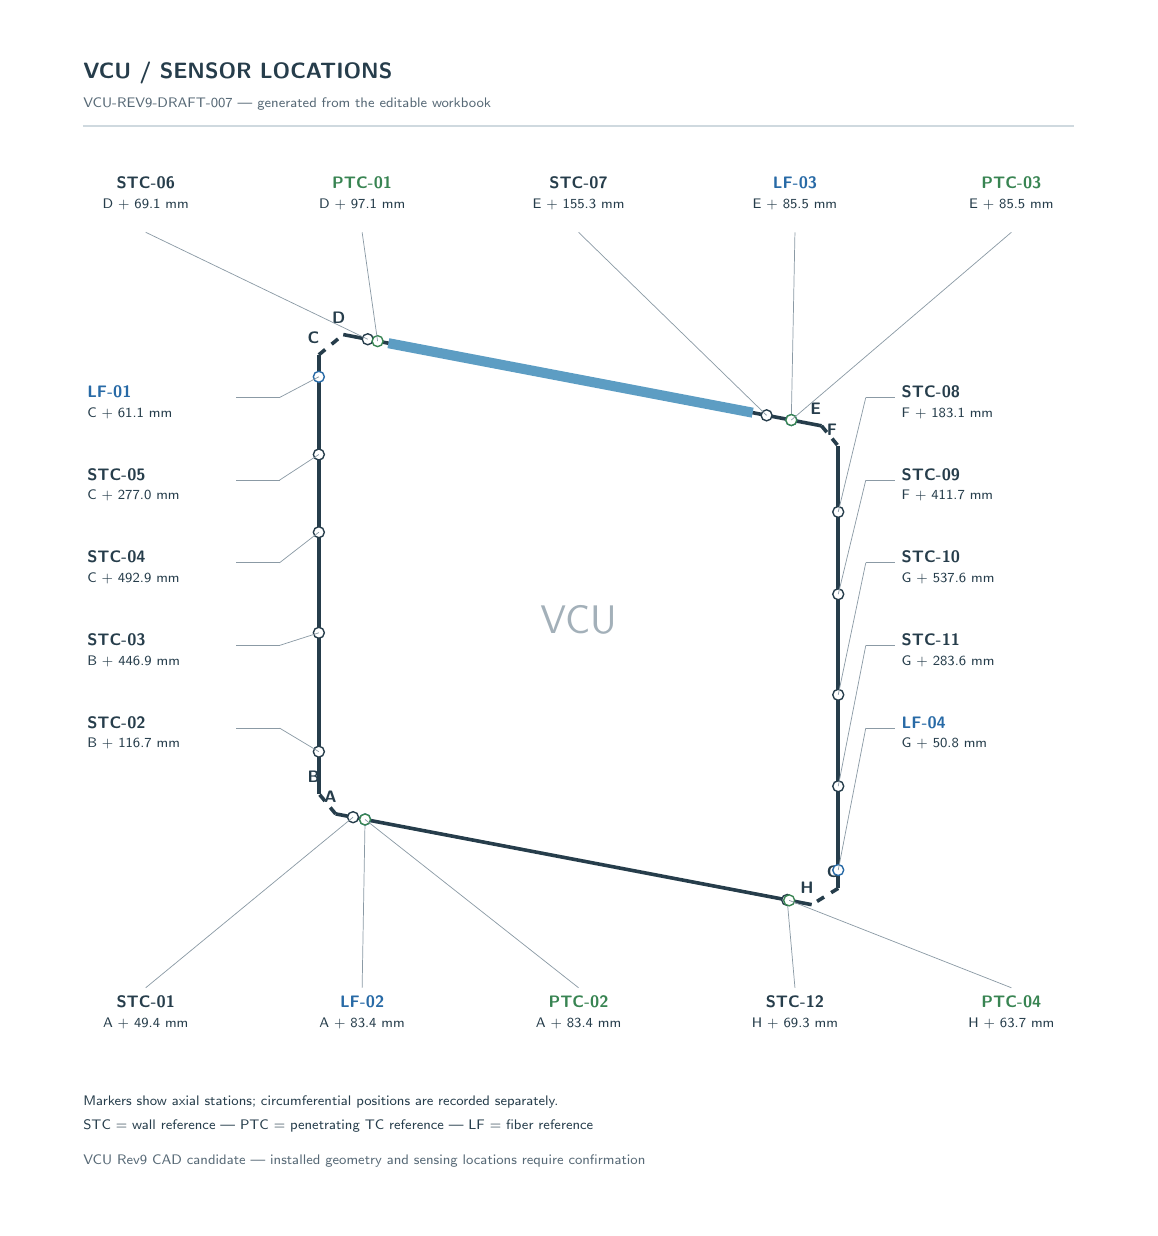
\begin{tikzpicture}[x=0.01cm,y=-0.01cm]
\path[use as bounding box] (0,0) rectangle (1400,1500);
\definecolor{c263D4B}{HTML}{263D4B}
\definecolor{c286AA6}{HTML}{286AA6}
\definecolor{c388452}{HTML}{388452}
\definecolor{c576976}{HTML}{576976}
\definecolor{c5D9DC3}{HTML}{5D9DC3}
\definecolor{c8B9AA5}{HTML}{8B9AA5}
\definecolor{cA3B0B9}{HTML}{A3B0B9}
\definecolor{cCFD9DF}{HTML}{CFD9DF}
\node[anchor=base west,inner sep=0pt,text=c263D4B,font=\sffamily\fontsize{8.40}{10.20}\selectfont\bfseries] at (70.000,65.000) {VCU / SENSOR LOCATIONS};
\node[anchor=base west,inner sep=0pt,text=c576976,font=\sffamily\fontsize{4.76}{5.78}\selectfont] at (70.000,102.000) {VCU-REV9-DRAFT-007 | generated from the editable workbook};
\draw[draw=cCFD9DF,line width=0.520pt] (70.000,125.000) -- (1330.000,125.000);
\draw[draw=c263D4B,line width=1.300pt] (370.000,973.358) -- (370.000,415.678);
\draw[draw=c263D4B,line width=1.300pt,dashed] (370.000,415.678) -- (401.040,390.000);
\draw[draw=c263D4B,line width=1.300pt] (401.040,390.000) -- (1008.757,505.928);
\draw[draw=c263D4B,line width=1.300pt,dashed] (1008.757,505.928) -- (1030.000,531.607);
\draw[draw=c263D4B,line width=1.300pt] (1030.000,531.607) -- (1030.000,1093.617);
\draw[draw=c263D4B,line width=1.300pt,dashed] (1030.000,1093.617) -- (996.253,1114.378);
\draw[draw=c263D4B,line width=1.300pt] (996.253,1114.378) -- (391.243,999.036);
\draw[draw=c263D4B,line width=1.300pt,dashed] (391.243,999.036) -- (370.000,973.358);
\draw[draw=c5D9DC3,line width=3.640pt] (458.355,400.933) -- (921.276,489.240);
\node[anchor=base west,inner sep=0pt,text=c263D4B,font=\sffamily\fontsize{5.60}{6.80}\selectfont\bfseries] at (355.000,959.358) {B};
\node[anchor=base west,inner sep=0pt,text=c263D4B,font=\sffamily\fontsize{5.60}{6.80}\selectfont\bfseries] at (355.000,401.678) {C};
\node[anchor=base west,inner sep=0pt,text=c263D4B,font=\sffamily\fontsize{5.60}{6.80}\selectfont\bfseries] at (386.040,376.000) {D};
\node[anchor=base west,inner sep=0pt,text=c263D4B,font=\sffamily\fontsize{5.60}{6.80}\selectfont\bfseries] at (993.757,491.928) {E};
\node[anchor=base west,inner sep=0pt,text=c263D4B,font=\sffamily\fontsize{5.60}{6.80}\selectfont\bfseries] at (1015.000,517.607) {F};
\node[anchor=base west,inner sep=0pt,text=c263D4B,font=\sffamily\fontsize{5.60}{6.80}\selectfont\bfseries] at (1015.000,1079.617) {G};
\node[anchor=base west,inner sep=0pt,text=c263D4B,font=\sffamily\fontsize{5.60}{6.80}\selectfont\bfseries] at (981.253,1100.378) {H};
\node[anchor=base west,inner sep=0pt,text=c263D4B,font=\sffamily\fontsize{5.60}{6.80}\selectfont\bfseries] at (376.243,985.036) {A};
\node[anchor=base,inner sep=0pt,text=cA3B0B9,font=\sffamily\fontsize{15.12}{18.36}\selectfont] at (700.000,770.000) {VCU};
\draw[fill=white,draw=c286AA6,line width=0.5pt] (370.000,443.633) circle (7);
\draw[draw=c8B9AA5,line width=0.260pt] (370.000,443.633) -- (320.000,470.000);
\draw[draw=c8B9AA5,line width=0.260pt] (320.000,470.000) -- (265.000,470.000);
\node[anchor=base west,inner sep=0pt,text=c286AA6,font=\sffamily\fontsize{5.60}{6.80}\selectfont\bfseries] at (75.000,470.000) {LF-01};
\node[anchor=base west,inner sep=0pt,text=c263D4B,font=\sffamily\fontsize{4.48}{5.44}\selectfont] at (75.000,495.000) {C + 61.1 mm};
\draw[fill=white,draw=c263D4B,line width=0.5pt] (370.000,542.388) circle (7);
\draw[draw=c8B9AA5,line width=0.260pt] (370.000,542.388) -- (320.000,575.000);
\draw[draw=c8B9AA5,line width=0.260pt] (320.000,575.000) -- (265.000,575.000);
\node[anchor=base west,inner sep=0pt,text=c263D4B,font=\sffamily\fontsize{5.60}{6.80}\selectfont\bfseries] at (75.000,575.000) {STC-05};
\node[anchor=base west,inner sep=0pt,text=c263D4B,font=\sffamily\fontsize{4.48}{5.44}\selectfont] at (75.000,600.000) {C + 277.0 mm};
\draw[fill=white,draw=c263D4B,line width=0.5pt] (370.000,641.144) circle (7);
\draw[draw=c8B9AA5,line width=0.260pt] (370.000,641.144) -- (320.000,680.000);
\draw[draw=c8B9AA5,line width=0.260pt] (320.000,680.000) -- (265.000,680.000);
\node[anchor=base west,inner sep=0pt,text=c263D4B,font=\sffamily\fontsize{5.60}{6.80}\selectfont\bfseries] at (75.000,680.000) {STC-04};
\node[anchor=base west,inner sep=0pt,text=c263D4B,font=\sffamily\fontsize{4.48}{5.44}\selectfont] at (75.000,705.000) {C + 492.9 mm};
\draw[fill=white,draw=c263D4B,line width=0.5pt] (370.000,768.946) circle (7);
\draw[draw=c8B9AA5,line width=0.260pt] (370.000,768.946) -- (320.000,785.000);
\draw[draw=c8B9AA5,line width=0.260pt] (320.000,785.000) -- (265.000,785.000);
\node[anchor=base west,inner sep=0pt,text=c263D4B,font=\sffamily\fontsize{5.60}{6.80}\selectfont\bfseries] at (75.000,785.000) {STC-03};
\node[anchor=base west,inner sep=0pt,text=c263D4B,font=\sffamily\fontsize{4.48}{5.44}\selectfont] at (75.000,810.000) {B + 446.9 mm};
\draw[fill=white,draw=c263D4B,line width=0.5pt] (370.000,919.984) circle (7);
\draw[draw=c8B9AA5,line width=0.260pt] (370.000,919.984) -- (320.000,890.000);
\draw[draw=c8B9AA5,line width=0.260pt] (320.000,890.000) -- (265.000,890.000);
\node[anchor=base west,inner sep=0pt,text=c263D4B,font=\sffamily\fontsize{5.60}{6.80}\selectfont\bfseries] at (75.000,890.000) {STC-02};
\node[anchor=base west,inner sep=0pt,text=c263D4B,font=\sffamily\fontsize{4.48}{5.44}\selectfont] at (75.000,915.000) {B + 116.7 mm};
\draw[fill=white,draw=c263D4B,line width=0.5pt] (432.106,395.926) circle (7);
\draw[draw=c8B9AA5,line width=0.260pt] (432.106,395.926) -- (150.000,260.000);
\node[anchor=base,inner sep=0pt,text=c263D4B,font=\sffamily\fontsize{5.60}{6.80}\selectfont\bfseries] at (150.000,205.000) {STC-06};
\node[anchor=base,inner sep=0pt,text=c263D4B,font=\sffamily\fontsize{4.48}{5.44}\selectfont] at (150.000,230.000) {D + 69.1 mm};
\draw[fill=white,draw=c388452,line width=0.5pt] (444.659,398.321) circle (7);
\draw[draw=c8B9AA5,line width=0.260pt] (444.659,398.321) -- (425.000,260.000);
\node[anchor=base,inner sep=0pt,text=c388452,font=\sffamily\fontsize{5.60}{6.80}\selectfont\bfseries] at (425.000,205.000) {PTC-01};
\node[anchor=base,inner sep=0pt,text=c263D4B,font=\sffamily\fontsize{4.48}{5.44}\selectfont] at (425.000,230.000) {D + 97.1 mm};
\draw[fill=white,draw=c263D4B,line width=0.5pt] (938.965,492.615) circle (7);
\draw[draw=c8B9AA5,line width=0.260pt] (938.965,492.615) -- (700.000,260.000);
\node[anchor=base,inner sep=0pt,text=c263D4B,font=\sffamily\fontsize{5.60}{6.80}\selectfont\bfseries] at (700.000,205.000) {STC-07};
\node[anchor=base,inner sep=0pt,text=c263D4B,font=\sffamily\fontsize{4.48}{5.44}\selectfont] at (700.000,230.000) {E + 155.3 mm};
\draw[fill=white,draw=c286AA6,line width=0.5pt] (970.350,498.602) circle (7);
\draw[draw=c8B9AA5,line width=0.260pt] (970.350,498.602) -- (975.000,260.000);
\node[anchor=base,inner sep=0pt,text=c286AA6,font=\sffamily\fontsize{5.60}{6.80}\selectfont\bfseries] at (975.000,205.000) {LF-03};
\node[anchor=base,inner sep=0pt,text=c263D4B,font=\sffamily\fontsize{4.48}{5.44}\selectfont] at (975.000,230.000) {E + 85.5 mm};
\draw[fill=white,draw=c388452,line width=0.5pt] (970.350,498.602) circle (7);
\draw[draw=c8B9AA5,line width=0.260pt] (970.350,498.602) -- (1250.000,260.000);
\node[anchor=base,inner sep=0pt,text=c388452,font=\sffamily\fontsize{5.60}{6.80}\selectfont\bfseries] at (1250.000,205.000) {PTC-03};
\node[anchor=base,inner sep=0pt,text=c263D4B,font=\sffamily\fontsize{4.48}{5.44}\selectfont] at (1250.000,230.000) {E + 85.5 mm};
\draw[fill=white,draw=c263D4B,line width=0.5pt] (1030.000,615.361) circle (7);
\draw[draw=c8B9AA5,line width=0.260pt] (1030.000,615.361) -- (1065.000,470.000);
\draw[draw=c8B9AA5,line width=0.260pt] (1065.000,470.000) -- (1102.000,470.000);
\node[anchor=base west,inner sep=0pt,text=c263D4B,font=\sffamily\fontsize{5.60}{6.80}\selectfont\bfseries] at (1110.000,470.000) {STC-08};
\node[anchor=base west,inner sep=0pt,text=c263D4B,font=\sffamily\fontsize{4.48}{5.44}\selectfont] at (1110.000,495.000) {F + 183.1 mm};
\draw[fill=white,draw=c263D4B,line width=0.5pt] (1030.000,719.926) circle (7);
\draw[draw=c8B9AA5,line width=0.260pt] (1030.000,719.926) -- (1065.000,575.000);
\draw[draw=c8B9AA5,line width=0.260pt] (1065.000,575.000) -- (1102.000,575.000);
\node[anchor=base west,inner sep=0pt,text=c263D4B,font=\sffamily\fontsize{5.60}{6.80}\selectfont\bfseries] at (1110.000,575.000) {STC-09};
\node[anchor=base west,inner sep=0pt,text=c263D4B,font=\sffamily\fontsize{4.48}{5.44}\selectfont] at (1110.000,600.000) {F + 411.7 mm};
\draw[fill=white,draw=c263D4B,line width=0.5pt] (1030.000,847.728) circle (7);
\draw[draw=c8B9AA5,line width=0.260pt] (1030.000,847.728) -- (1065.000,680.000);
\draw[draw=c8B9AA5,line width=0.260pt] (1065.000,680.000) -- (1102.000,680.000);
\node[anchor=base west,inner sep=0pt,text=c263D4B,font=\sffamily\fontsize{5.60}{6.80}\selectfont\bfseries] at (1110.000,680.000) {STC-10};
\node[anchor=base west,inner sep=0pt,text=c263D4B,font=\sffamily\fontsize{4.48}{5.44}\selectfont] at (1110.000,705.000) {G + 537.6 mm};
\draw[fill=white,draw=c263D4B,line width=0.5pt] (1030.000,963.911) circle (7);
\draw[draw=c8B9AA5,line width=0.260pt] (1030.000,963.911) -- (1065.000,785.000);
\draw[draw=c8B9AA5,line width=0.260pt] (1065.000,785.000) -- (1102.000,785.000);
\node[anchor=base west,inner sep=0pt,text=c263D4B,font=\sffamily\fontsize{5.60}{6.80}\selectfont\bfseries] at (1110.000,785.000) {STC-11};
\node[anchor=base west,inner sep=0pt,text=c263D4B,font=\sffamily\fontsize{4.48}{5.44}\selectfont] at (1110.000,810.000) {G + 283.6 mm};
\draw[fill=white,draw=c286AA6,line width=0.5pt] (1030.000,1070.381) circle (7);
\draw[draw=c8B9AA5,line width=0.260pt] (1030.000,1070.381) -- (1065.000,890.000);
\draw[draw=c8B9AA5,line width=0.260pt] (1065.000,890.000) -- (1102.000,890.000);
\node[anchor=base west,inner sep=0pt,text=c286AA6,font=\sffamily\fontsize{5.60}{6.80}\selectfont\bfseries] at (1110.000,890.000) {LF-04};
\node[anchor=base west,inner sep=0pt,text=c263D4B,font=\sffamily\fontsize{4.48}{5.44}\selectfont] at (1110.000,915.000) {G + 50.8 mm};
\draw[fill=white,draw=c263D4B,line width=0.5pt] (413.452,1003.270) circle (7);
\draw[draw=c8B9AA5,line width=0.260pt] (413.452,1003.270) -- (150.000,1220.000);
\node[anchor=base,inner sep=0pt,text=c263D4B,font=\sffamily\fontsize{5.60}{6.80}\selectfont\bfseries] at (150.000,1245.000) {STC-01};
\node[anchor=base,inner sep=0pt,text=c263D4B,font=\sffamily\fontsize{4.48}{5.44}\selectfont] at (150.000,1270.000) {A + 49.4 mm};
\draw[fill=white,draw=c286AA6,line width=0.5pt] (428.714,1006.180) circle (7);
\draw[draw=c8B9AA5,line width=0.260pt] (428.714,1006.180) -- (425.000,1220.000);
\node[anchor=base,inner sep=0pt,text=c286AA6,font=\sffamily\fontsize{5.60}{6.80}\selectfont\bfseries] at (425.000,1245.000) {LF-02};
\node[anchor=base,inner sep=0pt,text=c263D4B,font=\sffamily\fontsize{4.48}{5.44}\selectfont] at (425.000,1270.000) {A + 83.4 mm};
\draw[fill=white,draw=c388452,line width=0.5pt] (428.714,1006.180) circle (7);
\draw[draw=c8B9AA5,line width=0.260pt] (428.714,1006.180) -- (700.000,1220.000);
\node[anchor=base,inner sep=0pt,text=c388452,font=\sffamily\fontsize{5.60}{6.80}\selectfont\bfseries] at (700.000,1245.000) {PTC-02};
\node[anchor=base,inner sep=0pt,text=c263D4B,font=\sffamily\fontsize{4.48}{5.44}\selectfont] at (700.000,1270.000) {A + 83.4 mm};
\draw[fill=white,draw=c263D4B,line width=0.5pt] (965.118,1108.442) circle (7);
\draw[draw=c8B9AA5,line width=0.260pt] (965.118,1108.442) -- (975.000,1220.000);
\node[anchor=base,inner sep=0pt,text=c263D4B,font=\sffamily\fontsize{5.60}{6.80}\selectfont\bfseries] at (975.000,1245.000) {STC-12};
\node[anchor=base,inner sep=0pt,text=c263D4B,font=\sffamily\fontsize{4.48}{5.44}\selectfont] at (975.000,1270.000) {H + 69.3 mm};
\draw[fill=white,draw=c388452,line width=0.5pt] (967.624,1108.920) circle (7);
\draw[draw=c8B9AA5,line width=0.260pt] (967.624,1108.920) -- (1250.000,1220.000);
\node[anchor=base,inner sep=0pt,text=c388452,font=\sffamily\fontsize{5.60}{6.80}\selectfont\bfseries] at (1250.000,1245.000) {PTC-04};
\node[anchor=base,inner sep=0pt,text=c263D4B,font=\sffamily\fontsize{4.48}{5.44}\selectfont] at (1250.000,1270.000) {H + 63.7 mm};
\node[anchor=base west,inner sep=0pt,text=c263D4B,font=\sffamily\fontsize{4.76}{5.78}\selectfont] at (70.000,1370.000) {Markers show axial stations; circumferential positions are recorded separately.};
\node[anchor=base west,inner sep=0pt,text=c263D4B,font=\sffamily\fontsize{4.76}{5.78}\selectfont] at (70.000,1400.000) {STC = wall reference | PTC = penetrating TC reference | LF = fiber reference};
\node[anchor=base west,inner sep=0pt,text=c576976,font=\sffamily\fontsize{4.48}{5.44}\selectfont] at (70.000,1445.000) {VCU Rev9 CAD candidate | installed geometry and sensing locations require confirmation};
\end{tikzpicture}
}\end{center}
{\small Details: \hyperref[calibration-detail]{calibration and model mapping}; \hyperref[form-sensor]{sensor evidence form}. Jacket-port sensors JTC-A/B are retained in the calibration record.}\par
\clearpage\section{Heating and cooling}\label{thermal-main}
The mechanical jacket envelope and active thermal regions are recorded separately.
\subsection*{Recorded boundaries}
\par
\small\setlength{\tabcolsep}{4pt}
\begin{longtable}{>{\raggedright\arraybackslash}p{0.22\textwidth}>{\raggedright\arraybackslash}p{0.2\textwidth}>{\raggedright\arraybackslash}p{0.14\textwidth}>{\raggedright\arraybackslash}p{0.14\textwidth}>{\raggedright\arraybackslash}p{0.2\textwidth}}
\toprule
\textbf{Region} & \textbf{Segment / from} & \textbf{Start mm} & \textbf{End mm} & \textbf{Basis} \\\midrule\endhead
Complete jacket & cooler / D & 127.562 & 1157.849 & CAD-derived \\[3pt]
Active heater & heater / H & \textit{Unknown} & \textit{Unknown} & Unknown \\[3pt]
Active cooling & cooler / D & \textit{Unknown} & \textit{Unknown} & Unknown \\[3pt]
\bottomrule\end{longtable}\normalsize
Distances are measured along the named segment from the stated endpoint. A jacket envelope does not establish active cooling; clamps do not establish energized heater coverage.\par
\subsection*{Power and control evidence}
\small\setlength{\tabcolsep}{4pt}
\begin{longtable}{>{\raggedright\arraybackslash}p{0.43\textwidth}>{\raggedright\arraybackslash}p{0.24\textwidth}>{\raggedright\arraybackslash}p{0.23\textwidth}}
\toprule
\textbf{Record} & \textbf{Selected choice} & \textbf{Review} \\\midrule\endhead
Heater supply and circuit diagram & Not selected & Needs review \\[3pt]
Measured heater power and uncertainty & Not selected & Needs information \\[3pt]
Heater control and monitor signals & Not selected & Needs information \\[3pt]
Coolant routing and measurement planes & JTC-B/PTC5 inlet; JTC-A/PTC6 outlet & Needs review \\[3pt]
Coolant flow and inlet/outlet measurements & Use temperature roles provisionally; do not invent flow or measured duty & Needs review \\[3pt]
Cooler feedback and setpoint history & Treat oscillatory plateaus as potentially cyclic operation & Needs review \\[3pt]
\bottomrule\end{longtable}\normalsize
\vfill{\small Supporting records: \hyperref[model-records]{boundary and control choices}; \hyperref[requirements]{decisions and evidence}.}\par
\clearpage\section{Materials and fluids}\label{materials-main}
Candidate identities are listed below. Circuit assignments and selected property models require their own evidence.
\subsection*{Fluids}
\small\setlength{\tabcolsep}{4pt}
\begin{longtable}{>{\raggedright\arraybackslash}p{0.15\textwidth}>{\raggedright\arraybackslash}p{0.39\textwidth}>{\raggedright\arraybackslash}p{0.18\textwidth}>{\raggedright\arraybackslash}p{0.18\textwidth}}
\toprule
\textbf{Fluid} & \textbf{Product} & \textbf{Circuit} & \textbf{Basis} \\\midrule\endhead
PROP30 & Propylene glycol / water & Primary-loop candidate; select per run & Reported \\[3pt]
AIR & Air & Primary-loop option and room ambient; distinguish per run & Reported \\[3pt]
WATER & Water & Reported jacket coolant; primary-loop option per run & Reported \\[3pt]
\bottomrule\end{longtable}\normalsize
\subsection*{Material and property records}
\small\setlength{\tabcolsep}{4pt}
\begin{longtable}{>{\raggedright\arraybackslash}p{0.18\textwidth}>{\raggedright\arraybackslash}p{0.53\textwidth}>{\raggedright\arraybackslash}p{0.19\textwidth}}
\toprule
\textbf{Record} & \textbf{Identity / product} & \textbf{Basis} \\\midrule\endhead
PIPE & 316L stainless steel & Reported \\[3pt]
MAIN-INS & Fiberglass / reported McMaster 5556K73 & Reported \\[3pt]
HEATER-INS & Calcium aluminum silicate / reported 4057K14 & Reported \\[3pt]
PROP30 & Product/formulation unresolved & Reported \\[3pt]
AIR & Air & Unknown \\[3pt]
WATER & Water & Unknown \\[3pt]
\bottomrule\end{longtable}\normalsize
\vfill{\small Property applicability and model choices: \hyperref[model-records]{technical records}. To propose a property choice: \hyperref[form-material]{material evidence form}. Full equations and units remain in the workbook and detailed audit.}\par
\clearpage\section{Uncertainty and limitations}\label{uncertainty-main}
The record must state how accurately the setup is known and what error is acceptable for each intended comparison.
\small\setlength{\tabcolsep}{4pt}
\begin{longtable}{>{\raggedright\arraybackslash}p{0.43\textwidth}>{\raggedright\arraybackslash}p{0.24\textwidth}>{\raggedright\arraybackslash}p{0.23\textwidth}}
\toprule
\textbf{Basis for comparison} & \textbf{Selected choice} & \textbf{Review} \\\midrule\endhead
Dimension uncertainty and method & Not selected & Needs information \\[3pt]
Measurement uncertainty and coverage & Not selected & Needs information \\[3pt]
Property uncertainty and fit residuals & Not selected & Needs information \\[3pt]
Steady-state class and acceptance limits & Keep exploratory classifications separate from accepted steady-state limits & Needs review \\[3pt]
Mass/energy conservation and solution convergence & Not selected & Needs information \\[3pt]
Validation metrics, discrepancy and applicability & Retain conservation/uncertainty checks and predeclared unseen assessment & Needs review \\[3pt]
\bottomrule\end{longtable}\normalsize
\subsection*{Limits of this record}
\begin{itemize}\item The main-loop geometry is a CAD candidate. Installed dimensions, bore and insulation need supporting measurements.\item Sensor stations are geometric references. Channel identity, calibration, junction positions and fiber sensing extents require evidence.\item Drawn bends are schematic connectors, not qualified hydraulic paths. The heater pieces have overlapping and offset CAD geometry.\item A successful document build checks input structure and drawing closure. It does not establish experimental or modeling readiness.\end{itemize}
\vfill{\small Follow up: \hyperref[issues-detail]{open issues}; \hyperref[requirements]{requirements and decisions}; \hyperref[sources-detail]{source catalog}.}\par
\clearpage\phantomsection\label{appendices}\pdfbookmark[0]{Appendices}{appendix-bookmark}
{\color{navy}\LARGE\bfseries Appendices}\par
Instructions, evidence and administrative detail. Return to the \hyperref[overview]{configuration overview} at any time using the page header.\par
\tableofcontents
\appendix
\clearpage\section{Contributing evidence and reviewing changes}\label{administration}
\section*{Start with one record}
You do not need to learn LaTeX to contribute. Open \textbf{VCU\_inputs.xlsx}, choose a Form tab, and fill the amber response cells. The package maintainer turns the saved workbook into this document and the labeled drawings.
\begin{enumerate}
\item \textbf{Choose one item.} Start with the upcomer pipe, the STC-02 sensor reference, or the insulation conductivity example.
\item \textbf{Read the reference.} Gray cells show what the supplied evidence says and where to find it. They are not confirmed answers.
\item \textbf{Enter what you know.} Add units, measurement date and the point or component you checked. Leave unknown values blank; add the open question in the evidence cell.
\item \textbf{Attach proof.} Name the file and the exact photo, page, row or certificate. Choose the evidence type and add your name/date.
\item \textbf{Return it for review.} The reviewer records the decision and its scope. Form entries do not automatically replace the baseline.
\end{enumerate}
\textbf{A useful first return:} one completed form, its evidence files, and a short list of anything you could not confirm. A partial, honest record is useful.
\textbf{Keep the example attached to its item.} To work on a different segment, sensor or material, save a separate response copy. Clear the old example references or have the maintainer replace them with evidence for the new item.
\textbf{Find your page:} pipe form p.~\pageref{form-pipe}; sensor form p.~\pageref{form-sensor}; property form p.~\pageref{form-material}; phase requests p.~\pageref{phase-requests}; complete requirements p.~\pageref{requirements}.
\textbf{Need help?} The repository file \textbf{support/docs/START\_HERE.md} has separate paths for the experimental team, computational team and package maintainer.
\clearpage\section{Who fills in what?}
\textbf{Experimental team.} Record the installed hardware, fluids, sensor/channel mapping, calibration evidence, electrical wiring, coolant routing and raw logs. Use the phase requests to see what evidence is needed next.
\textbf{Computational team.} Propose model domains, boundary conditions, material correlations, uncertainty methods and validation checks. Explain the intended use and why each choice is suitable.
\textbf{Package reviewer.} Resolve conflicting evidence and record the approved choice, scope, date and effective configuration. The listed teams are suggested owners; named owners and release authority still need confirmation.
\textbf{Package maintainer.} Preserve the submitted evidence, update accepted input records deliberately, regenerate, and check that the document and diagrams match the saved workbook.
\subsection*{Two labels answer two different questions}
\small\setlength{\tabcolsep}{4pt}
\begin{longtable}{>{\raggedright\arraybackslash}p{0.24\textwidth}>{\raggedright\arraybackslash}p{0.68\textwidth}}
\toprule
\textbf{Evidence type} & \textbf{What it means} \\\midrule\endhead
CAD-derived & A result from the identified Rev9 model; installation not verified. \\[3pt]
Installed measurement & A measured physical item with date, method and evidence. \\[3pt]
Reported & A statement in notes or a communication; original evidence may still be needed. \\[3pt]
Modeling assumption & A proposed idealization or convention requiring rationale. \\[3pt]
Unknown & No supported value is available yet. \\[3pt]
\bottomrule\end{longtable}\normalsize
\textbf{Review state is separate:} Needs information, Needs review, Approved for stated use, or Not applicable with a reason. Approval must name the selected value, reviewer, date and scope. A CAD-derived value stays CAD-derived after review. Working selections are recorded with their scope and source; package release and installed verification remain pending.
\subsection*{What belongs in each package?}
\textbf{Configuration Control} describes the physical setup and measurement chain: geometry, insulation, fluids, instruments, calibration, heating/cooling, branch states and run identity.
\textbf{Modeling Control} describes how that setup is represented: 1-D and CFD/CHT domains, boundary/initial conditions, shared properties, closures, numerical checks, uncertainty and independent validation.
\textbf{Shared records} connect the two: evidence, approvals, sensor-to-model mapping, measured power, property selection and validation applicability.
\notebox{The STNCL documents are draft evidence sources. The requests in this package do not authorize running a test or establish that Nick Luciano has approved the draft requirements.}
\par
\clearpage\section{Configuration record and acceptance basis}\label{configuration-record}
\begingroup\small
The configuration record supplies the measured inputs and uncertainties needed to compare an experiment with a model. Record what changed, which evidence applies, and what error is acceptable for the stated comparison. Do not replace an unknown with a nominal value to complete the document.
\subsection*{Record identity}
\textbf{Facility:} VCU\par
\textbf{Configuration ID:} VCU-REV9-DRAFT-007\par
\textbf{Status:} Draft\par
\textbf{Scope:} VCU current understanding: Rev9 geometry, working channels, regional insulation, materials, boundaries and historical evidence limits\par
\textbf{Geometry source:} VCU-R9-E01 (2026-10-08); WORK v3 working selection\par
\textbf{Prepared by:} \textit{Unknown}\par
\textbf{Checked by:} \textit{Unknown}\par
\textbf{Plan approval:} Unconfirmed\par
\subsection*{Complete a dated package}
\small\setlength{\tabcolsep}{4pt}
\begin{longtable}{>{\raggedright\arraybackslash}p{0.21\textwidth}>{\raggedright\arraybackslash}p{0.28\textwidth}>{\raggedright\arraybackslash}p{0.43\textwidth}}
\toprule
\textbf{Package item} & \textbf{Workbook record} & \textbf{Evidence to retain} \\\midrule\endhead
Identity and changes & Start; Requirements C01--C04 & Effective date, configuration ID, change history, reviewer and approved use. \\[3pt]
Geometry and insulation & Geometry; Form pipe; C05--C16 & Lengths, diameters, sensor datum, layer coverage, material certificates and measurement uncertainty. \\[3pt]
Photographs & Requirements C17 & Dated overview and detail files linked to the configuration, component and viewpoint. \\[3pt]
Fluids and properties & Fluids; Materials; Form material; C18--C20; M12--M19 & Product/composition, circuit, property source, equation, units, applicability and uncertainty. \\[3pt]
Instrumentation and calibration & Sensors; Calibration; Form sensor; C21--C33 & All instruments including fiber sensors: position, channel, certificate, correction, validity and uncertainty. \\[3pt]
Heater and cooler & Thermal spans; C34--C41 & Active boundaries, circuits, measured power/flow, calibration, feedback and setpoint history. \\[3pt]
Run and boundary state & Model choices; C42--C46 & Branches, tank/valve states, ambient conditions, operating limits, run ID and raw files. \\[3pt]
Model and acceptable error & Model choices; Requirements M01--M32 & Model revision, prediction targets, uncertainty method, conservation/convergence checks and quantitative acceptance limits. \\[3pt]
\bottomrule\end{longtable}\normalsize
\subsection*{Define what is good enough before comparison}
For each prediction target, record the quantity and units, applicable run/configuration, comparison interval, error metric, quantitative acceptance limit and uncertainty coverage. Explain how measurement and model uncertainty enter the decision. Use Requirements M01, M17 and M22--M32 for the selected choices and review scope; no numerical acceptance limits are supplied by this template.
\textbf{Where to enter evidence:} keep file/page/photo locators in the corresponding Requirements evidence fields. Use the selected choice, decision scope, reviewer/date and effective configuration fields for review decisions. The checklist above is a navigation aid, not a second editable record.
\par\endgroup
\clearpage\section{Pipe and insulation segment}\label{form-pipe}
Example: VCU upcomer B-C. Confirm the actual section before using the reported pipe or insulation details.
\par\textbf{Workbook tab:} Form pipe. Fill columns F--I. Every unanswered line below remains \textbf{TO CONFIRM}.
\textbf{Record context:} configuration / item / date / completed by: \hrulefill\par
\par\noindent\begin{minipage}{\textwidth}\small
{\color{navy}\bfseries Record identity}\hfill C01\par
\colorbox{pale}{\parbox{\dimexpr\linewidth-2\fboxsep\relax}{
\textbf{Reference only (CAD-derived):} VCU / upcomer / B-C\par
{\footnotesize Source: SEG upcomer row}}}\par
\textbf{Your entry:} {\color{muted}TO CONFIRM}\enspace\hrulefill\par
{\footnotesize\textbf{Evidence:} file + page/photo/row: \hrulefill\par
\textbf{Entry type / reviewer and date:} Unknown / Pending\par
}\end{minipage}\par\vspace{5pt}
\par\noindent\begin{minipage}{\textwidth}\small
{\color{navy}\bfseries Axis-end length (mm)}\hfill C06\par
\colorbox{pale}{\parbox{\dimexpr\linewidth-2\fboxsep\relax}{
\textbf{Reference only (CAD-derived):} 1219.200 mm\par
{\footnotesize Source: SEG upcomer reference\_\allowbreak{}length\_\allowbreak{}mm}}}\par
\textbf{Your entry:} {\color{muted}TO CONFIRM}\enspace\hrulefill\par
{\footnotesize\textbf{Evidence:} file + page/photo/row: \hrulefill\par
\textbf{Entry type / reviewer and date:} Unknown / Pending\par
}\end{minipage}\par\vspace{5pt}
\par\noindent\begin{minipage}{\textwidth}\small
{\color{navy}\bfseries Installed direction / tilt}\hfill C07\par
\colorbox{pale}{\parbox{\dimexpr\linewidth-2\fboxsep\relax}{
\textbf{Reference only (CAD-derived):} Vertical in CAD; phi = 0 deg from +y\par
{\footnotesize Source: SEG upcomer dx\_\allowbreak{}mm/dy\_\allowbreak{}mm}}}\par
\textbf{Your entry:} {\color{muted}TO CONFIRM}\enspace\hrulefill\par
{\footnotesize\textbf{Evidence:} file + page/photo/row: \hrulefill\par
\textbf{Entry type / reviewer and date:} Unknown / Pending\par
}\end{minipage}\par\vspace{5pt}
\par\noindent\begin{minipage}{\textwidth}\small
{\color{navy}\bfseries Inside diameter (mm)}\hfill C09\par
\colorbox{pale}{\parbox{\dimexpr\linewidth-2\fboxsep\relax}{
\textbf{Reference only (Reported):} CAD unknown. Notes: nominal 1.049 in (26.64 mm)\par
{\footnotesize Source: DIA Main swept loop; MAT lines 23-27}}}\par
\textbf{Your entry:} {\color{muted}TO CONFIRM}\enspace\hrulefill\par
{\footnotesize\textbf{Evidence:} file + page/photo/row: \hrulefill\par
\textbf{Entry type / reviewer and date:} Unknown / Pending\par
}\end{minipage}\par\vspace{5pt}
\par\noindent\begin{minipage}{\textwidth}\small
{\color{navy}\bfseries Outside diameter (mm)}\hfill C10\par
\colorbox{pale}{\parbox{\dimexpr\linewidth-2\fboxsep\relax}{
\textbf{Reference only (CAD-derived):} 33.401 mm\par
{\footnotesize Source: DIA Main swept loop}}}\par
\textbf{Your entry:} {\color{muted}TO CONFIRM}\enspace\hrulefill\par
{\footnotesize\textbf{Evidence:} file + page/photo/row: \hrulefill\par
\textbf{Entry type / reviewer and date:} Unknown / Pending\par
}\end{minipage}\par\vspace{5pt}
\clearpage
{\large\bfseries Pipe and insulation segment --- continued}\par
\textbf{Record context:} configuration / item / date: \hrulefill\par
\par\noindent\begin{minipage}{\textwidth}\small
{\color{navy}\bfseries Pipe grade / specification}\hfill C11\par
\colorbox{pale}{\parbox{\dimexpr\linewidth-2\fboxsep\relax}{
\textbf{Reference only (Reported):} 316L, nominal 1-inch schedule 40 reported\par
{\footnotesize Source: MAT lines 23-27}}}\par
\textbf{Your entry:} {\color{muted}TO CONFIRM}\enspace\hrulefill\par
{\footnotesize\textbf{Evidence:} file + page/photo/row: \hrulefill\par
\textbf{Entry type / reviewer and date:} Unknown / Pending\par
}\end{minipage}\par\vspace{5pt}
\par\noindent\begin{minipage}{\textwidth}\small
{\color{navy}\bfseries How measured / uncertainty}\hfill C12\par
\colorbox{pale}{\parbox{\dimexpr\linewidth-2\fboxsep\relax}{
\textbf{Reference only (Unknown):} No installed measurement uncertainty supplied\par
{\footnotesize Source: P0 geometry / uncertainty request}}}\par
\textbf{Your entry:} {\color{muted}TO CONFIRM}\enspace\hrulefill\par
{\footnotesize\textbf{Evidence:} file + page/photo/row: \hrulefill\par
\textbf{Entry type / reviewer and date:} Unknown / Pending\par
}\end{minipage}\par\vspace{5pt}
\par\noindent\begin{minipage}{\textwidth}\small
{\color{navy}\bfseries Insulation product and layer order}\hfill C13\par
\colorbox{pale}{\parbox{\dimexpr\linewidth-2\fboxsep\relax}{
\textbf{Reference only (Reported):} Reported fiberglass MAIN-INS on upcomer; heater uses distinct ceramic strip only.\par
{\footnotesize Source: VREG; user reaffirmation 2026-10-16}}}\par
\textbf{Your entry:} {\color{muted}TO CONFIRM}\enspace\hrulefill\par
{\footnotesize\textbf{Evidence:} file + page/photo/row: \hrulefill\par
\textbf{Entry type / reviewer and date:} Unknown / Pending\par
}\end{minipage}\par\vspace{5pt}
\par\noindent\begin{minipage}{\textwidth}\small
{\color{navy}\bfseries Thickness of each layer (mm)}\hfill C14\par
\colorbox{pale}{\parbox{\dimexpr\linewidth-2\fboxsep\relax}{
\textbf{Reference only (Reported):} Upcomer: reported approximate 50.8 mm fiberglass; estimate, not measurement.\par
{\footnotesize Source: VREG; user reaffirmation 2026-10-16}}}\par
\textbf{Your entry:} {\color{muted}TO CONFIRM}\enspace\hrulefill\par
{\footnotesize\textbf{Evidence:} file + page/photo/row: \hrulefill\par
\textbf{Entry type / reviewer and date:} Unknown / Pending\par
}\end{minipage}\par\vspace{5pt}
\par\noindent\begin{minipage}{\textwidth}\small
{\color{navy}\bfseries Coverage, gaps and condition}\hfill C15\par
\colorbox{pale}{\parbox{\dimexpr\linewidth-2\fboxsep\relax}{
\textbf{Reference only (Reported):} Upcomer insulated per documented assignment and user reaffirmation; exact gaps/condition unmeasured.\par
{\footnotesize Source: VREG; user reaffirmation 2026-10-16}}}\par
\textbf{Your entry:} {\color{muted}TO CONFIRM}\enspace\hrulefill\par
{\footnotesize\textbf{Evidence:} file + page/photo/row: \hrulefill\par
\textbf{Entry type / reviewer and date:} Unknown / Pending\par
}\end{minipage}\par\vspace{5pt}
\clearpage
{\large\bfseries Pipe and insulation segment --- continued}\par
\textbf{Record context:} configuration / item / date: \hrulefill\par
\par\noindent\begin{minipage}{\textwidth}\small
{\color{navy}\bfseries Contacts, supports and outer covering}\hfill C16\par
\colorbox{pale}{\parbox{\dimexpr\linewidth-2\fboxsep\relax}{
\textbf{Reference only (Modeling assumption):} Firm contact is an assumption, not an installed observation\par
{\footnotesize Source: HEAT VCU Insulation lines 7-10}}}\par
\textbf{Your entry:} {\color{muted}TO CONFIRM}\enspace\hrulefill\par
{\footnotesize\textbf{Evidence:} file + page/photo/row: \hrulefill\par
\textbf{Entry type / reviewer and date:} Unknown / Pending\par
}\end{minipage}\par\vspace{5pt}
\par\noindent\begin{minipage}{\textwidth}\small
{\color{navy}\bfseries Photo, measurement date and measurer}\hfill C17\par
\colorbox{pale}{\parbox{\dimexpr\linewidth-2\fboxsep\relax}{
\textbf{Reference only (Unknown):} Attach a photo with B and C marked\par
{\footnotesize Source: Proposed survey record}}}\par
\textbf{Your entry:} {\color{muted}TO CONFIRM}\enspace\hrulefill\par
{\footnotesize\textbf{Evidence:} file + page/photo/row: \hrulefill\par
\textbf{Entry type / reviewer and date:} Unknown / Pending\par
}\end{minipage}\par\vspace{5pt}
\par\noindent\begin{minipage}{\textwidth}\small
{\color{navy}\bfseries Review decision and approved scope}\hfill C03\par
\colorbox{pale}{\parbox{\dimexpr\linewidth-2\fboxsep\relax}{
\textbf{Reference only (Unknown):} Needs review; include configuration ID and effective date\par
{\footnotesize Source: No approval supplied}}}\par
\textbf{Your entry:} {\color{muted}TO CONFIRM}\enspace\hrulefill\par
{\footnotesize\textbf{Evidence:} file + page/photo/row: \hrulefill\par
\textbf{Entry type / reviewer and date:} Unknown / Pending\par
}\end{minipage}\par\vspace{5pt}
\clearpage\section{Sensor, channel and calibration}\label{form-sensor}
Example: drawing reference STC-02. Identify the actual hardware and channel independently; a drawing label is not a DAQ mapping.
\par\textbf{Workbook tab:} Form sensor. Fill columns F--I. Every unanswered line below remains \textbf{TO CONFIRM}.
\textbf{Record context:} configuration / item / date / completed by: \hrulefill\par
\par\noindent\begin{minipage}{\textwidth}\small
{\color{navy}\bfseries Drawing reference / installed hardware ID}\hfill C21\par
\colorbox{pale}{\parbox{\dimexpr\linewidth-2\fboxsep\relax}{
\textbf{Reference only (CAD-derived):} STC-02; CAD surface-thermocouple reference\par
{\footnotesize Source: SNS sensor\_\allowbreak{}id=STC-02}}}\par
\textbf{Your entry:} {\color{muted}TO CONFIRM}\enspace\hrulefill\par
{\footnotesize\textbf{Evidence:} file + page/photo/row: \hrulefill\par
\textbf{Entry type / reviewer and date:} Unknown / Pending\par
}\end{minipage}\par\vspace{5pt}
\par\noindent\begin{minipage}{\textwidth}\small
{\color{navy}\bfseries Manufacturer, model and serial}\hfill C22\par
\colorbox{pale}{\parbox{\dimexpr\linewidth-2\fboxsep\relax}{
\textbf{Reference only (Unknown):} Unknown\par
{\footnotesize Source: P0 instrumentation request}}}\par
\textbf{Your entry:} {\color{muted}TO CONFIRM}\enspace\hrulefill\par
{\footnotesize\textbf{Evidence:} file + page/photo/row: \hrulefill\par
\textbf{Entry type / reviewer and date:} Unknown / Pending\par
}\end{minipage}\par\vspace{5pt}
\par\noindent\begin{minipage}{\textwidth}\small
{\color{navy}\bfseries Exact DAQ channel / units}\hfill C23\par
\colorbox{pale}{\parbox{\dimexpr\linewidth-2\fboxsep\relax}{
\textbf{Reference only (Reported):} STC-02 -> STC2, user-selected Rev9 working binding\par
{\footnotesize Source: VSEL; WORK; historical run applicability/calibration unresolved}}}\par
\textbf{Your entry:} {\color{muted}TO CONFIRM}\enspace\hrulefill\par
{\footnotesize\textbf{Evidence:} file + page/photo/row: \hrulefill\par
\textbf{Entry type / reviewer and date:} Unknown / Pending\par
}\end{minipage}\par\vspace{5pt}
\par\noindent\begin{minipage}{\textwidth}\small
{\color{navy}\bfseries Segment, endpoint and distance (mm)}\hfill C24\par
\colorbox{pale}{\parbox{\dimexpr\linewidth-2\fboxsep\relax}{
\textbf{Reference only (CAD-derived):} Upcomer; B + 116.686 mm\par
{\footnotesize Source: SNS nearest\_\allowbreak{}endpoint / nearest\_\allowbreak{}distance\_\allowbreak{}mm}}}\par
\textbf{Your entry:} {\color{muted}TO CONFIRM}\enspace\hrulefill\par
{\footnotesize\textbf{Evidence:} file + page/photo/row: \hrulefill\par
\textbf{Entry type / reviewer and date:} Unknown / Pending\par
}\end{minipage}\par\vspace{5pt}
\par\noindent\begin{minipage}{\textwidth}\small
{\color{navy}\bfseries What point did you measure?}\hfill C26\par
\colorbox{pale}{\parbox{\dimexpr\linewidth-2\fboxsep\relax}{
\textbf{Reference only (CAD-derived):} Selected nearest pipe-surface point; not a verified junction\par
{\footnotesize Source: SNS reference\_\allowbreak{}basis}}}\par
\textbf{Your entry:} {\color{muted}TO CONFIRM}\enspace\hrulefill\par
{\footnotesize\textbf{Evidence:} file + page/photo/row: \hrulefill\par
\textbf{Entry type / reviewer and date:} Unknown / Pending\par
}\end{minipage}\par\vspace{5pt}
\clearpage
{\large\bfseries Sensor, channel and calibration --- continued}\par
\textbf{Record context:} configuration / item / date: \hrulefill\par
\par\noindent\begin{minipage}{\textwidth}\small
{\color{navy}\bfseries Circumferential angle (deg)}\hfill C25\par
\colorbox{pale}{\parbox{\dimexpr\linewidth-2\fboxsep\relax}{
\textbf{Reference only (Modeling assumption):} Unknown. Vertical-pipe zero is proposed drawing +x\par
{\footnotesize Source: DESIGN coordinate convention; SNS angle not supplied}}}\par
\textbf{Your entry:} {\color{muted}TO CONFIRM}\enspace\hrulefill\par
{\footnotesize\textbf{Evidence:} file + page/photo/row: \hrulefill\par
\textbf{Entry type / reviewer and date:} Unknown / Pending\par
}\end{minipage}\par\vspace{5pt}
\par\noindent\begin{minipage}{\textwidth}\small
{\color{navy}\bfseries Radius / insertion / active extent (mm)}\hfill C26\par
\colorbox{pale}{\parbox{\dimexpr\linewidth-2\fboxsep\relax}{
\textbf{Reference only (Unknown):} Unknown for actual sensing point\par
{\footnotesize Source: SNS physical\_\allowbreak{}junction\_\allowbreak{}is\_\allowbreak{}defined=False}}}\par
\textbf{Your entry:} {\color{muted}TO CONFIRM}\enspace\hrulefill\par
{\footnotesize\textbf{Evidence:} file + page/photo/row: \hrulefill\par
\textbf{Entry type / reviewer and date:} Unknown / Pending\par
}\end{minipage}\par\vspace{5pt}
\par\noindent\begin{minipage}{\textwidth}\small
{\color{navy}\bfseries Attachment / insulation position / response}\hfill C27\par
\colorbox{pale}{\parbox{\dimexpr\linewidth-2\fboxsep\relax}{
\textbf{Reference only (Unknown):} Unknown installed coupling\par
{\footnotesize Source: P0 instrumentation request}}}\par
\textbf{Your entry:} {\color{muted}TO CONFIRM}\enspace\hrulefill\par
{\footnotesize\textbf{Evidence:} file + page/photo/row: \hrulefill\par
\textbf{Entry type / reviewer and date:} Unknown / Pending\par
}\end{minipage}\par\vspace{5pt}
\par\noindent\begin{minipage}{\textwidth}\small
{\color{navy}\bfseries Last calibration date and certificate}\hfill C28\par
\colorbox{pale}{\parbox{\dimexpr\linewidth-2\fboxsep\relax}{
\textbf{Reference only (Unknown):} Unknown; prior bath claim is not an instrument certificate\par
{\footnotesize Source: P0 channel table / calibration request}}}\par
\textbf{Your entry:} {\color{muted}TO CONFIRM}\enspace\hrulefill\par
{\footnotesize\textbf{Evidence:} file + page/photo/row: \hrulefill\par
\textbf{Entry type / reviewer and date:} Unknown / Pending\par
}\end{minipage}\par\vspace{5pt}
\par\noindent\begin{minipage}{\textwidth}\small
{\color{navy}\bfseries Calibration range, correction and residual}\hfill C29\par
\colorbox{pale}{\parbox{\dimexpr\linewidth-2\fboxsep\relax}{
\textbf{Reference only (Unknown):} Unknown\par
{\footnotesize Source: P0 instrumentation request}}}\par
\textbf{Your entry:} {\color{muted}TO CONFIRM}\enspace\hrulefill\par
{\footnotesize\textbf{Evidence:} file + page/photo/row: \hrulefill\par
\textbf{Entry type / reviewer and date:} Unknown / Pending\par
}\end{minipage}\par\vspace{5pt}
\clearpage
{\large\bfseries Sensor, channel and calibration --- continued}\par
\textbf{Record context:} configuration / item / date: \hrulefill\par
\par\noindent\begin{minipage}{\textwidth}\small
{\color{navy}\bfseries Uncertainty, units and coverage factor}\hfill C30\par
\colorbox{pale}{\parbox{\dimexpr\linewidth-2\fboxsep\relax}{
\textbf{Reference only (Unknown):} Unknown\par
{\footnotesize Source: P0; P1 uncertainty method}}}\par
\textbf{Your entry:} {\color{muted}TO CONFIRM}\enspace\hrulefill\par
{\footnotesize\textbf{Evidence:} file + page/photo/row: \hrulefill\par
\textbf{Entry type / reviewer and date:} Unknown / Pending\par
}\end{minipage}\par\vspace{5pt}
\par\noindent\begin{minipage}{\textwidth}\small
{\color{navy}\bfseries Sample rate, filtering and time response}\hfill C31\par
\colorbox{pale}{\parbox{\dimexpr\linewidth-2\fboxsep\relax}{
\textbf{Reference only (Unknown):} Unknown\par
{\footnotesize Source: P0 instrumentation/logging}}}\par
\textbf{Your entry:} {\color{muted}TO CONFIRM}\enspace\hrulefill\par
{\footnotesize\textbf{Evidence:} file + page/photo/row: \hrulefill\par
\textbf{Entry type / reviewer and date:} Unknown / Pending\par
}\end{minipage}\par\vspace{5pt}
\par\noindent\begin{minipage}{\textwidth}\small
{\color{navy}\bfseries Clock / synchronized event evidence}\hfill C32\par
\colorbox{pale}{\parbox{\dimexpr\linewidth-2\fboxsep\relax}{
\textbf{Reference only (Unknown):} Unknown\par
{\footnotesize Source: P0 logging and synchronization}}}\par
\textbf{Your entry:} {\color{muted}TO CONFIRM}\enspace\hrulefill\par
{\footnotesize\textbf{Evidence:} file + page/photo/row: \hrulefill\par
\textbf{Entry type / reviewer and date:} Unknown / Pending\par
}\end{minipage}\par\vspace{5pt}
\par\noindent\begin{minipage}{\textwidth}\small
{\color{navy}\bfseries Mandatory, alternate or diagnostic use}\hfill C33\par
\colorbox{pale}{\parbox{\dimexpr\linewidth-2\fboxsep\relax}{
\textbf{Reference only (Unknown):} Not assigned; requires intended-use review\par
{\footnotesize Source: P0 acceptance-channel matrix}}}\par
\textbf{Your entry:} {\color{muted}TO CONFIRM}\enspace\hrulefill\par
{\footnotesize\textbf{Evidence:} file + page/photo/row: \hrulefill\par
\textbf{Entry type / reviewer and date:} Unknown / Pending\par
}\end{minipage}\par\vspace{5pt}
\par\noindent\begin{minipage}{\textwidth}\small
{\color{navy}\bfseries 1-D cell and CFD region / observed quantity}\hfill M04\par
\colorbox{pale}{\parbox{\dimexpr\linewidth-2\fboxsep\relax}{
\textbf{Reference only (Unknown):} Unmapped\par
{\footnotesize Source: P0 geometry/model map}}}\par
\textbf{Your entry:} {\color{muted}TO CONFIRM}\enspace\hrulefill\par
{\footnotesize\textbf{Evidence:} file + page/photo/row: \hrulefill\par
\textbf{Entry type / reviewer and date:} Unknown / Pending\par
}\end{minipage}\par\vspace{5pt}
\clearpage
{\large\bfseries Sensor, channel and calibration --- continued}\par
\textbf{Record context:} configuration / item / date: \hrulefill\par
\par\noindent\begin{minipage}{\textwidth}\small
{\color{navy}\bfseries Next calibration / recheck trigger}\hfill C28\par
\colorbox{pale}{\parbox{\dimexpr\linewidth-2\fboxsep\relax}{
\textbf{Reference only (Unknown):} Unknown; include validity at the date of the experiment\par
{\footnotesize Source: Proposed calibration-maintenance field}}}\par
\textbf{Your entry:} {\color{muted}TO CONFIRM}\enspace\hrulefill\par
{\footnotesize\textbf{Evidence:} file + page/photo/row: \hrulefill\par
\textbf{Entry type / reviewer and date:} Unknown / Pending\par
}\end{minipage}\par\vspace{5pt}
\par\noindent\begin{minipage}{\textwidth}\small
{\color{navy}\bfseries Review decision and approved scope}\hfill C03\par
\colorbox{pale}{\parbox{\dimexpr\linewidth-2\fboxsep\relax}{
\textbf{Reference only (Unknown):} Needs review; include configuration ID and effective date\par
{\footnotesize Source: No approval supplied}}}\par
\textbf{Your entry:} {\color{muted}TO CONFIRM}\enspace\hrulefill\par
{\footnotesize\textbf{Evidence:} file + page/photo/row: \hrulefill\par
\textbf{Entry type / reviewer and date:} Unknown / Pending\par
}\end{minipage}\par\vspace{5pt}
\clearpage\section{Material-property selection appendix}\label{form-material}
Example: thermal conductivity of reported main-pipe fiberglass insulation. The equation is a candidate from notes, not a selected correlation.
\par\textbf{Workbook tab:} Form material. Fill columns F--I. Every unanswered line below remains \textbf{TO CONFIRM}.
\textbf{Record context:} configuration / item / date / completed by: \hrulefill\par
\par\noindent\begin{minipage}{\textwidth}\small
{\color{navy}\bfseries Material and component}\hfill M12\par
\colorbox{pale}{\parbox{\dimexpr\linewidth-2\fboxsep\relax}{
\textbf{Reference only (Reported):} Main-pipe fiberglass insulation; product 5556K73 reported\par
{\footnotesize Source: MAT VCU Insulation lines 29-35}}}\par
\textbf{Your entry:} {\color{muted}TO CONFIRM}\enspace\hrulefill\par
{\footnotesize\textbf{Evidence:} file + page/photo/row: \hrulefill\par
\textbf{Entry type / reviewer and date:} Unknown / Pending\par
}\end{minipage}\par\vspace{5pt}
\par\noindent\begin{minipage}{\textwidth}\small
{\color{navy}\bfseries Property to select}\hfill M13\par
\colorbox{pale}{\parbox{\dimexpr\linewidth-2\fboxsep\relax}{
\textbf{Reference only (Reported):} Thermal conductivity k(T)\par
{\footnotesize Source: MAT lines 38-40}}}\par
\textbf{Your entry:} {\color{muted}TO CONFIRM}\enspace\hrulefill\par
{\footnotesize\textbf{Evidence:} file + page/photo/row: \hrulefill\par
\textbf{Entry type / reviewer and date:} Unknown / Pending\par
}\end{minipage}\par\vspace{5pt}
\par\noindent\begin{minipage}{\textwidth}\small
{\color{navy}\bfseries Candidate equation / table}\hfill M13\par
\colorbox{pale}{\parbox{\dimexpr\linewidth-2\fboxsep\relax}{
\textbf{Reference only (Reported):} k = 5.84142e-7*T\textasciicircum{}2 - 2.89613e-4*T + 6.78938e-2\par
{\footnotesize Source: MAT lines 38-40; candidate only}}}\par
\textbf{Your entry:} {\color{muted}TO CONFIRM}\enspace\hrulefill\par
{\footnotesize\textbf{Evidence:} file + page/photo/row: \hrulefill\par
\textbf{Entry type / reviewer and date:} Unknown / Pending\par
}\end{minipage}\par\vspace{5pt}
\par\noindent\begin{minipage}{\textwidth}\small
{\color{navy}\bfseries Input variable and output units}\hfill M14\par
\colorbox{pale}{\parbox{\dimexpr\linewidth-2\fboxsep\relax}{
\textbf{Reference only (Reported):} VMAT candidate: T in K; k W/(m*K). Original fit temperature convention not independently verified.\par
{\footnotesize Source: VMAT; Materials MAIN-INS}}}\par
\textbf{Your entry:} {\color{muted}TO CONFIRM}\enspace\hrulefill\par
{\footnotesize\textbf{Evidence:} file + page/photo/row: \hrulefill\par
\textbf{Entry type / reviewer and date:} Unknown / Pending\par
}\end{minipage}\par\vspace{5pt}
\par\noindent\begin{minipage}{\textwidth}\small
{\color{navy}\bfseries Source-supported domain}\hfill M15\par
\colorbox{pale}{\parbox{\dimexpr\linewidth-2\fboxsep\relax}{
\textbf{Reference only (Reported):} Original claimed k fit 297-533 K; user-authorized working extrapolation to 278.15 K (5 C), not product validation.\par
{\footnotesize Source: VMAT; V5C}}}\par
\textbf{Your entry:} {\color{muted}TO CONFIRM}\enspace\hrulefill\par
{\footnotesize\textbf{Evidence:} file + page/photo/row: \hrulefill\par
\textbf{Entry type / reviewer and date:} Unknown / Pending\par
}\end{minipage}\par\vspace{5pt}
\clearpage
{\large\bfseries Material-property selection appendix --- continued}\par
\textbf{Record context:} configuration / item / date: \hrulefill\par
\par\noindent\begin{minipage}{\textwidth}\small
{\color{navy}\bfseries Actual use range / margin to source domain}\hfill C45\par
\colorbox{pale}{\parbox{\dimexpr\linewidth-2\fboxsep\relax}{
\textbf{Reference only (Unknown):} VCU experiment and insulation-temperature ranges unknown\par
{\footnotesize Source: No operating range supplied}}}\par
\textbf{Your entry:} {\color{muted}TO CONFIRM}\enspace\hrulefill\par
{\footnotesize\textbf{Evidence:} file + page/photo/row: \hrulefill\par
\textbf{Entry type / reviewer and date:} Unknown / Pending\par
}\end{minipage}\par\vspace{5pt}
\par\noindent\begin{minipage}{\textwidth}\small
{\color{navy}\bfseries Original source / edition / table or equation}\hfill M13\par
\colorbox{pale}{\parbox{\dimexpr\linewidth-2\fboxsep\relax}{
\textbf{Reference only (Reported):} Product link in notes; original fit data not yet retained here\par
{\footnotesize Source: MAT line 30; line 38 fit}}}\par
\textbf{Your entry:} {\color{muted}TO CONFIRM}\enspace\hrulefill\par
{\footnotesize\textbf{Evidence:} file + page/photo/row: \hrulefill\par
\textbf{Entry type / reviewer and date:} Unknown / Pending\par
}\end{minipage}\par\vspace{5pt}
\par\noindent\begin{minipage}{\textwidth}\small
{\color{navy}\bfseries Evidence this product is installed}\hfill M12\par
\colorbox{pale}{\parbox{\dimexpr\linewidth-2\fboxsep\relax}{
\textbf{Reference only (Unknown):} Unknown for the selected segment and layer\par
{\footnotesize Source: Purchase record / survey needed}}}\par
\textbf{Your entry:} {\color{muted}TO CONFIRM}\enspace\hrulefill\par
{\footnotesize\textbf{Evidence:} file + page/photo/row: \hrulefill\par
\textbf{Entry type / reviewer and date:} Unknown / Pending\par
}\end{minipage}\par\vspace{5pt}
\par\noindent\begin{minipage}{\textwidth}\small
{\color{navy}\bfseries Source uncertainty versus fit residual}\hfill M17\par
\colorbox{pale}{\parbox{\dimexpr\linewidth-2\fboxsep\relax}{
\textbf{Reference only (Unknown):} Both unknown; do not treat fit precision as uncertainty\par
{\footnotesize Source: P0 / P1 property uncertainty request}}}\par
\textbf{Your entry:} {\color{muted}TO CONFIRM}\enspace\hrulefill\par
{\footnotesize\textbf{Evidence:} file + page/photo/row: \hrulefill\par
\textbf{Entry type / reviewer and date:} Unknown / Pending\par
}\end{minipage}\par\vspace{5pt}
\par\noindent\begin{minipage}{\textwidth}\small
{\color{navy}\bfseries Interpolation and outside-domain policy}\hfill M16\par
\colorbox{pale}{\parbox{\dimexpr\linewidth-2\fboxsep\relax}{
\textbf{Reference only (Reported):} VMAT candidate: evaluate polynomial within working domain; error outside. No approved release implied.\par
{\footnotesize Source: VMAT properties.conductivity}}}\par
\textbf{Your entry:} {\color{muted}TO CONFIRM}\enspace\hrulefill\par
{\footnotesize\textbf{Evidence:} file + page/photo/row: \hrulefill\par
\textbf{Entry type / reviewer and date:} Unknown / Pending\par
}\end{minipage}\par\vspace{5pt}
\clearpage
{\large\bfseries Material-property selection appendix --- continued}\par
\textbf{Record context:} configuration / item / date: \hrulefill\par
\par\noindent\begin{minipage}{\textwidth}\small
{\color{navy}\bfseries Why this source; alternatives considered}\hfill M18\par
\colorbox{pale}{\parbox{\dimexpr\linewidth-2\fboxsep\relax}{
\textbf{Reference only (Unknown):} Not selected; compare product data and conditions\par
{\footnotesize Source: User requested rationale}}}\par
\textbf{Your entry:} {\color{muted}TO CONFIRM}\enspace\hrulefill\par
{\footnotesize\textbf{Evidence:} file + page/photo/row: \hrulefill\par
\textbf{Entry type / reviewer and date:} Unknown / Pending\par
}\end{minipage}\par\vspace{5pt}
\par\noindent\begin{minipage}{\textwidth}\small
{\color{navy}\bfseries Check values, implementation and version}\hfill M19\par
\colorbox{pale}{\parbox{\dimexpr\linewidth-2\fboxsep\relax}{
\textbf{Reference only (Reported):} VMAT v3 implementation candidate retained; portable coefficient transcription checks in CFG-001 report. Original data comparison remains open.\par
{\footnotesize Source: VMAT; CFG-001 report}}}\par
\textbf{Your entry:} {\color{muted}TO CONFIRM}\enspace\hrulefill\par
{\footnotesize\textbf{Evidence:} file + page/photo/row: \hrulefill\par
\textbf{Entry type / reviewer and date:} Unknown / Pending\par
}\end{minipage}\par\vspace{5pt}
\par\noindent\begin{minipage}{\textwidth}\small
{\color{navy}\bfseries Approved use, reviewer and date}\hfill C03\par
\colorbox{pale}{\parbox{\dimexpr\linewidth-2\fboxsep\relax}{
\textbf{Reference only (Unknown):} No approved property choice established\par
{\footnotesize Source: Review required}}}\par
\textbf{Your entry:} {\color{muted}TO CONFIRM}\enspace\hrulefill\par
{\footnotesize\textbf{Evidence:} file + page/photo/row: \hrulefill\par
\textbf{Entry type / reviewer and date:} Unknown / Pending\par
}\end{minipage}\par\vspace{5pt}
\notebox{\textbf{Before selection:} verify the original data, temperature convention, units and property-specific domain. The reported 297--533 K interval is a fit domain, not a VCU operating limit. Repeat this form for every required property and material.}
\clearpage\section{What the draft phases ask the team to return}\label{phase-requests}
These are concrete information requests extracted from draft STNCL Phases 0--4. Values and test conditions in those plans remain draft. The electrical-heater cautions below must be resolved for VCU.
\textbf{How to use:} pick a request, gather the listed files, and return them with the configuration/run ID. The computational team supplies the analysis where indicated. Mark completion only after the review partner has assessed the evidence.
\par\noindent\begin{minipage}{\textwidth}\small\setlength{\parskip}{2pt}
\subsection*{P0-01 | Identify the physical setup}
\textbf{Please do:} Photograph the whole VCU loop; name the revision, date and changed components.\par
\textbf{Return:} Configuration ID, change list and labeled photos\par
\textbf{VCU adaptation / caution:} No electrical-specific adaptation identified.\par
\textbf{Review partner:} Facility lead / package reviewer\par
\textbf{Traceability:} C01-C17; P0 Section 3 Method: configuration and geometry\par
\textbf{Done when:} Evidence supplied and reviewed; open limitations recorded.\par
\end{minipage}\par\vspace{8pt}
\par\noindent\begin{minipage}{\textwidth}\small\setlength{\parskip}{2pt}
\subsection*{P0-02 | Trace every channel}
\textbf{Please do:} Match each installed sensor to its cable/DAQ channel and actual sensing point.\par
\textbf{Return:} Channel crosswalk, position survey, calibration certificates and uncertainties\par
\textbf{VCU adaptation / caution:} PTC-X omitted from the active register by owner request, 2026-10-16. Verify remaining installed sensor identities; do not assume CAD IDs are DAQ channels or TC/Luna co-location.\par
\textbf{Review partner:} Experimental + computational\par
\textbf{Traceability:} C21-C33; M04; P0 Method: instrumentation\par
\textbf{Done when:} Evidence supplied and reviewed; open limitations recorded.\par
\end{minipage}\par\vspace{8pt}
\par\noindent\begin{minipage}{\textwidth}\small\setlength{\parskip}{2pt}
\subsection*{P0-03 | Document heater and cooler measurement boundaries}
\textbf{Please do:} Supply the actual circuit/plumbing and feedback sketches, meter positions and logged signals.\par
\textbf{Return:} Electrical wiring/power record; coolant routing, flow and temperature planes\par
\textbf{VCU adaptation / caution:} Replace heater secondary-fluid duty with an approved electrical control-volume balance.\par
\textbf{Review partner:} Experimental + computational\par
\textbf{Traceability:} C34-C41; M08-M09; P0 Section 2 duties; Section 3 secondary-side boundaries\par
\textbf{Done when:} Evidence supplied and reviewed; open limitations recorded.\par
\end{minipage}\par\vspace{8pt}
\par\noindent\begin{minipage}{\textwidth}\small\setlength{\parskip}{2pt}
\subsection*{P0-04 | Document fluid, branches and operating limits}
\textbf{Please do:} Identify each circuit fluid, batch, fill level, valves, vent/pressure and approved limits.\par
\textbf{Return:} Fluid/inventory record, branch state sheet and limit references\par
\textbf{VCU adaptation / caution:} Draft Prop-30 limits do not automatically apply to air or water experiments.\par
\textbf{Review partner:} Facility lead / package reviewer\par
\textbf{Traceability:} C18-C20; C42-C45; M07; P0 Method: facility/fluid configuration and operating limits\par
\textbf{Done when:} Evidence supplied and reviewed; open limitations recorded.\par
\end{minipage}\par\vspace{8pt}
\par\noindent\begin{minipage}{\textwidth}\small\setlength{\parskip}{2pt}
\subsection*{P0-05 | Demonstrate logging and synchronization}
\textbf{Please do:} Provide a checkout record showing required signals and a common timed event.\par
\textbf{Return:} Raw checkout file, channel units/rates, clock offsets and event log\par
\textbf{VCU adaptation / caution:} Confirm two room T/RH stations and exposed cold-surface measurements; dew-point rule remains draft.\par
\textbf{Review partner:} Experimental + computational\par
\textbf{Traceability:} C31-C33; C44; C46; P0 Method: environment, synchronization and coordinated checkout\par
\textbf{Done when:} Evidence supplied and reviewed; open limitations recorded.\par
\end{minipage}\par\vspace{8pt}
\par\noindent\begin{minipage}{\textwidth}\small\setlength{\parskip}{2pt}
\subsection*{P1-01 | Supply a qualified ambient baseline}
\textbf{Please do:} Under the approved procedure, record the passive baseline and room/control history.\par
\textbf{Return:} At least 6 h after ambient equilibrium plus a relevant HVAC cycle, as requested by draft\par
\textbf{VCU adaptation / caution:} Verify electrical heater input and residual cooler duty are inactive; command OFF alone is insufficient.\par
\textbf{Review partner:} Experimental + computational\par
\textbf{Traceability:} C44; C46; M22-M24; P1 Section 3 Method, Record the baseline\par
\textbf{Done when:} Evidence supplied and reviewed; open limitations recorded.\par
\end{minipage}\par\vspace{8pt}
\par\noindent\begin{minipage}{\textwidth}\small\setlength{\parskip}{2pt}
\subsection*{P1-02 | Explain channel quality and substitutions}
\textbf{Please do:} Identify bad channels; provide real TC/Luna pairs and note spatial offsets.\par
\textbf{Return:} Quality/exclusion list, pairing map, noise/drift/covariance summary\par
\textbf{VCU adaptation / caution:} P0 says not all locations are co-located; P1 wording needs a usable-pair rule.\par
\textbf{Review partner:} Experimental + computational\par
\textbf{Traceability:} C23-C33; M21; M24; P1 Section 3 Required Outputs\par
\textbf{Done when:} Evidence supplied and reviewed; open limitations recorded.\par
\end{minipage}\par\vspace{8pt}
\par\noindent\begin{minipage}{\textwidth}\small\setlength{\parskip}{2pt}
\subsection*{P1-03 | Agree on measurable acceptance criteria}
\textbf{Please do:} Review whether proposed limits can be resolved by the baseline measurements.\par
\textbf{Return:} Approved channel roles, block/window rules and resolution evidence\par
\textbf{VCU adaptation / caution:} Illustrative targets are not approved VCU limits; improve measurement/window before relaxing intent.\par
\textbf{Review partner:} Computational team\par
\textbf{Traceability:} C33; M22-M24; P1 Section 2 and Section 3 Required Outputs\par
\textbf{Done when:} Evidence supplied and reviewed; open limitations recorded.\par
\end{minipage}\par\vspace{8pt}
\par\noindent\begin{minipage}{\textwidth}\small\setlength{\parskip}{2pt}
\subsection*{P2-01 | Agree on the conditioning procedure}
\textbf{Please do:} Confirm how VCU is filled, circulated, isolated and judged near-isothermal.\par
\textbf{Return:} Reviewed procedure, fill/inventory/valve history and initial temperature map\par
\textbf{VCU adaptation / caution:} Resolve continuous in-loop recirculation versus tank-uniformity-before-each-fill wording.\par
\textbf{Review partner:} Experimental + computational\par
\textbf{Traceability:} C20; C43; M20; P2 Section 3 Method and Required Outputs step 1\par
\textbf{Done when:} Evidence supplied and reviewed; open limitations recorded.\par
\end{minipage}\par\vspace{8pt}
\par\noindent\begin{minipage}{\textwidth}\small\setlength{\parskip}{2pt}
\subsection*{P2-02 | Preserve warm and cold relaxation records}
\textbf{Please do:} Provide full conditioning, shutdown and relaxation histories with room/event data.\par
\textbf{Return:} Two warm and two cold runs requested by draft; calibration/withheld roles assigned in advance\par
\textbf{VCU adaptation / caution:} Draft target offsets/durations are provisional; establish VCU operating and condensation limits first.\par
\textbf{Review partner:} Experimental + computational\par
\textbf{Traceability:} C46; M20; M25; P2 Section 3 Run IDs and Method\par
\textbf{Done when:} Evidence supplied and reviewed; open limitations recorded.\par
\end{minipage}\par\vspace{8pt}
\par\noindent\begin{minipage}{\textwidth}\small\setlength{\parskip}{2pt}
\subsection*{P2-03 | Demonstrate the passive boundary}
\textbf{Please do:} Show actual electrical input and residual cooler/attached-hardware heat exchange after shutdown.\par
\textbf{Return:} Residual-duty evidence, isolation timing and initial-state uncertainty\par
\textbf{VCU adaptation / caution:} Include heater stored heat; zero electrical input does not prove zero thermal release.\par
\textbf{Review partner:} Experimental + computational\par
\textbf{Traceability:} C36; C40; M06; M08; M20; P2 Method initial condition and Required Outputs qualification\par
\textbf{Done when:} Evidence supplied and reviewed; open limitations recorded.\par
\end{minipage}\par\vspace{8pt}
\par\noindent\begin{minipage}{\textwidth}\small\setlength{\parskip}{2pt}
\subsection*{P2-04 | Review the fitted model before later tests}
\textbf{Please do:} Confirm the sensor-to-zone map and explain structured residuals with experimental context.\par
\textbf{Return:} Frozen model/property/mapping versions, withheld comparisons, parameter uncertainty and settling bound\par
\textbf{VCU adaptation / caution:} Computational team owns fits; experimental team supplies physical-state evidence.\par
\textbf{Review partner:} Computational team\par
\textbf{Traceability:} M21; M25-M27; P2 Section 3 Required Outputs / Disposition\par
\textbf{Done when:} Evidence supplied and reviewed; open limitations recorded.\par
\end{minipage}\par\vspace{8pt}
\par\noindent\begin{minipage}{\textwidth}\small\setlength{\parskip}{2pt}
\subsection*{P3-01 | Provide low-duty accepted-state records}
\textbf{Please do:} Return heater-only and cooler-only histories, inactive-system evidence and accepted intervals.\par
\textbf{Return:} HTR-LOW-01 / CLR-LOW-01 records, ambient exchange and uncertainty inputs\par
\textbf{VCU adaptation / caution:} Adapt whole-loop energy accounting to measured electrical input and explicit losses/storage.\par
\textbf{Review partner:} Experimental + computational\par
\textbf{Traceability:} C36; C40; C44; M22-M24; P3 Section 3 Method / Required Outputs\par
\textbf{Done when:} Evidence supplied and reviewed; open limitations recorded.\par
\end{minipage}\par\vspace{8pt}
\par\noindent\begin{minipage}{\textwidth}\small\setlength{\parskip}{2pt}
\subsection*{P3-02 | Keep blind comparisons independent}
\textbf{Please do:} Review discrepancies before any fitted parameter is changed.\par
\textbf{Return:} Dated blind comparison, residuals, condensation class and disposition\par
\textbf{VCU adaptation / caution:} A run reassigned to calibration cannot validate the revised model; obtain new independent cases.\par
\textbf{Review partner:} Computational team\par
\textbf{Traceability:} M25; M31; P3 Section 2 Blind validation; Section 3 Disposition\par
\textbf{Done when:} Evidence supplied and reviewed; open limitations recorded.\par
\end{minipage}\par\vspace{8pt}
\par\noindent\begin{minipage}{\textwidth}\small\setlength{\parskip}{2pt}
\subsection*{P4-01 | Agree on attainable target bands}
\textbf{Please do:} Confirm instrumentation and controls can resolve the proposed mean-temperature and duty targets.\par
\textbf{Return:} Approved target coordinates/bands and actual achieved conditions\par
\textbf{VCU adaptation / caution:} Replace heater-duty coordinate with agreed electrical/net-thermal definition consistently.\par
\textbf{Review partner:} Experimental + computational\par
\textbf{Traceability:} C36; C41; M22-M23; P4 Section 3 Method: select matrix coordinates\par
\textbf{Done when:} Evidence supplied and reviewed; open limitations recorded.\par
\end{minipage}\par\vspace{8pt}
\par\noindent\begin{minipage}{\textwidth}\small\setlength{\parskip}{2pt}
\subsection*{P4-02 | Return complete matrix and transition histories}
\textbf{Please do:} Preserve OP-A/B/C/D/E and B-R records, approach paths, events and failed attempts.\par
\textbf{Return:} Five unique states plus repeat; accepted spans, reporting intervals and transition times\par
\textbf{VCU adaptation / caution:} State constancy and target attainment are separate checks; no retroactive threshold relaxation.\par
\textbf{Review partner:} Experimental + computational\par
\textbf{Traceability:} C46; M23; M32; P4 Section 3 Run IDs / Required Outputs\par
\textbf{Done when:} Evidence supplied and reviewed; open limitations recorded.\par
\end{minipage}\par\vspace{8pt}
\par\noindent\begin{minipage}{\textwidth}\small\setlength{\parskip}{2pt}
\subsection*{P4-03 | Qualify inference and applicability}
\textbf{Please do:} Provide usable exchanger-temperature differences and uncertainty inputs; identify a withheld applicability state.\par
\textbf{Return:} Flow/Reynolds conditioning evidence, independent estimates and applicability comparison\par
\textbf{VCU adaptation / caution:} Heater-side inference needs the electrical adaptation; no quantitative inference from unresolved heat balance.\par
\textbf{Review partner:} Computational team\par
\textbf{Traceability:} M15; M25; M30-M31; P4 Section 2 flow inference; Section 3 Required Outputs\par
\textbf{Done when:} Evidence supplied and reviewed; open limitations recorded.\par
\end{minipage}\par\vspace{8pt}
\clearpage\section{Issues to resolve together}\label{issues-detail}
All issues below are open. The suggested owners help route a question; they do not imply an assigned or approved responsibility.
\par\noindent\begin{minipage}{\textwidth}\small\setlength{\parskip}{2pt}
\subsection*{I01 | Hardware / plan mismatch}
\textbf{Finding:} Plans use heater secondary enthalpy flow; VCU notes report electrical mat/band heaters.\par
\textbf{Next decision:} Define electrical measurement boundary, real power, heater/structure storage and external losses; revise Phase 0-4 references.\par
\textbf{Suggested owner:} Experimental + computational\par
\textbf{Source / locator:} P0 Section 2 duties; P3 energy balance versus HEAT VCU Heater\par
\textbf{Affected fields:} C34-C37; M08; M30\par
\end{minipage}\par\vspace{8pt}
\par\noindent\begin{minipage}{\textwidth}\small\setlength{\parskip}{2pt}
\subsection*{I02 | Internal procedure inconsistency}
\textbf{Finding:} In-loop recirculation is specified, but qualification still refers to tank uniformity before each fill.\par
\textbf{Next decision:} Choose the actual conditioning method and align initial-condition, timing and acceptance wording.\par
\textbf{Suggested owner:} Plan author + experimental lead\par
\textbf{Source / locator:} P2 Section 3 Method vs Required Outputs step 1\par
\textbf{Affected fields:} C20; M20\par
\end{minipage}\par\vspace{8pt}
\par\noindent\begin{minipage}{\textwidth}\small\setlength{\parskip}{2pt}
\subsection*{I03 | Conditional measurement assumption}
\textbf{Finding:} P0 states not all sensors are co-located; P1 requests each TC compared with its co-located Luna measurement.\par
\textbf{Next decision:} Identify actual pairs and offsets; define how non-coincident pairs may be used.\par
\textbf{Suggested owner:} Instrumentation + computational\par
\textbf{Source / locator:} P0 apparatus/channel table vs P1 Required Outputs TC-Luna comparison\par
\textbf{Affected fields:} C24-C27; C33; M21\par
\end{minipage}\par\vspace{8pt}
\par\noindent\begin{minipage}{\textwidth}\small\setlength{\parskip}{2pt}
\subsection*{I04 | Conflicting sensor evidence}
\textbf{Finding:} Historical CAD extraction includes PTC-X; the supplied note calls PTCX a fluke. PTC-X was removed from the active sensor/calibration records by owner request, 2026-10-16. Installed hardware identity is unverified.\par
\textbf{Next decision:} Retain the original CAD/source evidence. Confirm whether the excluded reference corresponds to installed hardware before using it in any run or model mapping.\par
\textbf{Suggested owner:} Experimental instrumentation\par
\textbf{Source / locator:} R9 sheets 5-6; SNOTE VCU Rev9 PTCX note\par
\textbf{Affected fields:} C21; C23\par
\end{minipage}\par\vspace{8pt}
\par\noindent\begin{minipage}{\textwidth}\small\setlength{\parskip}{2pt}
\subsection*{I05 | Unqualified geometry interpretation}
\textbf{Finding:} Heater pieces overlap/offset; lower-right bend is reconstructed; clamp spans are mechanical only.\par
\textbf{Next decision:} Survey geometry; document any model healing and active heater boundaries separately.\par
\textbf{Suggested owner:} Experimental geometry + computational\par
\textbf{Source / locator:} R9 sheets 2-4 and SEG\par
\textbf{Affected fields:} C06-C08; C34; M03\par
\end{minipage}\par\vspace{8pt}
\par\noindent\begin{minipage}{\textwidth}\small\setlength{\parskip}{2pt}
\subsection*{I06 | Cross-facility / revision contamination}
\textbf{Finding:} Some VCU note links target ACU or Rev8; supplied VCU overview illustrations identify Rev8.\par
\textbf{Next decision:} Keep references for context only; use Rev9 rows as CAD candidate and new installed evidence for verification.\par
\textbf{Suggested owner:} Package maintainer\par
\textbf{Source / locator:} SNOTE VCU sections; supplied VCU illustration captions\par
\textbf{Affected fields:} C04; C23\par
\end{minipage}\par\vspace{8pt}
\par\noindent\begin{minipage}{\textwidth}\small\setlength{\parskip}{2pt}
\subsection*{I07 | Applicability gap}
\textbf{Finding:} Draft campaign is Prop-30-specific; user also lists air/water VCU experiments.\par
\textbf{Next decision:} Keep plan thresholds and fluid correlations scoped to the documented fluid/circuit and requalify other uses.\par
\textbf{Suggested owner:} Facility lead + computational\par
\textbf{Source / locator:} P0 Purpose/Required scope; USER fluid clarification\par
\textbf{Affected fields:} C18-C19; C45; M15\par
\end{minipage}\par\vspace{8pt}
\par\noindent\begin{minipage}{\textwidth}\small\setlength{\parskip}{2pt}
\subsection*{I08 | Approval status missing}
\textbf{Finding:} Documents are marked draft; no Nick-approved requirement status is established here.\par
\textbf{Next decision:} Confirm approved revision and record which requirements remain proposed.\par
\textbf{Suggested owner:} Facility lead / plan author\par
\textbf{Source / locator:} P0-P4 title/status and approval records\par
\textbf{Affected fields:} C03; M22\par
\end{minipage}\par\vspace{8pt}
\par\noindent\begin{minipage}{\textwidth}\small\setlength{\parskip}{2pt}
\subsection*{I09 | Property-source qualification gap}
\textbf{Finding:} Notes contain candidate fits/mixed-source choices; original validity and uncertainty are not yet verified.\par
\textbf{Next decision:} Check original sources and installed identity before approving equations; keep source domain separate from operating limits.\par
\textbf{Suggested owner:} Computational materials + experimental\par
\textbf{Source / locator:} MAT lines 35-40; STEEL lines 3-21; PG figures\par
\textbf{Affected fields:} M12-M19\par
\end{minipage}\par\vspace{8pt}
\par\noindent\begin{minipage}{\textwidth}\small\setlength{\parskip}{2pt}
\subsection*{I10 | Historical applicability}
\textbf{Finding:} STC5 changed location; Rev9 working map and historical Rev8 records have no installation date crosswalk.\par
\textbf{Next decision:} Provide dated sensor/geometry applicability per run; retain original model versions.\par
\textbf{Suggested owner:} Experimental + computational\par
\textbf{Source / locator:} VSEL; WORK; FOLLOW; DAQISS; OPCYCLE\par
\textbf{Affected fields:} C04; C23-C24; C46; M02\par
\end{minipage}\par\vspace{8pt}
\par\noindent\begin{minipage}{\textwidth}\small\setlength{\parskip}{2pt}
\subsection*{I11 | Data validity and calibration}
\textbf{Finding:} June12 nonphysical readings; Type B accuracy and status/scaling unqualified; slow temporal covariance matters.\par
\textbf{Next decision:} Resolve DAQ status; version masks and correlation-aware uncertainty; retain raw.\par
\textbf{Suggested owner:} Experimental + computational\par
\textbf{Source / locator:} VSEL; WORK; FOLLOW; DAQISS; OPCYCLE\par
\textbf{Affected fields:} C28-C32; M22-M24\par
\end{minipage}\par\vspace{8pt}
\par\noindent\begin{minipage}{\textwidth}\small\setlength{\parskip}{2pt}
\subsection*{I12 | Boundary-control qualification}
\textbf{Finding:} Chiller contribution reported; internal jacket route, flow, controller identity and switching logs absent.\par
\textbf{Next decision:} Confirm PTC5/6 run-specific planes and controller/flow logs before causal or duty claims.\par
\textbf{Suggested owner:} Experimental + computational\par
\textbf{Source / locator:} VSEL; WORK; FOLLOW; DAQISS; OPCYCLE\par
\textbf{Affected fields:} C39-C41; M09; M27\par
\end{minipage}\par\vspace{8pt}
\clearpage\section{Rev9 geometry and drawing conventions}\label{geometry-detail}
Only the qualified Rev9 structured geometry seeds the CAD candidate. Original source rows are retained in support/reference/rev9\_extraction.json. Installed measurements, reported nominal sizes and selected model geometry remain separate records.
\begin{itemize}
\item Main-loop bore remains unknown in the CAD baseline. Local spool bores cannot supply the missing loop-wide value.
\item Heater pieces overlap by about 7.202 mm and their axes differ by about 0.152 mm. The displayed heater length is a projected span, not an exact continuous hydraulic length.
\item The G--H bend is reconstructed from spline geometry with qualified fit residuals. Dashed overview connectors are schematic; they do not define hydraulic arc lengths.
\item Jacket shell and full envelope differ. Neither establishes the active cooling span; clamps do not establish active electrical heating spans.
\item Sensor markers show geometric references. Physical junctions, fiber extents, channels and circumferential positions require evidence.
\end{itemize}
\textbf{Measured distances:} choose the segment and the labeled endpoint. Measure along its axis. Record which physical point you measured. For a bent section, ask the maintainer for a qualified path convention before entering an arc distance.
\textbf{Circumferential position:} this is the location around the pipe, separate from the leg inclination. For a vertical leg, ``top of the pipe is ambiguous; the proposed zero is drawing +x. The convention needs team agreement.
\subsection*{Coordinate definitions for the maintainer}
Origin B; $x$ rightward, $y$ upward, $n$ out of the drawing. Straight-leg direction $\phi$ is clockwise from upward vertical. Thus $\Delta x=L\sin\phi$ and $\Delta y=L\cos\phi$. Circumferential angle $\alpha$ is a separate input.
For distance $d$ from the start, $s=d$; from the end, $s=L-d$. Then $\mathbf{p}_{a}=\mathbf{p}_0+s\mathbf{t}$. Define $\mathbf{e}_0$ as projected upward vertical perpendicular to $\mathbf{t}$, normalized; for vertical pipes use drawing $+x$. Let $\mathbf{e}_{90}=\mathbf{t}\times\mathbf{e}_0$. The point is $\mathbf{p}=\mathbf{p}_{a}+r(\cos\alpha\,\mathbf{e}_0+\sin\alpha\,\mathbf{e}_{90})$.
Both radius and angle are required for a full point. A blank is unknown, not zero. Printed precision is not measurement uncertainty.
\subsection*{Current generator qualifications}
\begin{itemize}
\item Active heater: boundaries unknown; not drawn.
\item Active cooling: boundaries unknown; not drawn.
\item CAD references are not verified sensing junctions. Working acquisition bindings, when supplied, are reported separately.
\item Bends are schematic connectors. No continuous hydraulic length is inferred.
\item JTC-A/B, branch pipes, tank and coolant plumbing are retained as outstanding scope, not drawn.
\item Model input draft only: missing bore, property selections, calibrations and approved boundary conditions.
\end{itemize}
\clearpage
\begin{center}\resizebox{\textwidth}{!}{%
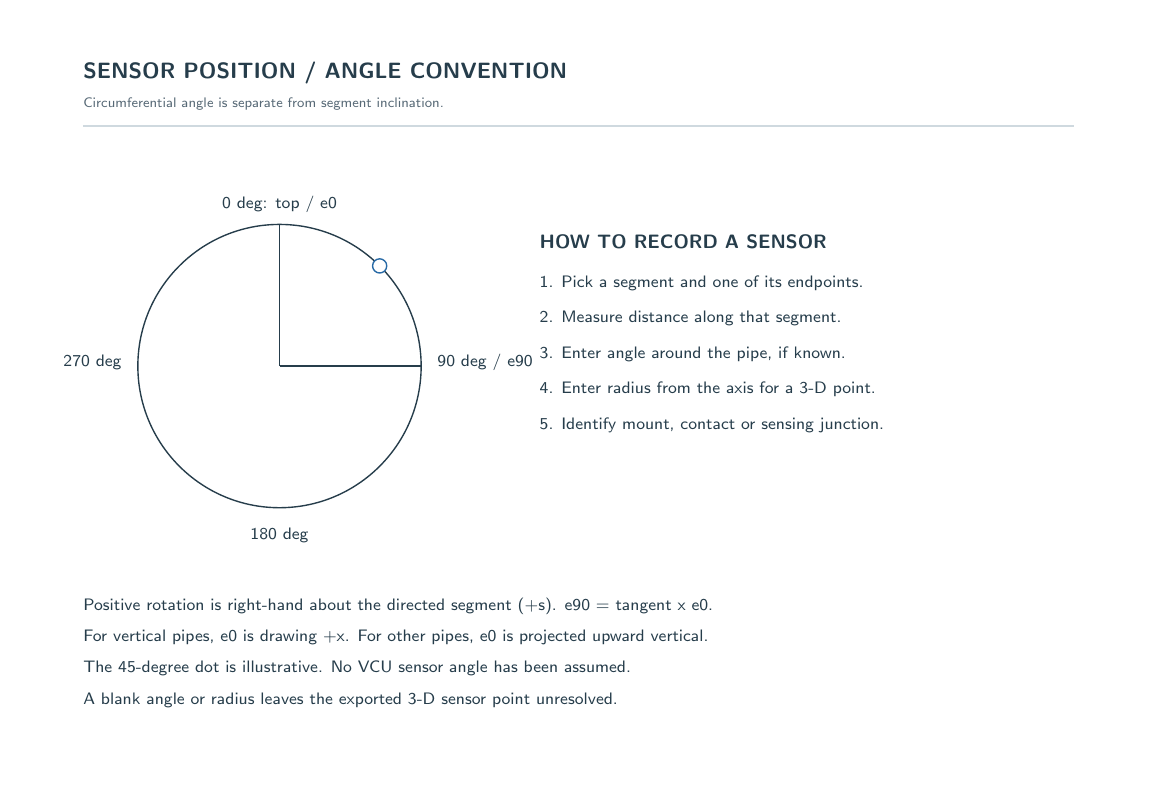
\begin{tikzpicture}[x=0.01cm,y=-0.01cm]
\path[use as bounding box] (0,0) rectangle (1400,950);
\definecolor{c263D4B}{HTML}{263D4B}
\definecolor{c286AA6}{HTML}{286AA6}
\definecolor{c576976}{HTML}{576976}
\definecolor{cCFD9DF}{HTML}{CFD9DF}
\node[anchor=base west,inner sep=0pt,text=c263D4B,font=\sffamily\fontsize{8.40}{10.20}\selectfont\bfseries] at (70.000,65.000) {SENSOR POSITION / ANGLE CONVENTION};
\node[anchor=base west,inner sep=0pt,text=c576976,font=\sffamily\fontsize{4.76}{5.78}\selectfont] at (70.000,102.000) {Circumferential angle is separate from segment inclination.};
\draw[draw=cCFD9DF,line width=0.520pt] (70.000,125.000) -- (1330.000,125.000);
\draw[fill=white,draw=c263D4B,line width=0.5pt] (320.000,430.000) circle (180);
\draw[draw=c263D4B,line width=0.520pt] (320.000,430.000) -- (320.000,250.000);
\draw[draw=c263D4B,line width=0.520pt] (320.000,430.000) -- (500.000,430.000);
\node[anchor=base,inner sep=0pt,text=c263D4B,font=\sffamily\fontsize{5.88}{7.14}\selectfont] at (320.000,230.000) {0 deg: top / e0};
\node[anchor=base west,inner sep=0pt,text=c263D4B,font=\sffamily\fontsize{5.88}{7.14}\selectfont] at (520.000,430.000) {90 deg / e90};
\node[anchor=base,inner sep=0pt,text=c263D4B,font=\sffamily\fontsize{5.88}{7.14}\selectfont] at (320.000,650.000) {180 deg};
\node[anchor=base east,inner sep=0pt,text=c263D4B,font=\sffamily\fontsize{5.88}{7.14}\selectfont] at (120.000,430.000) {270 deg};
\draw[fill=white,draw=c286AA6,line width=0.5pt] (447.279,302.721) circle (9);
\node[anchor=base west,inner sep=0pt,text=c263D4B,font=\sffamily\fontsize{6.72}{8.16}\selectfont\bfseries] at (650.000,280.000) {HOW TO RECORD A SENSOR};
\node[anchor=base west,inner sep=0pt,text=c263D4B,font=\sffamily\fontsize{5.60}{6.80}\selectfont] at (650.000,330.000) {1. Pick a segment and one of its endpoints.};
\node[anchor=base west,inner sep=0pt,text=c263D4B,font=\sffamily\fontsize{5.60}{6.80}\selectfont] at (650.000,375.000) {2. Measure distance along that segment.};
\node[anchor=base west,inner sep=0pt,text=c263D4B,font=\sffamily\fontsize{5.60}{6.80}\selectfont] at (650.000,420.000) {3. Enter angle around the pipe, if known.};
\node[anchor=base west,inner sep=0pt,text=c263D4B,font=\sffamily\fontsize{5.60}{6.80}\selectfont] at (650.000,465.000) {4. Enter radius from the axis for a 3-D point.};
\node[anchor=base west,inner sep=0pt,text=c263D4B,font=\sffamily\fontsize{5.60}{6.80}\selectfont] at (650.000,510.000) {5. Identify mount, contact or sensing junction.};
\node[anchor=base west,inner sep=0pt,text=c263D4B,font=\sffamily\fontsize{5.60}{6.80}\selectfont] at (70.000,740.000) {Positive rotation is right-hand about the directed segment (+s). e90 = tangent x e0.};
\node[anchor=base west,inner sep=0pt,text=c263D4B,font=\sffamily\fontsize{5.60}{6.80}\selectfont] at (70.000,780.000) {For vertical pipes, e0 is drawing +x. For other pipes, e0 is projected upward vertical.};
\node[anchor=base west,inner sep=0pt,text=c263D4B,font=\sffamily\fontsize{5.60}{6.80}\selectfont] at (70.000,820.000) {The 45-degree dot is illustrative. No VCU sensor angle has been assumed.};
\node[anchor=base west,inner sep=0pt,text=c263D4B,font=\sffamily\fontsize{5.60}{6.80}\selectfont] at (70.000,860.000) {A blank angle or radius leaves the exported 3-D sensor point unresolved.};
\end{tikzpicture}
}\end{center}
\clearpage\section{Current candidate input tables}\label{baseline-tables}
\subsection*{Main-loop geometry}
\small\setlength{\tabcolsep}{4pt}
\begin{longtable}{>{\raggedright\arraybackslash}p{0.23\textwidth}>{\raggedright\arraybackslash}p{0.12\textwidth}>{\raggedright\arraybackslash}p{0.16\textwidth}>{\raggedright\arraybackslash}p{0.14\textwidth}>{\raggedright\arraybackslash}p{0.22\textwidth}}
\toprule
\textbf{Segment} & \textbf{Endpoints} & \textbf{Length mm} & \textbf{Phi deg} & \textbf{Evidence} \\\midrule\endhead
upcomer & B to C & 1219.200 & 0.000 & CAD-derived \\[3pt]
upper\_left\_bend & C to D & \textit{Unknown} & \textit{Unknown} & CAD-derived \\[3pt]
cooler & D to E & 1352.550 & 100.800 & CAD-derived \\[3pt]
upper\_right\_bend & E to F & \textit{Unknown} & \textit{Unknown} & CAD-derived \\[3pt]
downcomer & F to G & 1228.669 & 180.000 & CAD-derived \\[3pt]
lower\_right\_bend & G to H & \textit{Unknown} & \textit{Unknown} & CAD-derived \\[3pt]
heater & H to A & 1346.496 & 280.794 & CAD-derived \\[3pt]
lower\_left\_bend & A to B & \textit{Unknown} & \textit{Unknown} & CAD-derived \\[3pt]
\bottomrule\end{longtable}\normalsize
Bends use offsets, not straight-length inputs. See the editable Geometry sheet and source length basis. The example forms do not populate these baseline cells.
\subsection*{Main-loop geometric sensor references}
\small\setlength{\tabcolsep}{4pt}
\begin{longtable}{>{\raggedright\arraybackslash}p{0.17\textwidth}>{\raggedright\arraybackslash}p{0.25\textwidth}>{\raggedright\arraybackslash}p{0.1\textwidth}>{\raggedright\arraybackslash}p{0.17\textwidth}>{\raggedright\arraybackslash}p{0.17\textwidth}}
\toprule
\textbf{Sensor} & \textbf{Segment} & \textbf{From} & \textbf{Distance mm} & \textbf{Angle deg} \\\midrule\endhead
STC-02 & upcomer & B & 116.686 & \textit{Unknown} \\[3pt]
STC-03 & upcomer & B & 446.886 & \textit{Unknown} \\[3pt]
STC-04 & upcomer & C & 492.914 & \textit{Unknown} \\[3pt]
STC-05 & upcomer & C & 277.014 & \textit{Unknown} \\[3pt]
LF-01 & upcomer & C & 61.114 & \textit{Unknown} \\[3pt]
STC-06 & cooler & D & 69.142 & \textit{Unknown} \\[3pt]
PTC-01 & cooler & D & 97.080 & \textit{Unknown} \\[3pt]
STC-07 & cooler & E & 155.331 & \textit{Unknown} \\[3pt]
LF-03 & cooler & E & 85.481 & \textit{Unknown} \\[3pt]
PTC-03 & cooler & E & 85.481 & \textit{Unknown} \\[3pt]
STC-08 & downcomer & F & 183.105 & \textit{Unknown} \\[3pt]
STC-09 & downcomer & F & 411.705 & \textit{Unknown} \\[3pt]
STC-10 & downcomer & G & 537.564 & \textit{Unknown} \\[3pt]
STC-11 & downcomer & G & 283.564 & \textit{Unknown} \\[3pt]
LF-04 & downcomer & G & 50.800 & \textit{Unknown} \\[3pt]
PTC-04 & heater & H & 63.716 & \textit{Unknown} \\[3pt]
STC-12 & heater & H & 69.293 & \textit{Unknown} \\[3pt]
LF-02 & heater & A & 83.394 & \textit{Unknown} \\[3pt]
PTC-02 & heater & A & 83.394 & \textit{Unknown} \\[3pt]
STC-01 & heater & A & 49.428 & \textit{Unknown} \\[3pt]
\bottomrule\end{longtable}\normalsize
JTC-A/B are retained in Calibration, but jacket-port positions are not yet drawn. DAQ mappings, calibration and model mappings remain unknown unless separately entered with evidence.
\subsection*{VCU fluid choices}
Prop-30, air and water are permitted candidate options from the user. A circuit/run assignment is still required. The supplied draft phase campaign is Prop-30-specific.
\small\setlength{\tabcolsep}{4pt}
\begin{longtable}{>{\raggedright\arraybackslash}p{0.15\textwidth}>{\raggedright\arraybackslash}p{0.3\textwidth}>{\raggedright\arraybackslash}p{0.22\textwidth}>{\raggedright\arraybackslash}p{0.2\textwidth}}
\toprule
\textbf{Fluid} & \textbf{Product} & \textbf{Circuit} & \textbf{Range C} \\\midrule\endhead
PROP30 & Propylene glycol / water & Primary-loop candidate; select per run & \textit{Unknown} \\[3pt]
AIR & Air & Primary-loop option and room ambient; distinguish per run & \textit{Unknown} \\[3pt]
WATER & Water & Reported jacket coolant; primary-loop option per run & \textit{Unknown} \\[3pt]
\bottomrule\end{longtable}\normalsize
\clearpage\section{Insulation region records}\label{insulation-detail}
The Insulation regions workbook tab is the regional coverage record. Each state applies to the whole named region. Unknown coverage is distinct from confirmed bare pipe. Material and thickness are optional recorded inputs; no thermal resistance is calculated.
For the cooler, identify whether insulation covers the jacket exterior or another surface in Notes. Jacket-based partitions describe mechanical extents and do not establish active cooling boundaries. The older Geometry insulation field is retained for compatibility; it does not populate or override this register.
\par\noindent\begin{minipage}{\textwidth}\small\setlength{\parskip}{2pt}
{\bfseries INS-01 | Upcomer}\par
\textbf{Coverage:} Insulated\par
\textbf{Segment / boundary reference:} upcomer / Full segment\par
\textbf{Boundary basis / source:} CAD-derived / VCU-R9-E01 (2026-10-08) sheets 1-3\par
\textbf{Stations:} 0.000 to 1219.200 mm from segment Start\par
\textbf{Insulated surface / notes:} Reported ordinary main-pipe fiberglass assignment, approximately 2 in; regional model candidate, not installed product/thickness validation. Local STC contacts/transition details remain separate.\par
\textbf{Material ID / thickness mm:} MAIN-INS / 50.8\par
\textbf{Evidence type:} Reported\par
\textbf{Evidence file / location:} support/evidence/2026-10-16\_\allowbreak{}GEO-010\_\allowbreak{}regional\_\allowbreak{}insulation\_\allowbreak{}sync/insulation.yaml / regions; VREG; VCU-007/008 and GEO-009\par
\end{minipage}\par\vspace{5pt}
\par\noindent\begin{minipage}{\textwidth}\small\setlength{\parskip}{2pt}
{\bfseries INS-02 | Top-left corner}\par
\textbf{Coverage:} Insulated\par
\textbf{Segment / boundary reference:} upper\_\allowbreak{}left\_\allowbreak{}bend / Full schematic corner\par
\textbf{Boundary basis / source:} CAD-derived / VCU-R9-E01 (2026-10-08) sheets 1-3\par
\textbf{Stations:} No qualified station interval; see geometry qualification\par
\textbf{Insulated surface / notes:} Reported ordinary main-pipe fiberglass assignment, approximately 2 in; regional model candidate, not installed product/thickness validation. Local STC contacts/transition details remain separate.\par
\textbf{Material ID / thickness mm:} MAIN-INS / 50.8\par
\textbf{Evidence type:} Reported\par
\textbf{Evidence file / location:} support/evidence/2026-10-16\_\allowbreak{}GEO-010\_\allowbreak{}regional\_\allowbreak{}insulation\_\allowbreak{}sync/insulation.yaml / regions; VREG; VCU-007/008 and GEO-009\par
\end{minipage}\par\vspace{5pt}
\par\noindent\begin{minipage}{\textwidth}\small\setlength{\parskip}{2pt}
{\bfseries INS-03 | Pre-cooler}\par
\textbf{Coverage:} Bare\par
\textbf{Segment / boundary reference:} cooler / Segment start to Complete jacket start\par
\textbf{Boundary basis / source:} CAD-derived; mechanical jacket envelope; provisional insulation partition / VCU-R9-E01 (2026-10-08) sheet 3\par
\textbf{Stations:} 0.000 to 127.562 mm from segment Start\par
\textbf{Insulated surface / notes:} Reported straight top D-E bare, GEO-008 retained; water jacket remains present.\par
\textbf{Material ID / thickness mm:} Unknown / Unknown\par
\textbf{Evidence type:} Reported\par
\textbf{Evidence file / location:} support/evidence/2026-10-16\_\allowbreak{}GEO-010\_\allowbreak{}regional\_\allowbreak{}insulation\_\allowbreak{}sync/insulation.yaml / regions; VREG; VCU-007/008 and GEO-009\par
\end{minipage}\par\vspace{5pt}
\par\noindent\begin{minipage}{\textwidth}\small\setlength{\parskip}{2pt}
{\bfseries INS-04 | Cooler}\par
\textbf{Coverage:} Bare\par
\textbf{Segment / boundary reference:} cooler / Complete jacket start to Complete jacket end\par
\textbf{Boundary basis / source:} CAD-derived; mechanical jacket envelope; provisional insulation partition / VCU-R9-E01 (2026-10-08) sheet 3\par
\textbf{Stations:} 127.562 to 1157.849 mm from segment Start\par
\textbf{Insulated surface / notes:} Reported straight top D-E bare, GEO-008 retained; water jacket remains present.\par
\textbf{Material ID / thickness mm:} Unknown / Unknown\par
\textbf{Evidence type:} Reported\par
\textbf{Evidence file / location:} support/evidence/2026-10-16\_\allowbreak{}GEO-010\_\allowbreak{}regional\_\allowbreak{}insulation\_\allowbreak{}sync/insulation.yaml / regions; VREG; VCU-007/008 and GEO-009\par
\end{minipage}\par\vspace{5pt}
\clearpage{\large\bfseries Insulation region records --- continued}\par
\par\noindent\begin{minipage}{\textwidth}\small\setlength{\parskip}{2pt}
{\bfseries INS-05 | Post-cooler}\par
\textbf{Coverage:} Bare\par
\textbf{Segment / boundary reference:} cooler / Complete jacket end to segment end\par
\textbf{Boundary basis / source:} CAD-derived; mechanical jacket envelope; provisional insulation partition / VCU-R9-E01 (2026-10-08) sheet 3\par
\textbf{Stations:} 1157.849 to 1352.550 mm from segment Start\par
\textbf{Insulated surface / notes:} Reported straight top D-E bare, GEO-008 retained; water jacket remains present.\par
\textbf{Material ID / thickness mm:} Unknown / Unknown\par
\textbf{Evidence type:} Reported\par
\textbf{Evidence file / location:} support/evidence/2026-10-16\_\allowbreak{}GEO-010\_\allowbreak{}regional\_\allowbreak{}insulation\_\allowbreak{}sync/insulation.yaml / regions; VREG; VCU-007/008 and GEO-009\par
\end{minipage}\par\vspace{5pt}
\par\noindent\begin{minipage}{\textwidth}\small\setlength{\parskip}{2pt}
{\bfseries INS-06 | Top-right corner}\par
\textbf{Coverage:} Insulated\par
\textbf{Segment / boundary reference:} upper\_\allowbreak{}right\_\allowbreak{}bend / Full schematic corner\par
\textbf{Boundary basis / source:} CAD-derived / VCU-R9-E01 (2026-10-08) sheets 1-3\par
\textbf{Stations:} No qualified station interval; see geometry qualification\par
\textbf{Insulated surface / notes:} Reported ordinary main-pipe fiberglass assignment, approximately 2 in; regional model candidate, not installed product/thickness validation. Local STC contacts/transition details remain separate.\par
\textbf{Material ID / thickness mm:} MAIN-INS / 50.8\par
\textbf{Evidence type:} Reported\par
\textbf{Evidence file / location:} support/evidence/2026-10-16\_\allowbreak{}GEO-010\_\allowbreak{}regional\_\allowbreak{}insulation\_\allowbreak{}sync/insulation.yaml / regions; VREG; VCU-007/008 and GEO-009\par
\end{minipage}\par\vspace{5pt}
\par\noindent\begin{minipage}{\textwidth}\small\setlength{\parskip}{2pt}
{\bfseries INS-07 | Downcomer}\par
\textbf{Coverage:} Insulated\par
\textbf{Segment / boundary reference:} downcomer / Full segment\par
\textbf{Boundary basis / source:} CAD-derived / VCU-R9-E01 (2026-10-08) sheets 1-3\par
\textbf{Stations:} 0.000 to 1228.669 mm from segment Start\par
\textbf{Insulated surface / notes:} Reported ordinary main-pipe fiberglass assignment, approximately 2 in; regional model candidate, not installed product/thickness validation. Local STC contacts/transition details remain separate.\par
\textbf{Material ID / thickness mm:} MAIN-INS / 50.8\par
\textbf{Evidence type:} Reported\par
\textbf{Evidence file / location:} support/evidence/2026-10-16\_\allowbreak{}GEO-010\_\allowbreak{}regional\_\allowbreak{}insulation\_\allowbreak{}sync/insulation.yaml / regions; VREG; VCU-007/008 and GEO-009\par
\end{minipage}\par\vspace{5pt}
\clearpage{\large\bfseries Insulation region records --- continued}\par
\par\noindent\begin{minipage}{\textwidth}\small\setlength{\parskip}{2pt}
{\bfseries INS-08 | Bottom-right corner}\par
\textbf{Coverage:} Insulated\par
\textbf{Segment / boundary reference:} lower\_\allowbreak{}right\_\allowbreak{}bend / Full schematic corner\par
\textbf{Boundary basis / source:} CAD-derived / VCU-R9-E01 (2026-10-08) sheets 1-3\par
\textbf{Stations:} No qualified station interval; see geometry qualification\par
\textbf{Insulated surface / notes:} Reported ordinary main-pipe fiberglass assignment, approximately 2 in; regional model candidate, not installed product/thickness validation. Local STC contacts/transition details remain separate.\par
\textbf{Material ID / thickness mm:} MAIN-INS / 50.8\par
\textbf{Evidence type:} Reported\par
\textbf{Evidence file / location:} support/evidence/2026-10-16\_\allowbreak{}GEO-010\_\allowbreak{}regional\_\allowbreak{}insulation\_\allowbreak{}sync/insulation.yaml / regions; VREG; VCU-007/008 and GEO-009\par
\end{minipage}\par\vspace{5pt}
\par\noindent\begin{minipage}{\textwidth}\small\setlength{\parskip}{2pt}
{\bfseries INS-09 | Heater}\par
\textbf{Coverage:} Insulated\par
\textbf{Segment / boundary reference:} heater / Full segment\par
\textbf{Boundary basis / source:} CAD-derived / VCU-R9-E01 (2026-10-08) sheets 1-3\par
\textbf{Stations:} 0.000 to 1346.496 mm from segment Start\par
\textbf{Insulated surface / notes:} Reported heater insulation: approximately 1/4 in calcium-aluminum-silicate ceramic-fiber strip only; no extra fiberglass. Thickness is an estimate, not measured.\par
\textbf{Material ID / thickness mm:} HEATER-INS / 6.35\par
\textbf{Evidence type:} Reported\par
\textbf{Evidence file / location:} support/evidence/2026-10-16\_\allowbreak{}GEO-010\_\allowbreak{}regional\_\allowbreak{}insulation\_\allowbreak{}sync/insulation.yaml / regions; VREG; VCU-007/008 and GEO-009\par
\end{minipage}\par\vspace{5pt}
\par\noindent\begin{minipage}{\textwidth}\small\setlength{\parskip}{2pt}
{\bfseries INS-10 | Bottom-left corner}\par
\textbf{Coverage:} Insulated\par
\textbf{Segment / boundary reference:} lower\_\allowbreak{}left\_\allowbreak{}bend / Full schematic corner\par
\textbf{Boundary basis / source:} CAD-derived / VCU-R9-E01 (2026-10-08) sheets 1-3\par
\textbf{Stations:} No qualified station interval; see geometry qualification\par
\textbf{Insulated surface / notes:} Reported ordinary main-pipe fiberglass assignment, approximately 2 in; regional model candidate, not installed product/thickness validation. Local STC contacts/transition details remain separate.\par
\textbf{Material ID / thickness mm:} MAIN-INS / 50.8\par
\textbf{Evidence type:} Reported\par
\textbf{Evidence file / location:} support/evidence/2026-10-16\_\allowbreak{}GEO-010\_\allowbreak{}regional\_\allowbreak{}insulation\_\allowbreak{}sync/insulation.yaml / regions; VREG; VCU-007/008 and GEO-009\par
\end{minipage}\par\vspace{5pt}
\clearpage\section{Complete requirements and evidence register}\label{requirements}
The Requirements workbook tab is the editable master. Each record states why the field is needed, who should supply it, where the requirement and evidence came from, what uses it supports, and what remains unresolved. Requirement provenance is distinct from evidence for a value.
\textbf{Review rule:} the records below describe candidate evidence. Approved choices require a recorded decision, scope and effective configuration; none has been established in this seed package.
\par\noindent\begin{minipage}{\textwidth}\small\setlength{\parskip}{2pt}
\subsection*{C01 | Facility and configuration ID}
\textbf{Purpose:} Tie measurements to one physical setup.\par
\textbf{Package / responsible team:} Configuration / Experimental team\par
\textbf{Applies to:} VCU; every configuration and affected run\par
\textbf{Requirement source / locator:} P0; Section 3 Method, document facility configuration\par
\textbf{Current evidence [Reported]:} VCU; prototype ID VCU-REV9-DRAFT-001\par
\textbf{Evidence source / locator:} USER / current workbook; Facility selection; Start sheet\par
\textbf{Review state:} Needs review\par
\textbf{Selected choice:} None selected\par
\textbf{Decision scope / rationale:} \textit{Unknown}\par
\textbf{Reviewer / date; effective configuration:} Pending; Unknown\par
\textbf{To resolve:} Which installed configuration and effective date does this identify?\par
\end{minipage}\par\vspace{5pt}
\par\noindent\begin{minipage}{\textwidth}\small\setlength{\parskip}{2pt}
\subsection*{C02 | Effective date and change history}
\textbf{Purpose:} Explain what changed between datasets.\par
\textbf{Package / responsible team:} Configuration / Experimental team\par
\textbf{Applies to:} VCU; every configuration and affected run\par
\textbf{Requirement source / locator:} P0; DESIGN; Campaign execution conventions; proposed revision log\par
\textbf{Current evidence [Reported]:} 2026-10-16 / VCU-REV9-DRAFT-002: PTC-X removed from active sensor and calibration records at the repository owner's request. Documentation change only; no physical removal or installed-hardware verification is asserted. 2026-10-16 / VCU-REV9-DRAFT-003: added ten insulation coverage regions and the diagram; all coverage Unknown pending evidence.\par
\textbf{Evidence source / locator:} USER; Start effective date and change summary; previous record saved at support/checkpoints/2026-10-16\_\allowbreak{}VCU-REV9-DRAFT-002/. Owner-approved insulation feature plan in the Codex session, 2026-10-16; installed coverage remains unconfirmed.\par
\textbf{Review state:} Needs review\par
\textbf{Selected choice:} None selected\par
\textbf{Decision scope / rationale:} \textit{Unknown}\par
\textbf{Reviewer / date; effective configuration:} Pending; Unknown\par
\textbf{To resolve:} Record effective date, author, changed item, reason, previous/new evidence, affected runs and whether recalibration or model revalidation is needed.\par
\end{minipage}\par\vspace{5pt}
\par\noindent\begin{minipage}{\textwidth}\small\setlength{\parskip}{2pt}
\subsection*{C03 | Reviewer, date and approved use}
\textbf{Purpose:} Record an actual release decision separately from evidence type.\par
\textbf{Package / responsible team:} Shared / Facility lead / package reviewer\par
\textbf{Applies to:} VCU; every configuration and affected run\par
\textbf{Requirement source / locator:} P0; Approval record and Section 3 Disposition\par
\textbf{Current evidence [Unknown]:} Unknown\par
\textbf{Evidence source / locator:} None supplied; Not available\par
\textbf{Review state:} Needs information\par
\textbf{Selected choice:} None selected\par
\textbf{Decision scope / rationale:} \textit{Unknown}\par
\textbf{Reviewer / date; effective configuration:} Pending; Unknown\par
\textbf{To resolve:} Who may release the package, and for which experiment/model use?\par
\end{minipage}\par\vspace{5pt}
\par\noindent\begin{minipage}{\textwidth}\small\setlength{\parskip}{2pt}
\subsection*{C04 | Source revision and file hash}
\textbf{Purpose:} Make the geometry baseline reproducible.\par
\textbf{Package / responsible team:} Shared / Experimental + computational\par
\textbf{Applies to:} VCU; 1-D and CFD / CHT\par
\textbf{Requirement source / locator:} R9; Sheet 8 source identity\par
\textbf{Current evidence [Reported]:} Rev9 is user-selected best current geometry for new work; existing solver/results remain versioned Rev8.\par
\textbf{Evidence source / locator:} VSEL; WORK; See cited Sources locators and Current knowledge / Native channels; CFG-002 evidence bundle\par
\textbf{Review state:} Needs review\par
\textbf{Selected choice:} Rev9 for new configuration documentation; no historical run migration\par
\textbf{Decision scope / rationale:} Transferred documented working understanding; provisional use only; no installed or package release approval.\par
\textbf{Reviewer / date; effective configuration:} Pending; VCU-REV9-DRAFT-007\par
\textbf{To resolve:} Confirm installed configuration and dates; no physical release implied.\par
\end{minipage}\par\vspace{5pt}
\par\noindent\begin{minipage}{\textwidth}\small\setlength{\parskip}{2pt}
\subsection*{C05 | Coordinate datum and axes}
\textbf{Purpose:} Give every location the same reference.\par
\textbf{Package / responsible team:} Configuration / Experimental + computational\par
\textbf{Applies to:} VCU; 1-D and CFD / CHT\par
\textbf{Requirement source / locator:} R9; Sheets 1 and 7\par
\textbf{Current evidence [CAD-derived]:} B origin; x right; y up; n normal; B-C-D-E-F-G-H-A-B\par
\textbf{Evidence source / locator:} R9; Sheets 1, 7\par
\textbf{Review state:} Needs review\par
\textbf{Selected choice:} None selected\par
\textbf{Decision scope / rationale:} \textit{Unknown}\par
\textbf{Reviewer / date; effective configuration:} Pending; Unknown\par
\textbf{To resolve:} Identify these points on a dated hardware photo.\par
\end{minipage}\par\vspace{5pt}
\par\noindent\begin{minipage}{\textwidth}\small\setlength{\parskip}{2pt}
\subsection*{C06 | Segment endpoints and straight length}
\textbf{Purpose:} Define the length being measured.\par
\textbf{Package / responsible team:} Configuration / Experimental team\par
\textbf{Applies to:} VCU; 1-D and CFD / CHT\par
\textbf{Requirement source / locator:} P0; SEG; Method geometry map; segment rows\par
\textbf{Current evidence [CAD-derived]:} Upcomer B-C 1219.200 mm; other spans in SEG\par
\textbf{Evidence source / locator:} SEG; upcomer row: reference\_\allowbreak{}length\_\allowbreak{}mm and length\_\allowbreak{}basis\par
\textbf{Review state:} Needs review\par
\textbf{Selected choice:} None selected\par
\textbf{Decision scope / rationale:} \textit{Unknown}\par
\textbf{Reviewer / date; effective configuration:} Pending; Unknown\par
\textbf{To resolve:} Measure axis-end span; do not substitute virtual-corner length.\par
\end{minipage}\par\vspace{5pt}
\par\noindent\begin{minipage}{\textwidth}\small\setlength{\parskip}{2pt}
\subsection*{C07 | Installed inclination and gravity direction}
\textbf{Purpose:} Determine elevation changes and buoyancy orientation.\par
\textbf{Package / responsible team:} Configuration / Experimental team\par
\textbf{Applies to:} VCU; 1-D and CFD / CHT\par
\textbf{Requirement source / locator:} P0; R9; Method geometry map; sheets 1-2\par
\textbf{Current evidence [Modeling assumption]:} Geometry-derived inclined axes about 10.8 deg; working local gravity (0,-1,0). Installed gravity survey absent.\par
\textbf{Evidence source / locator:} VSEL; WORK; See cited Sources locators and Current knowledge / Native channels; CFG-002 evidence bundle\par
\textbf{Review state:} Needs review\par
\textbf{Selected choice:} Use current local drawing frame and geometry-derived inclination provisionally\par
\textbf{Decision scope / rationale:} Transferred documented working understanding; provisional use only; no installed or package release approval.\par
\textbf{Reviewer / date; effective configuration:} Pending; VCU-REV9-DRAFT-007\par
\textbf{To resolve:} Installed tilt/gravity and uncertainty still need survey.\par
\end{minipage}\par\vspace{5pt}
\par\noindent\begin{minipage}{\textwidth}\small\setlength{\parskip}{2pt}
\subsection*{C08 | Bend geometry and length basis}
\textbf{Purpose:} Avoid replacing a chord with an arc.\par
\textbf{Package / responsible team:} Configuration / Experimental + computational\par
\textbf{Applies to:} VCU; 1-D and CFD / CHT\par
\textbf{Requirement source / locator:} SEG; Bend rows and length\_\allowbreak{}basis\par
\textbf{Current evidence [CAD-derived]:} Three torus arcs; G-H recovered spine qualified; exact joined path unresolved\par
\textbf{Evidence source / locator:} SEG; R9; Bend rows; sheet 2\par
\textbf{Review state:} Needs review\par
\textbf{Selected choice:} None selected\par
\textbf{Decision scope / rationale:} \textit{Unknown}\par
\textbf{Reviewer / date; effective configuration:} Pending; Unknown\par
\textbf{To resolve:} How will the physical bend be measured and represented?\par
\end{minipage}\par\vspace{5pt}
\par\noindent\begin{minipage}{\textwidth}\small\setlength{\parskip}{2pt}
\subsection*{C09 | Pipe inside diameter}
\textbf{Purpose:} Set fluid area, inventory and hydraulic dimension.\par
\textbf{Package / responsible team:} Configuration / Experimental team\par
\textbf{Applies to:} VCU; 1-D and CFD / CHT\par
\textbf{Requirement source / locator:} P0; DIA; Geometry map; Main swept loop\par
\textbf{Current evidence [Reported]:} CAD main bore absent. GEO-008 retains 26.64 mm rounded nominal ID for provisional main piping; not a CAD-extracted bore or installed measurement. Local spool bores differ.\par
\textbf{Evidence source / locator:} DIA; VSEL; Main swept loop; GEO-008 main nominal ID; CAD dimensions tab\par
\textbf{Review state:} Needs review\par
\textbf{Selected choice:} None selected\par
\textbf{Decision scope / rationale:} \textit{Unknown}\par
\textbf{Reviewer / date; effective configuration:} Pending; Unknown\par
\textbf{To resolve:} Confirm actual bore/specification and local restrictions; keep CAD null.\par
\end{minipage}\par\vspace{5pt}
\par\noindent\begin{minipage}{\textwidth}\small\setlength{\parskip}{2pt}
\subsection*{C10 | Pipe outside diameter}
\textbf{Purpose:} Set wall and external thermal geometry.\par
\textbf{Package / responsible team:} Configuration / Experimental team\par
\textbf{Applies to:} VCU; 1-D and CFD / CHT\par
\textbf{Requirement source / locator:} DIA; Main swept loop row\par
\textbf{Current evidence [CAD-derived]:} 33.401 mm CAD OD\par
\textbf{Evidence source / locator:} DIA; Main swept loop / outer\_\allowbreak{}diameter\_\allowbreak{}mm\par
\textbf{Review state:} Needs review\par
\textbf{Selected choice:} None selected\par
\textbf{Decision scope / rationale:} \textit{Unknown}\par
\textbf{Reviewer / date; effective configuration:} Pending; Unknown\par
\textbf{To resolve:} Confirm installed OD and measurement uncertainty.\par
\end{minipage}\par\vspace{5pt}
\par\noindent\begin{minipage}{\textwidth}\small\setlength{\parskip}{2pt}
\subsection*{C11 | Pipe material grade and certificate}
\textbf{Purpose:} Identify the solid whose properties will be used.\par
\textbf{Package / responsible team:} Configuration / Experimental team\par
\textbf{Applies to:} VCU; 1-D and CFD / CHT\par
\textbf{Requirement source / locator:} P0; MAT; Geometry map; VCU Piping\par
\textbf{Current evidence [Reported]:} 316L, nominal 1-inch schedule 40 reported\par
\textbf{Evidence source / locator:} MAT; VCU Piping lines 23-27\par
\textbf{Review state:} Needs review\par
\textbf{Selected choice:} None selected\par
\textbf{Decision scope / rationale:} \textit{Unknown}\par
\textbf{Reviewer / date; effective configuration:} Pending; Unknown\par
\textbf{To resolve:} Provide purchase/specification or material certificate.\par
\end{minipage}\par\vspace{5pt}
\par\noindent\begin{minipage}{\textwidth}\small\setlength{\parskip}{2pt}
\subsection*{C12 | Dimension uncertainty and method}
\textbf{Purpose:} Propagate measurement uncertainty without using CAD print precision.\par
\textbf{Package / responsible team:} Configuration / Experimental team\par
\textbf{Applies to:} VCU; 1-D and CFD / CHT\par
\textbf{Requirement source / locator:} P0; DESIGN; Measurement uncertainties; proposed geometry uncertainty field\par
\textbf{Current evidence [Unknown]:} Unknown\par
\textbf{Evidence source / locator:} None supplied; Not available\par
\textbf{Review state:} Needs information\par
\textbf{Selected choice:} None selected\par
\textbf{Decision scope / rationale:} \textit{Unknown}\par
\textbf{Reviewer / date; effective configuration:} Pending; Unknown\par
\textbf{To resolve:} Record method, instrument, repeatability and uncertainty units for each dimension.\par
\end{minipage}\par\vspace{5pt}
\par\noindent\begin{minipage}{\textwidth}\small\setlength{\parskip}{2pt}
\subsection*{C13 | Insulation product and layer order}
\textbf{Purpose:} Identify the actual thermal stack.\par
\textbf{Package / responsible team:} Configuration / Experimental team\par
\textbf{Applies to:} VCU; 1-D and CFD / CHT\par
\textbf{Requirement source / locator:} P0; MAT; Geometry map; VCU insulation\par
\textbf{Current evidence [Reported]:} Ordinary main piping (upcomer/downcomer and four corners): fiberglass MAIN-INS; heater: calcium-aluminum-silicate HEATER-INS strip only, no additional fiberglass.\par
\textbf{Evidence source / locator:} VREG; VTOP; VREG regional YAML and ADR-0025/0026; VTOP corner/LF-01 correction; user reaffirmation 2026-10-16\par
\textbf{Review state:} Needs review\par
\textbf{Selected choice:} None selected\par
\textbf{Decision scope / rationale:} \textit{Unknown}\par
\textbf{Reviewer / date; effective configuration:} Pending; Unknown\par
\textbf{To resolve:} Which product and layers are installed on this exact segment?\par
\end{minipage}\par\vspace{5pt}
\par\noindent\begin{minipage}{\textwidth}\small\setlength{\parskip}{2pt}
\subsection*{C14 | Insulation thickness by section}
\textbf{Purpose:} Set the thermal resistance geometry.\par
\textbf{Package / responsible team:} Configuration / Experimental team\par
\textbf{Applies to:} VCU; 1-D and CFD / CHT\par
\textbf{Requirement source / locator:} P0; MAT; Geometry map; VCU insulation\par
\textbf{Current evidence [Reported]:} Reported estimates: ordinary insulated regions 50.8 mm (2 in); heater strip 6.35 mm (1/4 in). Not installed thickness measurements.\par
\textbf{Evidence source / locator:} VREG; VTOP; VREG regional YAML and ADR-0025/0026; VTOP corner/LF-01 correction; user reaffirmation 2026-10-16\par
\textbf{Review state:} Needs review\par
\textbf{Selected choice:} None selected\par
\textbf{Decision scope / rationale:} \textit{Unknown}\par
\textbf{Reviewer / date; effective configuration:} Pending; Unknown\par
\textbf{To resolve:} Measure each layer; do not apply either value everywhere.\par
\end{minipage}\par\vspace{5pt}
\par\noindent\begin{minipage}{\textwidth}\small\setlength{\parskip}{2pt}
\subsection*{C15 | Coverage start/end, gaps and condition}
\textbf{Purpose:} Capture uninsulated heat-loss paths.\par
\textbf{Package / responsible team:} Configuration / Experimental team\par
\textbf{Applies to:} VCU; 1-D and CFD / CHT\par
\textbf{Requirement source / locator:} P0; Method: facility and fluid configuration; geometry map\par
\textbf{Current evidence [Reported]:} Reported coverage known for all ten regions: upcomer/downcomer, four corners and heater insulated; pre-cooler/jacket/post-cooler D-E bare. LF-01 covered. Exact local contacts and transitions remain open.\par
\textbf{Evidence source / locator:} VREG; VTOP; VREG regional YAML and ADR-0025/0026; VTOP corner/LF-01 correction; user reaffirmation 2026-10-16\par
\textbf{Review state:} Needs review\par
\textbf{Selected choice:} None selected\par
\textbf{Decision scope / rationale:} \textit{Unknown}\par
\textbf{Reviewer / date; effective configuration:} Pending; Unknown\par
\textbf{To resolve:} Supply evidence and request review.\par
\end{minipage}\par\vspace{5pt}
\par\noindent\begin{minipage}{\textwidth}\small\setlength{\parskip}{2pt}
\subsection*{C16 | Insulation contact and support details}
\textbf{Purpose:} Represent contact resistance and support heat paths.\par
\textbf{Package / responsible team:} Shared / Experimental + computational\par
\textbf{Applies to:} VCU; 1-D and CFD / CHT\par
\textbf{Requirement source / locator:} P0; HEAT; Geometry map; VCU Insulation\par
\textbf{Current evidence [Modeling assumption]:} Perfect thermal contact is a user-directed model assumption (VINS), not a surveyed contact condition. Actual supports, gaps and layers remain open.\par
\textbf{Evidence source / locator:} VINS; insulation.yaml contact\par
\textbf{Review state:} Needs review\par
\textbf{Selected choice:} None selected\par
\textbf{Decision scope / rationale:} \textit{Unknown}\par
\textbf{Reviewer / date; effective configuration:} Pending; Unknown\par
\textbf{To resolve:} Is there evidence of contact, compression, gaps or support conduction?\par
\end{minipage}\par\vspace{5pt}
\par\noindent\begin{minipage}{\textwidth}\small\setlength{\parskip}{2pt}
\subsection*{C17 | Dated overview and detail photos}
\textbf{Purpose:} Make the configuration recognizable and auditable.\par
\textbf{Package / responsible team:} Configuration / Experimental team\par
\textbf{Applies to:} VCU; every configuration and affected run\par
\textbf{Requirement source / locator:} USER; DESIGN; Requested form-like geometry package\par
\textbf{Current evidence [Reported]:} Supplied images are illustrations; not a dated installed survey\par
\textbf{Evidence source / locator:} USER; Supplied VCU image captions\par
\textbf{Review state:} Needs review\par
\textbf{Selected choice:} None selected\par
\textbf{Decision scope / rationale:} \textit{Unknown}\par
\textbf{Reviewer / date; effective configuration:} Pending; Unknown\par
\textbf{To resolve:} Attach photos showing endpoints, insulation and sensors with scale.\par
\end{minipage}\par\vspace{5pt}
\par\noindent\begin{minipage}{\textwidth}\small\setlength{\parskip}{2pt}
\subsection*{C18 | Fluid identity and circuit assignment}
\textbf{Purpose:} Avoid confusing working fluid, coolant and room air.\par
\textbf{Package / responsible team:} Configuration / Experimental team\par
\textbf{Applies to:} VCU; every configuration and affected run\par
\textbf{Requirement source / locator:} USER; P0; Fluid scope; facility/fluid configuration\par
\textbf{Current evidence [Reported]:} VCU options Prop-30/air/water; primary fill selected per run. Jacket water reported; ambient air role distinct.\par
\textbf{Evidence source / locator:} USER; FLUIDCFG; XWALK; WORK; See cited Sources locators and Current knowledge / Native channels; CFG-002 evidence bundle\par
\textbf{Review state:} Needs review\par
\textbf{Selected choice:} Run-specific primary fill; reported water jacket coolant\par
\textbf{Decision scope / rationale:} Transferred documented working understanding; provisional use only; no installed or package release approval.\par
\textbf{Reviewer / date; effective configuration:} Pending; VCU-REV9-DRAFT-007\par
\textbf{To resolve:} Confirm fluid/batch in each acquisition; ambient filename alone is insufficient.\par
\end{minipage}\par\vspace{5pt}
\par\noindent\begin{minipage}{\textwidth}\small\setlength{\parskip}{2pt}
\subsection*{C19 | Composition and concentration basis}
\textbf{Purpose:} Select the correct property family.\par
\textbf{Package / responsible team:} Configuration / Experimental team\par
\textbf{Applies to:} VCU mixtures\par
\textbf{Requirement source / locator:} P0; Method fluid configuration\par
\textbf{Current evidence [Reported]:} Prop-30: 30\% propylene glycol by mass reported\par
\textbf{Evidence source / locator:} MAT; PG; MAT lines 19-21; PG 30 wt\% note\par
\textbf{Review state:} Needs review\par
\textbf{Selected choice:} None selected\par
\textbf{Decision scope / rationale:} \textit{Unknown}\par
\textbf{Reviewer / date; effective configuration:} Pending; Unknown\par
\textbf{To resolve:} Identify formulation, preparation and concentration verification.\par
\end{minipage}\par\vspace{5pt}
\par\noindent\begin{minipage}{\textwidth}\small\setlength{\parskip}{2pt}
\subsection*{C20 | Batch, fill inventory and condition}
\textbf{Purpose:} Reproduce thermal capacity and hydraulic state.\par
\textbf{Package / responsible team:} Configuration / Experimental team\par
\textbf{Applies to:} VCU; every configuration and affected run\par
\textbf{Requirement source / locator:} P0; P2; P0 fluid configuration; P2 fill record\par
\textbf{Current evidence [Unknown]:} Unknown\par
\textbf{Evidence source / locator:} None supplied; Not available\par
\textbf{Review state:} Needs information\par
\textbf{Selected choice:} None selected\par
\textbf{Decision scope / rationale:} \textit{Unknown}\par
\textbf{Reviewer / date; effective configuration:} Pending; Unknown\par
\textbf{To resolve:} Record batch, fill date, mass/level, contamination and trapped-gas evidence.\par
\end{minipage}\par\vspace{5pt}
\par\noindent\begin{minipage}{\textwidth}\small\setlength{\parskip}{2pt}
\subsection*{C21 | Sensor hardware ID and type}
\textbf{Purpose:} Identify the installed instrument independently of a CAD label.\par
\textbf{Package / responsible team:} Configuration / Experimental team\par
\textbf{Applies to:} VCU; every configuration and affected run\par
\textbf{Requirement source / locator:} P0; SNS; Instrumentation documentation; sensor rows\par
\textbf{Current evidence [Reported]:} Active geometry: 12 STC, 4 main PTC, 4 LF and 2 JTC = 22 references; 20 main-loop references. Original extraction has 23 including excluded PTC-X. Native core inventory has 20 channels incl. Amb/Tank; LF is not mapped.\par
\textbf{Evidence source / locator:} VSEL; WORK; XWALK; See cited Sources locators and Current knowledge / Native channels; CFG-002 evidence bundle\par
\textbf{Review state:} Needs review\par
\textbf{Selected choice:} Exclude PTC-X from active register; preserve original reference\par
\textbf{Decision scope / rationale:} Transferred documented working understanding; provisional use only; no installed or package release approval.\par
\textbf{Reviewer / date; effective configuration:} Pending; VCU-REV9-DRAFT-007\par
\textbf{To resolve:} Installed inventory, serials and fiber channels still need evidence.\par
\end{minipage}\par\vspace{5pt}
\par\noindent\begin{minipage}{\textwidth}\small\setlength{\parskip}{2pt}
\subsection*{C22 | Sensor model and serial number}
\textbf{Purpose:} Connect the device to its calibration evidence.\par
\textbf{Package / responsible team:} Configuration / Experimental team\par
\textbf{Applies to:} VCU; every configuration and affected run\par
\textbf{Requirement source / locator:} P0; Method instrumentation documentation\par
\textbf{Current evidence [Unknown]:} Unknown\par
\textbf{Evidence source / locator:} None supplied; Not available\par
\textbf{Review state:} Needs information\par
\textbf{Selected choice:} None selected\par
\textbf{Decision scope / rationale:} \textit{Unknown}\par
\textbf{Reviewer / date; effective configuration:} Pending; Unknown\par
\textbf{To resolve:} Supply evidence and request review.\par
\end{minipage}\par\vspace{5pt}
\par\noindent\begin{minipage}{\textwidth}\small\setlength{\parskip}{2pt}
\subsection*{C23 | DAQ channel crosswalk}
\textbf{Purpose:} Connect a physical sensor to the recorded signal.\par
\textbf{Package / responsible team:} Configuration / Experimental team\par
\textbf{Applies to:} VCU; every configuration and affected run\par
\textbf{Requirement source / locator:} P0; Method instrumentation documentation\par
\textbf{Current evidence [Reported]:} User-selected STC1-12/PTC1-4 matching Rev9 references; JTC-B=PTC5 inlet and JTC-A=PTC6 outlet. Amb/Tank native names have no accepted XYZ.\par
\textbf{Evidence source / locator:} VSEL; WORK; XWALK; See cited Sources locators and Current knowledge / Native channels; CFG-002 evidence bundle\par
\textbf{Review state:} Needs review\par
\textbf{Selected choice:} Use Native channels working register; LF remains unbound\par
\textbf{Decision scope / rationale:} Transferred documented working understanding; provisional use only; no installed or package release approval.\par
\textbf{Reviewer / date; effective configuration:} Pending; VCU-REV9-DRAFT-007\par
\textbf{To resolve:} Verify cable/DAQ identity and historical run applicability; do not map by name alone.\par
\end{minipage}\par\vspace{5pt}
\par\noindent\begin{minipage}{\textwidth}\small\setlength{\parskip}{2pt}
\subsection*{C24 | Sensor segment, endpoint and axial distance}
\textbf{Purpose:} Locate the sensor without scaling an image.\par
\textbf{Package / responsible team:} Configuration / Experimental team\par
\textbf{Applies to:} VCU; 1-D and CFD / CHT\par
\textbf{Requirement source / locator:} SNS; nearest\_\allowbreak{}endpoint, nearest\_\allowbreak{}distance\_\allowbreak{}mm\par
\textbf{Current evidence [CAD-derived]:} Rev9 axial references preserved; STC5 is B+942.186081 mm, PTC4 H+63.716137 mm. User selects these for new work.\par
\textbf{Evidence source / locator:} VSEL; WORK; See cited Sources locators and Current knowledge / Native channels; CFG-002 evidence bundle\par
\textbf{Review state:} Needs review\par
\textbf{Selected choice:} Use Rev9 axial references; physical sensing tips remain unknown\par
\textbf{Decision scope / rationale:} Transferred documented working understanding; provisional use only; no installed or package release approval.\par
\textbf{Reviewer / date; effective configuration:} Pending; VCU-REV9-DRAFT-007\par
\textbf{To resolve:} Survey actual sensing/contact point and historical installation dates.\par
\end{minipage}\par\vspace{5pt}
\par\noindent\begin{minipage}{\textwidth}\small\setlength{\parskip}{2pt}
\subsection*{C25 | Circumferential angle and zero reference}
\textbf{Purpose:} Locate a sensor around the pipe circumference.\par
\textbf{Package / responsible team:} Configuration / Experimental team\par
\textbf{Applies to:} VCU; 1-D and CFD / CHT\par
\textbf{Requirement source / locator:} USER; DESIGN; Circumference clarification; coordinate guide\par
\textbf{Current evidence [Modeling assumption]:} Convention proposed: projected top; vertical pipe uses drawing +x\par
\textbf{Evidence source / locator:} DESIGN; Coordinate convention\par
\textbf{Review state:} Needs review\par
\textbf{Selected choice:} None selected\par
\textbf{Decision scope / rationale:} \textit{Unknown}\par
\textbf{Reviewer / date; effective configuration:} Pending; Unknown\par
\textbf{To resolve:} Confirm convention; measure angle. No sensor angles have been supplied.\par
\end{minipage}\par\vspace{5pt}
\par\noindent\begin{minipage}{\textwidth}\small\setlength{\parskip}{2pt}
\subsection*{C26 | Radius, insertion depth and sensing extent}
\textbf{Purpose:} Distinguish mount, sheath, junction and fiber active region.\par
\textbf{Package / responsible team:} Configuration / Experimental team\par
\textbf{Applies to:} VCU; 1-D and CFD / CHT\par
\textbf{Requirement source / locator:} P0; SNS; Installed coupling; reference\_\allowbreak{}basis\par
\textbf{Current evidence [CAD-derived]:} CAD does not define verified TC junctions or optical sensing extents\par
\textbf{Evidence source / locator:} SNS; R9; reference\_\allowbreak{}basis; sheets 5-6\par
\textbf{Review state:} Needs review\par
\textbf{Selected choice:} None selected\par
\textbf{Decision scope / rationale:} \textit{Unknown}\par
\textbf{Reviewer / date; effective configuration:} Pending; Unknown\par
\textbf{To resolve:} Record physical junction or fiber extent; a mount centroid is not a tip.\par
\end{minipage}\par\vspace{5pt}
\par\noindent\begin{minipage}{\textwidth}\small\setlength{\parskip}{2pt}
\subsection*{C27 | Attachment and thermal coupling}
\textbf{Purpose:} Interpret what temperature a sensor measures.\par
\textbf{Package / responsible team:} Configuration / Experimental team\par
\textbf{Applies to:} VCU; 1-D and CFD / CHT\par
\textbf{Requirement source / locator:} P0; Method instrumentation documentation\par
\textbf{Current evidence [Reported]:} All STCs contact bare pipe locally per user; insulated parent regions remain per CURRENT. LF-01 locally covered. Actual attachment details unknown.\par
\textbf{Evidence source / locator:} VSEL; VTOP; CURRENT; See cited Sources locators and Current knowledge / Native channels; CFG-002 evidence bundle\par
\textbf{Review state:} Needs review\par
\textbf{Selected choice:} Bare local STC contact; do not infer whole parent leg bare\par
\textbf{Decision scope / rationale:} Transferred documented working understanding; provisional use only; no installed or package release approval.\par
\textbf{Reviewer / date; effective configuration:} Pending; VCU-REV9-DRAFT-007\par
\textbf{To resolve:} Attachment, window width, junction footprint, response and local contact resistance unknown.\par
\end{minipage}\par\vspace{5pt}
\par\noindent\begin{minipage}{\textwidth}\small\setlength{\parskip}{2pt}
\subsection*{C28 | Calibration date, certificate and validity}
\textbf{Purpose:} Establish calibration provenance.\par
\textbf{Package / responsible team:} Configuration / Experimental team\par
\textbf{Applies to:} VCU; every configuration and affected run\par
\textbf{Requirement source / locator:} P0; DESIGN; Method instrumentation documentation; proposed maintenance/validity extension\par
\textbf{Current evidence [Reported]:} Plan mentions a prior five-temperature bath; date/certificate not supplied\par
\textbf{Evidence source / locator:} P0; Section 2 apparatus, channel table\par
\textbf{Review state:} Needs review\par
\textbf{Selected choice:} None selected\par
\textbf{Decision scope / rationale:} \textit{Unknown}\par
\textbf{Reviewer / date; effective configuration:} Pending; Unknown\par
\textbf{To resolve:} Provide instrument-specific date, certificate, traceability, next-due or recheck trigger, and validity at the run date.\par
\end{minipage}\par\vspace{5pt}
\par\noindent\begin{minipage}{\textwidth}\small\setlength{\parskip}{2pt}
\subsection*{C29 | Calibration range and correction}
\textbf{Purpose:} Apply corrections only where supported.\par
\textbf{Package / responsible team:} Configuration / Experimental team\par
\textbf{Applies to:} VCU; every configuration and affected run\par
\textbf{Requirement source / locator:} P0; Method instrumentation documentation\par
\textbf{Current evidence [Unknown]:} Unknown\par
\textbf{Evidence source / locator:} None supplied; Not available\par
\textbf{Review state:} Needs information\par
\textbf{Selected choice:} None selected\par
\textbf{Decision scope / rationale:} \textit{Unknown}\par
\textbf{Reviewer / date; effective configuration:} Pending; Unknown\par
\textbf{To resolve:} Supply calibration points, applied correction and residuals with units.\par
\end{minipage}\par\vspace{5pt}
\par\noindent\begin{minipage}{\textwidth}\small\setlength{\parskip}{2pt}
\subsection*{C30 | Measurement uncertainty and coverage}
\textbf{Purpose:} Combine uncertainties on a consistent basis.\par
\textbf{Package / responsible team:} Shared / Experimental + computational\par
\textbf{Applies to:} VCU; 1-D and CFD / CHT\par
\textbf{Requirement source / locator:} P0; P1; Instrumentation documentation; Data Acceptance and Uncertainty\par
\textbf{Current evidence [Unknown]:} Unknown\par
\textbf{Evidence source / locator:} None supplied; Not available\par
\textbf{Review state:} Needs information\par
\textbf{Selected choice:} None selected\par
\textbf{Decision scope / rationale:} \textit{Unknown}\par
\textbf{Reviewer / date; effective configuration:} Pending; Unknown\par
\textbf{To resolve:} State standard/expanded uncertainty, coverage factor, confidence and shared error sources.\par
\end{minipage}\par\vspace{5pt}
\par\noindent\begin{minipage}{\textwidth}\small\setlength{\parskip}{2pt}
\subsection*{C31 | Sampling, scaling, filtering and response}
\textbf{Purpose:} Reproduce recorded signals and temporal response.\par
\textbf{Package / responsible team:} Configuration / Experimental team\par
\textbf{Applies to:} VCU; every configuration and affected run\par
\textbf{Requirement source / locator:} P0; Instrumentation documentation and logging\par
\textbf{Current evidence [Reported]:} Approximately 30 Hz native sampling documented for Sep2/4 only. Filtering/scaling and lag remain run-specific and unqualified.\par
\textbf{Evidence source / locator:} DIAG; FOLLOW; See cited Sources locators and Current knowledge / Native channels; CFG-002 evidence bundle\par
\textbf{Review state:} Needs review\par
\textbf{Selected choice:} Use native timebase and per-run metadata; no universal sample-rate assignment\par
\textbf{Decision scope / rationale:} Transferred documented working understanding; provisional use only; no installed or package release approval.\par
\textbf{Reviewer / date; effective configuration:} Pending; VCU-REV9-DRAFT-007\par
\textbf{To resolve:} Need instrument response, scaling/filtering and status-code evidence.\par
\end{minipage}\par\vspace{5pt}
\par\noindent\begin{minipage}{\textwidth}\small\setlength{\parskip}{2pt}
\subsection*{C32 | Clock synchronization and common-event check}
\textbf{Purpose:} Align measurements, commands and events.\par
\textbf{Package / responsible team:} Configuration / Experimental team\par
\textbf{Applies to:} VCU; every configuration and affected run\par
\textbf{Requirement source / locator:} P0; Method logging and time synchronization\par
\textbf{Current evidence [Unknown]:} Unknown\par
\textbf{Evidence source / locator:} None supplied; Not available\par
\textbf{Review state:} Needs information\par
\textbf{Selected choice:} None selected\par
\textbf{Decision scope / rationale:} \textit{Unknown}\par
\textbf{Reviewer / date; effective configuration:} Pending; Unknown\par
\textbf{To resolve:} Supply evidence and request review.\par
\end{minipage}\par\vspace{5pt}
\par\noindent\begin{minipage}{\textwidth}\small\setlength{\parskip}{2pt}
\subsection*{C33 | Mandatory / alternate / diagnostic role}
\textbf{Purpose:} Define usable channels before selecting results.\par
\textbf{Package / responsible team:} Shared / Experimental + computational\par
\textbf{Applies to:} VCU Prop-30 draft campaign; requalify other fluids\par
\textbf{Requirement source / locator:} P0; P1; P0 acceptance-channel matrix; P1 TC-Luna comparison\par
\textbf{Current evidence [Reported]:} Main-loop observations STC1-12/PTC1-4; jacket PTC5/6; Amb/Tank auxiliary; LF geometric only. No blanket mandatory-channel acceptance rule selected.\par
\textbf{Evidence source / locator:} WORK; XWALK; See cited Sources locators and Current knowledge / Native channels; CFG-002 evidence bundle\par
\textbf{Review state:} Needs review\par
\textbf{Selected choice:} Working roles in Native channels\par
\textbf{Decision scope / rationale:} Transferred documented working understanding; provisional use only; no installed or package release approval.\par
\textbf{Reviewer / date; effective configuration:} Pending; VCU-REV9-DRAFT-007\par
\textbf{To resolve:} Preapprove mandatory/alternate roles for each intended use.\par
\end{minipage}\par\vspace{5pt}
\par\noindent\begin{minipage}{\textwidth}\small\setlength{\parskip}{2pt}
\subsection*{C34 | Heater element identity and active spans}
\textbf{Purpose:} Map where electrical heat is generated.\par
\textbf{Package / responsible team:} Configuration / Experimental team\par
\textbf{Applies to:} VCU; 1-D and CFD / CHT\par
\textbf{Requirement source / locator:} P0; HEAT; R9; Geometry map; heater note; sheet 4\par
\textbf{Current evidence [Modeling assumption]:} Electrical heater footprint remains unverified. GEO-008 assumes full projected H-A span 0-1346.496215 mm for modeling only; mechanical clamps do not establish active heating.\par
\textbf{Evidence source / locator:} HEAT; VSEL; GEO-008 lower-leg assumption; original Active heater baseline remains null\par
\textbf{Review state:} Needs review\par
\textbf{Selected choice:} None selected\par
\textbf{Decision scope / rationale:} \textit{Unknown}\par
\textbf{Reviewer / date; effective configuration:} Pending; Unknown\par
\textbf{To resolve:} Survey each energized element; clamp edges and reported total coverage are not active boundaries.\par
\end{minipage}\par\vspace{5pt}
\par\noindent\begin{minipage}{\textwidth}\small\setlength{\parskip}{2pt}
\subsection*{C35 | Heater supply and circuit diagram}
\textbf{Purpose:} Establish the electrical measurement boundary.\par
\textbf{Package / responsible team:} Configuration / Experimental team\par
\textbf{Applies to:} VCU; 1-D and CFD / CHT\par
\textbf{Requirement source / locator:} USER; HEAT; Requested power/circuit schematic; heater note\par
\textbf{Current evidence [Reported]:} Shared voltage source is described as in theory\par
\textbf{Evidence source / locator:} HEAT; Line 19\par
\textbf{Review state:} Needs review\par
\textbf{Selected choice:} None selected\par
\textbf{Decision scope / rationale:} \textit{Unknown}\par
\textbf{Reviewer / date; effective configuration:} Pending; Unknown\par
\textbf{To resolve:} Provide rated elements, wiring, series/parallel layout, switching and measurement points.\par
\end{minipage}\par\vspace{5pt}
\par\noindent\begin{minipage}{\textwidth}\small\setlength{\parskip}{2pt}
\subsection*{C36 | Measured heater power and uncertainty}
\textbf{Purpose:} Distinguish input power, controller command and heat entering the loop.\par
\textbf{Package / responsible team:} Shared / Experimental + computational\par
\textbf{Applies to:} VCU; 1-D and CFD / CHT\par
\textbf{Requirement source / locator:} P0; P3; DESIGN; Secondary duty; electrical-heater adaptation\par
\textbf{Current evidence [Unknown]:} Unknown\par
\textbf{Evidence source / locator:} None supplied; Not available\par
\textbf{Review state:} Needs information\par
\textbf{Selected choice:} None selected\par
\textbf{Decision scope / rationale:} \textit{Unknown}\par
\textbf{Reviewer / date; effective configuration:} Pending; Unknown\par
\textbf{To resolve:} Provide time-resolved real electrical power, meter/waveform basis, losses and storage accounting.\par
\end{minipage}\par\vspace{5pt}
\par\noindent\begin{minipage}{\textwidth}\small\setlength{\parskip}{2pt}
\subsection*{C37 | Heater control and monitor signals}
\textbf{Purpose:} Explain controller actions and protect measurement interpretation.\par
\textbf{Package / responsible team:} Configuration / Experimental team\par
\textbf{Applies to:} VCU; every configuration and affected run\par
\textbf{Requirement source / locator:} P0; Method logging; approved operating limits\par
\textbf{Current evidence [Unknown]:} Unknown\par
\textbf{Evidence source / locator:} None supplied; Not available\par
\textbf{Review state:} Needs information\par
\textbf{Selected choice:} None selected\par
\textbf{Decision scope / rationale:} \textit{Unknown}\par
\textbf{Reviewer / date; effective configuration:} Pending; Unknown\par
\textbf{To resolve:} Record feedback sensor, setpoint, output, on/off state, alarms and wiring reference.\par
\end{minipage}\par\vspace{5pt}
\par\noindent\begin{minipage}{\textwidth}\small\setlength{\parskip}{2pt}
\subsection*{C38 | Cooler jacket and active cooling boundaries}
\textbf{Purpose:} Separate mechanical geometry from effective heat transfer.\par
\textbf{Package / responsible team:} Configuration / Experimental team\par
\textbf{Applies to:} VCU; 1-D and CFD / CHT\par
\textbf{Requirement source / locator:} R9; Sheet 3\par
\textbf{Current evidence [CAD-derived]:} Shell 1017.5875 mm; complete jacket 1030.2875 mm\par
\textbf{Evidence source / locator:} R9; Sheet 3; J-IN/J-OUT\par
\textbf{Review state:} Needs review\par
\textbf{Selected choice:} None selected\par
\textbf{Decision scope / rationale:} \textit{Unknown}\par
\textbf{Reviewer / date; effective configuration:} Pending; Unknown\par
\textbf{To resolve:} Measure active span and preserve shell versus complete-envelope definitions.\par
\end{minipage}\par\vspace{5pt}
\par\noindent\begin{minipage}{\textwidth}\small\setlength{\parskip}{2pt}
\subsection*{C39 | Coolant routing and measurement planes}
\textbf{Purpose:} Bound the measured cooler energy balance.\par
\textbf{Package / responsible team:} Configuration / Experimental team\par
\textbf{Applies to:} VCU; 1-D and CFD / CHT\par
\textbf{Requirement source / locator:} P0; Method secondary-side energy-balance boundaries\par
\textbf{Current evidence [Reported]:} Working jacket inlet JTC-B/PTC5, outlet JTC-A/PTC6; detailed internal routing and wetted sensing planes unverified.\par
\textbf{Evidence source / locator:} VSEL; WORK; See cited Sources locators and Current knowledge / Native channels; CFG-002 evidence bundle\par
\textbf{Review state:} Needs review\par
\textbf{Selected choice:} JTC-B/PTC5 inlet; JTC-A/PTC6 outlet\par
\textbf{Decision scope / rationale:} Transferred documented working understanding; provisional use only; no installed or package release approval.\par
\textbf{Reviewer / date; effective configuration:} Pending; VCU-REV9-DRAFT-007\par
\textbf{To resolve:} Confirm run-specific hoses, bypasses and physical sensing planes.\par
\end{minipage}\par\vspace{5pt}
\par\noindent\begin{minipage}{\textwidth}\small\setlength{\parskip}{2pt}
\subsection*{C40 | Coolant flow and inlet/outlet measurements}
\textbf{Purpose:} Compute duty with calibrated signals and correct coolant properties.\par
\textbf{Package / responsible team:} Configuration / Experimental team\par
\textbf{Applies to:} VCU; 1-D and CFD / CHT\par
\textbf{Requirement source / locator:} P0; Secondary-side boundaries\par
\textbf{Current evidence [Reported]:} PTC5/6 provide working inlet/outlet temperatures; coolant flow calibration and physical planes are unknown.\par
\textbf{Evidence source / locator:} VSEL; WORK; FOLLOW; See cited Sources locators and Current knowledge / Native channels; CFG-002 evidence bundle\par
\textbf{Review state:} Needs review\par
\textbf{Selected choice:} Use temperature roles provisionally; do not invent flow or measured duty\par
\textbf{Decision scope / rationale:} Transferred documented working understanding; provisional use only; no installed or package release approval.\par
\textbf{Reviewer / date; effective configuration:} Pending; VCU-REV9-DRAFT-007\par
\textbf{To resolve:} Obtain measured coolant flow, units, calibration, properties and timing.\par
\end{minipage}\par\vspace{5pt}
\par\noindent\begin{minipage}{\textwidth}\small\setlength{\parskip}{2pt}
\subsection*{C41 | Cooler feedback and setpoint history}
\textbf{Purpose:} Distinguish an imposed model condition from actual control behavior.\par
\textbf{Package / responsible team:} Configuration / Experimental team\par
\textbf{Applies to:} VCU; every configuration and affected run\par
\textbf{Requirement source / locator:} P0; Method logging and time synchronization\par
\textbf{Current evidence [Reported]:} Chiller on/off contributes to hot-plateau oscillations per user. CAL-004 finds provisional temperature associations, not control causality.\par
\textbf{Evidence source / locator:} OPCYCLE; FOLLOW; See cited Sources locators and Current knowledge / Native channels; CFG-002 evidence bundle\par
\textbf{Review state:} Needs review\par
\textbf{Selected choice:} Treat oscillatory plateaus as potentially cyclic operation\par
\textbf{Decision scope / rationale:} Transferred documented working understanding; provisional use only; no installed or package release approval.\par
\textbf{Reviewer / date; effective configuration:} Pending; VCU-REV9-DRAFT-007\par
\textbf{To resolve:} Need controller sensor, setpoint/deadband, switching and exact intervals.\par
\end{minipage}\par\vspace{5pt}
\par\noindent\begin{minipage}{\textwidth}\small\setlength{\parskip}{2pt}
\subsection*{C42 | TLEP/BREP connections and termination}
\textbf{Purpose:} Locate branch interfaces and attached hardware.\par
\textbf{Package / responsible team:} Configuration / Experimental team\par
\textbf{Applies to:} VCU; 1-D and CFD / CHT\par
\textbf{Requirement source / locator:} R9; Sheet 4\par
\textbf{Current evidence [CAD-derived]:} Each modeled exit tube is 469.900 mm; IN/OUT means near/far, not flow direction\par
\textbf{Evidence source / locator:} R9; Sheet 4 endpoints and connection qualifications\par
\textbf{Review state:} Needs review\par
\textbf{Selected choice:} None selected\par
\textbf{Decision scope / rationale:} \textit{Unknown}\par
\textbf{Reviewer / date; effective configuration:} Pending; Unknown\par
\textbf{To resolve:} Confirm valve/tank connectivity, actual cut plane and installed branch geometry.\par
\end{minipage}\par\vspace{5pt}
\par\noindent\begin{minipage}{\textwidth}\small\setlength{\parskip}{2pt}
\subsection*{C43 | Tank level, vent/pressure and valve states}
\textbf{Purpose:} Define hydraulic and thermal branch conditions.\par
\textbf{Package / responsible team:} Configuration / Experimental team\par
\textbf{Applies to:} VCU; every configuration and affected run\par
\textbf{Requirement source / locator:} P0; Method document facility/fluid configuration\par
\textbf{Current evidence [Unknown]:} Unknown\par
\textbf{Evidence source / locator:} None supplied; Not available\par
\textbf{Review state:} Needs information\par
\textbf{Selected choice:} None selected\par
\textbf{Decision scope / rationale:} \textit{Unknown}\par
\textbf{Reviewer / date; effective configuration:} Pending; Unknown\par
\textbf{To resolve:} Record fill level, gas/vent pressure, valve/bypass state and changes during the run.\par
\end{minipage}\par\vspace{5pt}
\par\noindent\begin{minipage}{\textwidth}\small\setlength{\parskip}{2pt}
\subsection*{C44 | Ambient temperature/RH and outer-surface locations}
\textbf{Purpose:} Resolve room gradients and condensation conditions.\par
\textbf{Package / responsible team:} Configuration / Experimental team\par
\textbf{Applies to:} VCU Prop-30 draft campaign; requalify other fluids\par
\textbf{Requirement source / locator:} P0; Method environmental and condensation measurements\par
\textbf{Current evidence [Reported]:} Amb is a native ambient reference with unaccepted coordinates; room RH/two-station installation unverified. Bare STC contact does not establish an exposed ambient-surface measurement.\par
\textbf{Evidence source / locator:} XWALK; VSEL; FOLLOW; See cited Sources locators and Current knowledge / Native channels; CFG-002 evidence bundle\par
\textbf{Review state:} Needs review\par
\textbf{Selected choice:} Retain Amb role without inventing XYZ or RH channels\par
\textbf{Decision scope / rationale:} Transferred documented working understanding; provisional use only; no installed or package release approval.\par
\textbf{Reviewer / date; effective configuration:} Pending; VCU-REV9-DRAFT-007\par
\textbf{To resolve:} Identify room sensor placement and actual exposed surface channels.\par
\end{minipage}\par\vspace{5pt}
\par\noindent\begin{minipage}{\textwidth}\small\setlength{\parskip}{2pt}
\subsection*{C45 | Operating limits and alarm/interlock basis}
\textbf{Purpose:} Reference facility-approved limits for this setup.\par
\textbf{Package / responsible team:} Configuration / Facility lead / package reviewer\par
\textbf{Applies to:} VCU; every configuration and affected run\par
\textbf{Requirement source / locator:} P0; Method approved operating limits\par
\textbf{Current evidence [Unknown]:} Unknown\par
\textbf{Evidence source / locator:} None supplied; Not available\par
\textbf{Review state:} Needs information\par
\textbf{Selected choice:} None selected\par
\textbf{Decision scope / rationale:} \textit{Unknown}\par
\textbf{Reviewer / date; effective configuration:} Pending; Unknown\par
\textbf{To resolve:} Provide approved limits and source; do not infer them from property-fit ranges.\par
\end{minipage}\par\vspace{5pt}
\par\noindent\begin{minipage}{\textwidth}\small\setlength{\parskip}{2pt}
\subsection*{C46 | Run ID, raw files and event log}
\textbf{Purpose:} Tie data, changes and analysis intervals to the configuration.\par
\textbf{Package / responsible team:} Configuration / Experimental team\par
\textbf{Applies to:} VCU; every configuration and affected run\par
\textbf{Requirement source / locator:} P0; P4; Campaign execution conventions; Phase 4 records\par
\textbf{Current evidence [Reported]:} VCU inventory: 23 native sources, 22 readable; 19 CSVs are supplementary, not independent experiments. July29 unreadable; preserve hashes and run/event records.\par
\textbf{Evidence source / locator:} DIAG; TRIAGE; FOLLOW; See cited Sources locators and Current knowledge / Native channels; CFG-002 evidence bundle\par
\textbf{Review state:} Needs review\par
\textbf{Selected choice:} Use source/run hashes and run-specific event logs\par
\textbf{Decision scope / rationale:} Transferred documented working understanding; provisional use only; no installed or package release approval.\par
\textbf{Reviewer / date; effective configuration:} Pending; VCU-REV9-DRAFT-007\par
\textbf{To resolve:} No universal experiment/fluid assignment; July15 ambient-named file may be liquid continuation.\par
\end{minipage}\par\vspace{5pt}
\par\noindent\begin{minipage}{\textwidth}\small\setlength{\parskip}{2pt}
\subsection*{M01 | Intended use and prediction targets}
\textbf{Purpose:} Define what comparison would be useful.\par
\textbf{Package / responsible team:} Modeling / Computational team\par
\textbf{Applies to:} VCU; 1-D and CFD / CHT\par
\textbf{Requirement source / locator:} USER; MODEL; Both models; four model stages\par
\textbf{Current evidence [Unknown]:} Unknown\par
\textbf{Evidence source / locator:} None supplied; Not available\par
\textbf{Review state:} Needs information\par
\textbf{Selected choice:} None selected\par
\textbf{Decision scope / rationale:} \textit{Unknown}\par
\textbf{Reviewer / date; effective configuration:} Pending; Unknown\par
\textbf{To resolve:} Identify outputs, required accuracy and excluded uses for each model.\par
\end{minipage}\par\vspace{5pt}
\par\noindent\begin{minipage}{\textwidth}\small\setlength{\parskip}{2pt}
\subsection*{M02 | Model/software/input revision}
\textbf{Purpose:} Reproduce an analysis with the same inputs.\par
\textbf{Package / responsible team:} Modeling / Computational team\par
\textbf{Applies to:} VCU; 1-D and CFD / CHT\par
\textbf{Requirement source / locator:} MODEL; P2; Run outputs; model freeze\par
\textbf{Current evidence [Reported]:} This documentation uses WORK v3 / regional v7 / material v3. Historical numerical studies keep original Rev8/insulation-v5 inputs.\par
\textbf{Evidence source / locator:} WORK; CURRENT; FOLLOW; See cited Sources locators and Current knowledge / Native channels; CFG-002 evidence bundle\par
\textbf{Review state:} Needs review\par
\textbf{Selected choice:} VCU-REV9-DRAFT-007 for current documentation only\par
\textbf{Decision scope / rationale:} Transferred documented working understanding; provisional use only; no installed or package release approval.\par
\textbf{Reviewer / date; effective configuration:} Pending; VCU-REV9-DRAFT-007\par
\textbf{To resolve:} Record actual solver/input/property versions separately in every run.\par
\end{minipage}\par\vspace{5pt}
\par\noindent\begin{minipage}{\textwidth}\small\setlength{\parskip}{2pt}
\subsection*{M03 | Model domain and geometry simplifications}
\textbf{Purpose:} Make excluded branches and healed geometry visible.\par
\textbf{Package / responsible team:} Modeling / Computational team\par
\textbf{Applies to:} VCU; 1-D and CFD / CHT\par
\textbf{Requirement source / locator:} R9; MODEL; Sheet 8 qualifications; model stages\par
\textbf{Current evidence [Modeling assumption]:} Rev9 selected as provisional working geometry; main nominal ID 26.64 mm is separate from CAD null. H-A projected union is not an exact connected centerline; G-H reconstructed spline remains qualified.\par
\textbf{Evidence source / locator:} VSEL; SEG; GEO-008 Why H-A has a qualification; Geometry notes; CAD dimensions tab\par
\textbf{Review state:} Needs review\par
\textbf{Selected choice:} None selected\par
\textbf{Decision scope / rationale:} \textit{Unknown}\par
\textbf{Reviewer / date; effective configuration:} Pending; Unknown\par
\textbf{To resolve:} Which simplifications are accepted and what sensitivity supports them?\par
\end{minipage}\par\vspace{5pt}
\par\noindent\begin{minipage}{\textwidth}\small\setlength{\parskip}{2pt}
\subsection*{M04 | 1-D cell and CFD region mapping}
\textbf{Purpose:} Compare the right model quantity with each sensor.\par
\textbf{Package / responsible team:} Modeling / Experimental + computational\par
\textbf{Applies to:} VCU; 1-D and CFD / CHT\par
\textbf{Requirement source / locator:} P0; Method geometry/model map\par
\textbf{Current evidence [Modeling assumption]:} STCs observe outside wall locally on bare pipe; PTC1-4 treated as centerline fluid; JTC/PTC5/6 are jacket boundaries, not main-loop nodes.\par
\textbf{Evidence source / locator:} VSEL; WORK; XWALK; See cited Sources locators and Current knowledge / Native channels; CFG-002 evidence bundle\par
\textbf{Review state:} Needs review\par
\textbf{Selected choice:} Working observation operators in Calibration and Native channels\par
\textbf{Decision scope / rationale:} Transferred documented working understanding; provisional use only; no installed or package release approval.\par
\textbf{Reviewer / date; effective configuration:} Pending; VCU-REV9-DRAFT-007\par
\textbf{To resolve:} Actual junction depths, response, finite footprints and mesh interpolation unknown.\par
\end{minipage}\par\vspace{5pt}
\par\noindent\begin{minipage}{\textwidth}\small\setlength{\parskip}{2pt}
\subsection*{M05 | Flow mode and governing equations}
\textbf{Purpose:} Identify zero-flow, prescribed-flow or buoyancy-coupled assumptions.\par
\textbf{Package / responsible team:} Modeling / Computational team\par
\textbf{Applies to:} VCU; 1-D and CFD / CHT\par
\textbf{Requirement source / locator:} MODEL; The four physical-model stages\par
\textbf{Current evidence [Reported]:} M0-M3 and a separate reduced-zone model are described\par
\textbf{Evidence source / locator:} MODEL; Stage table and reduced-zone paragraph\par
\textbf{Review state:} Needs review\par
\textbf{Selected choice:} None selected\par
\textbf{Decision scope / rationale:} \textit{Unknown}\par
\textbf{Reviewer / date; effective configuration:} Pending; Unknown\par
\textbf{To resolve:} Select governing equations, gravity/pressure reference, compressibility or Boussinesq approximation, and laminar/turbulent treatment with validity; identify any effective-zone assumptions.\par
\end{minipage}\par\vspace{5pt}
\par\noindent\begin{minipage}{\textwidth}\small\setlength{\parskip}{2pt}
\subsection*{M06 | Storage, conjugate heat transfer and contact model}
\textbf{Purpose:} Represent fluid, wall, insulation and interface physics.\par
\textbf{Package / responsible team:} Modeling / Computational team\par
\textbf{Applies to:} VCU; 1-D and CFD / CHT\par
\textbf{Requirement source / locator:} MODEL; P2; Model stages; reduced-zone thermal model\par
\textbf{Current evidence [Modeling assumption]:} Perfect insulation contact is a user-directed modeling assumption; local bare STCs and distinct fiberglass/ceramic regions retained.\par
\textbf{Evidence source / locator:} VINS; VSEL; CURRENT; ASSUME; See cited Sources locators and Current knowledge / Native channels; CFG-002 evidence bundle\par
\textbf{Review state:} Needs review\par
\textbf{Selected choice:} Keep separate fluid/wall/insulation paths and declared contact assumption\par
\textbf{Decision scope / rationale:} Transferred documented working understanding; provisional use only; no installed or package release approval.\par
\textbf{Reviewer / date; effective configuration:} Pending; VCU-REV9-DRAFT-007\par
\textbf{To resolve:} Model-specific storage, axial paths and contact sensitivity require review.\par
\end{minipage}\par\vspace{5pt}
\par\noindent\begin{minipage}{\textwidth}\small\setlength{\parskip}{2pt}
\subsection*{M07 | TLEP/BREP mathematical boundary conditions}
\textbf{Purpose:} Translate documented branch hardware into equations.\par
\textbf{Package / responsible team:} Modeling / Computational team\par
\textbf{Applies to:} VCU; 1-D and CFD / CHT\par
\textbf{Requirement source / locator:} USER; P0; Exit-pipe alignment request; configuration record\par
\textbf{Current evidence [Modeling assumption]:} Shared default omits BREP (ASM-020) and retains TLEP with experiment-specific temperature/pressure (ASM-021). No installed VCU boundary values are known.\par
\textbf{Evidence source / locator:} ASSUME; See cited Sources locators and Current knowledge / Native channels; CFG-002 evidence bundle\par
\textbf{Review state:} Needs review\par
\textbf{Selected choice:} Provisional model-domain defaults only\par
\textbf{Decision scope / rationale:} Transferred documented working understanding; provisional use only; no installed or package release approval.\par
\textbf{Reviewer / date; effective configuration:} Pending; VCU-REV9-DRAFT-007\par
\textbf{To resolve:} Select exact VCU termination planes and measured states before use; no-throughflow is not adiabatic.\par
\end{minipage}\par\vspace{5pt}
\par\noindent\begin{minipage}{\textwidth}\small\setlength{\parskip}{2pt}
\subsection*{M08 | Heater source distribution and power balance}
\textbf{Purpose:} Refer electrical measurements to the modeled control volume.\par
\textbf{Package / responsible team:} Modeling / Experimental + computational\par
\textbf{Applies to:} VCU; 1-D and CFD / CHT\par
\textbf{Requirement source / locator:} P0; P3; DESIGN; Duty definitions; VCU electrical adaptation\par
\textbf{Current evidence [Modeling assumption]:} GEO-008 assumes uniform extent over H-A projected span 1346.496215 mm. Real electrical power, spatial distribution, efficiency and heater/structure storage remain unresolved.\par
\textbf{Evidence source / locator:} VSEL; HEAT; GEO-008 lower-leg modeling assumption; Thermal spans keeps installed footprint unknown\par
\textbf{Review state:} Needs review\par
\textbf{Selected choice:} None selected\par
\textbf{Decision scope / rationale:} \textit{Unknown}\par
\textbf{Reviewer / date; effective configuration:} Pending; Unknown\par
\textbf{To resolve:} Specify spatial source, meter boundary, external losses and storage without double counting.\par
\end{minipage}\par\vspace{5pt}
\par\noindent\begin{minipage}{\textwidth}\small\setlength{\parskip}{2pt}
\subsection*{M09 | Cooler mathematical boundary and feedback}
\textbf{Purpose:} Match model inputs to measured coolant/control conditions.\par
\textbf{Package / responsible team:} Modeling / Experimental + computational\par
\textbf{Applies to:} VCU; 1-D and CFD / CHT\par
\textbf{Requirement source / locator:} P0; MODEL; Secondary boundaries; cooler forms\par
\textbf{Current evidence [Reported]:} Working PTC5 inlet/PTC6 outlet; measured cooler forcing varies; user reports chiller cycling. Coefficient/flow and active-span choices unresolved.\par
\textbf{Evidence source / locator:} VSEL; WORK; OPCYCLE; FOLLOW; See cited Sources locators and Current knowledge / Native channels; CFG-002 evidence bundle\par
\textbf{Review state:} Needs review\par
\textbf{Selected choice:} Run-specific cooler input; compare cyclic mean/amplitude separately\par
\textbf{Decision scope / rationale:} Transferred documented working understanding; provisional use only; no installed or package release approval.\par
\textbf{Reviewer / date; effective configuration:} Pending; VCU-REV9-DRAFT-007\par
\textbf{To resolve:} Need flow, routing, controller logs and qualified boundary/model choice.\par
\end{minipage}\par\vspace{5pt}
\par\noindent\begin{minipage}{\textwidth}\small\setlength{\parskip}{2pt}
\subsection*{M10 | External convection and radiation model}
\textbf{Purpose:} Represent exchange with room and surfaces.\par
\textbf{Package / responsible team:} Modeling / Computational team\par
\textbf{Applies to:} VCU; 1-D and CFD / CHT\par
\textbf{Requirement source / locator:} P2; MODEL; Reduced-zone heat loss; thermal network\par
\textbf{Current evidence [Reported]:} Reported insulated regions and bare D-E are known; jacket heat exchange is with water where present. Ambient coupling/emissivity unresolved.\par
\textbf{Evidence source / locator:} CURRENT; VSEL; WORK; See cited Sources locators and Current knowledge / Native channels; CFG-002 evidence bundle\par
\textbf{Review state:} Needs review\par
\textbf{Selected choice:} Separate room-air loss from coolant exchange\par
\textbf{Decision scope / rationale:} Transferred documented working understanding; provisional use only; no installed or package release approval.\par
\textbf{Reviewer / date; effective configuration:} Pending; VCU-REV9-DRAFT-007\par
\textbf{To resolve:} Select qualified correlations, surface states, supports and ambient assignment.\par
\end{minipage}\par\vspace{5pt}
\par\noindent\begin{minipage}{\textwidth}\small\setlength{\parskip}{2pt}
\subsection*{M11 | Hydraulic friction and local losses}
\textbf{Purpose:} Compute resistance and uncertainty consistently.\par
\textbf{Package / responsible team:} Modeling / Computational team\par
\textbf{Applies to:} VCU; 1-D and CFD / CHT\par
\textbf{Requirement source / locator:} MODEL; DESIGN; M3 momentum model; proposed closure record\par
\textbf{Current evidence [Unknown]:} Unknown\par
\textbf{Evidence source / locator:} None supplied; Not available\par
\textbf{Review state:} Needs information\par
\textbf{Selected choice:} None selected\par
\textbf{Decision scope / rationale:} \textit{Unknown}\par
\textbf{Reviewer / date; effective configuration:} Pending; Unknown\par
\textbf{To resolve:} Record roughness, K values, correlation versions, reference diameters and regime limits.\par
\end{minipage}\par\vspace{5pt}
\par\noindent\begin{minipage}{\textwidth}\small\setlength{\parskip}{2pt}
\subsection*{M12 | Material/product-to-property link}
\textbf{Purpose:} Use properties for the actual material or fluid.\par
\textbf{Package / responsible team:} Shared / Experimental + computational\par
\textbf{Applies to:} VCU; 1-D and CFD / CHT\par
\textbf{Requirement source / locator:} P0; Definitions: fixed property reference\par
\textbf{Current evidence [Reported]:} Reported 316L pipe, fiberglass candidate and calcium-aluminum-silicate strip; VMAT explicitly marks all three calibration-ineligible and unverified against installed products. Fluid formulation remains unresolved.\par
\textbf{Evidence source / locator:} VMAT; MAT; VMAT materials.*.provenance and calibration\_\allowbreak{}eligible; Materials tab\par
\textbf{Review state:} Needs review\par
\textbf{Selected choice:} None selected\par
\textbf{Decision scope / rationale:} \textit{Unknown}\par
\textbf{Reviewer / date; effective configuration:} Pending; Unknown\par
\textbf{To resolve:} Confirm installed identity; list needed fluid density/cp/enthalpy/viscosity/k/expansion and solid density/cp/k by model, plus relevant surface/contact properties.\par
\end{minipage}\par\vspace{5pt}
\par\noindent\begin{minipage}{\textwidth}\small\setlength{\parskip}{2pt}
\subsection*{M13 | Property source and exact equation/table}
\textbf{Purpose:} Make every numerical property reproducible.\par
\textbf{Package / responsible team:} Modeling / Computational team\par
\textbf{Applies to:} VCU; 1-D and CFD / CHT\par
\textbf{Requirement source / locator:} P0; Definitions and Conventions\par
\textbf{Current evidence [Reported]:} Nine explicit solid rho/cp/k functions transcribed from VMAT v3. Original derivations and installed-product source data remain unverified. No fluid functions imported.\par
\textbf{Evidence source / locator:} VMAT; vcu\_\allowbreak{}candidate\_\allowbreak{}materials\_\allowbreak{}v3.yaml materials.*.properties; Materials equations\par
\textbf{Review state:} Needs review\par
\textbf{Selected choice:} None selected\par
\textbf{Decision scope / rationale:} \textit{Unknown}\par
\textbf{Reviewer / date; effective configuration:} Pending; Unknown\par
\textbf{To resolve:} Retain original publication/product table and exact coefficients, edition and locator.\par
\end{minipage}\par\vspace{5pt}
\par\noindent\begin{minipage}{\textwidth}\small\setlength{\parskip}{2pt}
\subsection*{M14 | Input/output units and concentration basis}
\textbf{Purpose:} Prevent temperature and mixture-basis conversion errors.\par
\textbf{Package / responsible team:} Modeling / Computational team\par
\textbf{Applies to:} VCU; 1-D and CFD / CHT\par
\textbf{Requirement source / locator:} P0; Definitions: property reference\par
\textbf{Current evidence [Reported]:} All imported solid functions take T in K; rho kg/m\textasciicircum{}3, cp J/(kg*K), k W/(m*K). Prop-30 mass fraction 0.30 is reported; formulation verification pending.\par
\textbf{Evidence source / locator:} VMAT; PG; VMAT properties units/coefficient\_\allowbreak{}order; Fluids tab\par
\textbf{Review state:} Needs review\par
\textbf{Selected choice:} None selected\par
\textbf{Decision scope / rationale:} \textit{Unknown}\par
\textbf{Reviewer / date; effective configuration:} Pending; Unknown\par
\textbf{To resolve:} Record K versus deg C, pressure units, mass/volume fraction and output units for each function.\par
\end{minipage}\par\vspace{5pt}
\par\noindent\begin{minipage}{\textwidth}\small\setlength{\parskip}{2pt}
\subsection*{M15 | Applicability domain}
\textbf{Purpose:} Prevent unsupported extrapolation across fluids or regimes.\par
\textbf{Package / responsible team:} Modeling / Computational team\par
\textbf{Applies to:} VCU; 1-D and CFD / CHT\par
\textbf{Requirement source / locator:} P0; P2; Property reference; temperature/condensation applicability\par
\textbf{Current evidence [Modeling assumption]:} User-authorized working intervals: pipe 278.15-813 K; fiberglass 278.15-533 K; heater strip 278.15-1089 K. ADR-0033 extends all nine functions to 5 C; extrapolation is not product validation or an operating limit.\par
\textbf{Evidence source / locator:} VMAT; V5C; VMAT valid\_\allowbreak{}temperature\_\allowbreak{}K; ADR-0033 Decision and authority\par
\textbf{Review state:} Needs review\par
\textbf{Selected choice:} None selected\par
\textbf{Decision scope / rationale:} \textit{Unknown}\par
\textbf{Reviewer / date; effective configuration:} Pending; Unknown\par
\textbf{To resolve:} Verify property-specific T/p/composition/phase domain from original sources.\par
\end{minipage}\par\vspace{5pt}
\par\noindent\begin{minipage}{\textwidth}\small\setlength{\parskip}{2pt}
\subsection*{M16 | Interpolation and out-of-range behavior}
\textbf{Purpose:} Make tables and correlations behave consistently.\par
\textbf{Package / responsible team:} Modeling / Computational team\par
\textbf{Applies to:} VCU; 1-D and CFD / CHT\par
\textbf{Requirement source / locator:} DESIGN; Proposed implementation control\par
\textbf{Current evidence [Reported]:} VMAT polynomial functions use ascending powers of T in K; density/cp constants as specified; all nine functions specify out\_\allowbreak{}of\_\allowbreak{}range: error. No fluid interpolation policy supplied.\par
\textbf{Evidence source / locator:} VMAT; VMAT materials.*.properties model/coefficient\_\allowbreak{}order/out\_\allowbreak{}of\_\allowbreak{}range\par
\textbf{Review state:} Needs review\par
\textbf{Selected choice:} None selected\par
\textbf{Decision scope / rationale:} \textit{Unknown}\par
\textbf{Reviewer / date; effective configuration:} Pending; Unknown\par
\textbf{To resolve:} Specify interpolation; reject/flag extrapolation explicitly rather than silently clipping.\par
\end{minipage}\par\vspace{5pt}
\par\noindent\begin{minipage}{\textwidth}\small\setlength{\parskip}{2pt}
\subsection*{M17 | Property uncertainty and fit residuals}
\textbf{Purpose:} Separate source uncertainty from fitting accuracy.\par
\textbf{Package / responsible team:} Modeling / Computational team\par
\textbf{Applies to:} VCU; 1-D and CFD / CHT\par
\textbf{Requirement source / locator:} P0; P1; Property reference; uncertainty propagation\par
\textbf{Current evidence [Unknown]:} Unknown\par
\textbf{Evidence source / locator:} None supplied; Not available\par
\textbf{Review state:} Needs information\par
\textbf{Selected choice:} None selected\par
\textbf{Decision scope / rationale:} \textit{Unknown}\par
\textbf{Reviewer / date; effective configuration:} Pending; Unknown\par
\textbf{To resolve:} Quantify source, composition, fit and implementation uncertainty separately.\par
\end{minipage}\par\vspace{5pt}
\par\noindent\begin{minipage}{\textwidth}\small\setlength{\parskip}{2pt}
\subsection*{M18 | Selection rationale and alternatives}
\textbf{Purpose:} Explain why both teams use this property model.\par
\textbf{Package / responsible team:} Modeling / Experimental + computational\par
\textbf{Applies to:} VCU; 1-D and CFD / CHT\par
\textbf{Requirement source / locator:} USER; Requested material-property justification\par
\textbf{Current evidence [Reported]:} Candidate working functions supplied by user; ADR-0033 authorizes low-temperature extrapolation. Reported independent pipe comparison has no retained comparison table; package transfer does not establish independent validation.\par
\textbf{Evidence source / locator:} VMAT; V5C; VMAT provenance; ADR-0033 Evidence and limits\par
\textbf{Review state:} Needs review\par
\textbf{Selected choice:} None selected\par
\textbf{Decision scope / rationale:} \textit{Unknown}\par
\textbf{Reviewer / date; effective configuration:} Pending; Unknown\par
\textbf{To resolve:} Compare candidate sources and explain selection or any deliberate mixed-source set.\par
\end{minipage}\par\vspace{5pt}
\par\noindent\begin{minipage}{\textwidth}\small\setlength{\parskip}{2pt}
\subsection*{M19 | Implementation reference checks}
\textbf{Purpose:} Check equation transcription and thermodynamic consistency.\par
\textbf{Package / responsible team:} Modeling / Computational team\par
\textbf{Applies to:} VCU; 1-D and CFD / CHT\par
\textbf{Requirement source / locator:} DESIGN; Proposed shared property tests\par
\textbf{Current evidence [Unknown]:} Unknown\par
\textbf{Evidence source / locator:} None supplied; Not available\par
\textbf{Review state:} Needs information\par
\textbf{Selected choice:} None selected\par
\textbf{Decision scope / rationale:} \textit{Unknown}\par
\textbf{Reviewer / date; effective configuration:} Pending; Unknown\par
\textbf{To resolve:} Store reference values; check cp/enthalpy and density/expansion consistency where used.\par
\end{minipage}\par\vspace{5pt}
\par\noindent\begin{minipage}{\textwidth}\small\setlength{\parskip}{2pt}
\subsection*{M20 | Initial temperature, flow and inventory state}
\textbf{Purpose:} Initialize transient models from evidence.\par
\textbf{Package / responsible team:} Modeling / Experimental + computational\par
\textbf{Applies to:} VCU Prop-30 draft campaign; requalify other fluids\par
\textbf{Requirement source / locator:} P2; Method initial condition; Required Outputs\par
\textbf{Current evidence [Unknown]:} Unknown\par
\textbf{Evidence source / locator:} None supplied; Not available\par
\textbf{Review state:} Needs information\par
\textbf{Selected choice:} None selected\par
\textbf{Decision scope / rationale:} \textit{Unknown}\par
\textbf{Reviewer / date; effective configuration:} Pending; Unknown\par
\textbf{To resolve:} Record fluid/wall distribution, initial flow, fill history and unresolved state uncertainty.\par
\end{minipage}\par\vspace{5pt}
\par\noindent\begin{minipage}{\textwidth}\small\setlength{\parskip}{2pt}
\subsection*{M21 | Observation averaging and sensor response}
\textbf{Purpose:} Compare like quantities rather than convenient nodes.\par
\textbf{Package / responsible team:} Modeling / Computational team\par
\textbf{Applies to:} VCU; 1-D and CFD / CHT\par
\textbf{Requirement source / locator:} P0; P2; Model map; effective initial states\par
\textbf{Current evidence [Modeling assumption]:} STC wall and assumed PTC centerline operators are explicit. Distributed optical extent and sensor lag unknown; reduced-zone states need their own averaging rule.\par
\textbf{Evidence source / locator:} XWALK; VSEL; WORK; See cited Sources locators and Current knowledge / Native channels; CFG-002 evidence bundle\par
\textbf{Review state:} Needs review\par
\textbf{Selected choice:} Do not equate effective-zone temperature with fluid or wall automatically\par
\textbf{Decision scope / rationale:} Transferred documented working understanding; provisional use only; no installed or package release approval.\par
\textbf{Reviewer / date; effective configuration:} Pending; VCU-REV9-DRAFT-007\par
\textbf{To resolve:} Qualify lag/spatial/time averaging and noncoincident comparisons.\par
\end{minipage}\par\vspace{5pt}
\par\noindent\begin{minipage}{\textwidth}\small\setlength{\parskip}{2pt}
\subsection*{M22 | Steady-state class and acceptance limits}
\textbf{Purpose:} Fix data-quality criteria before selecting windows.\par
\textbf{Package / responsible team:} Modeling / Experimental + computational\par
\textbf{Applies to:} VCU Prop-30 draft campaign; requalify other fluids\par
\textbf{Requirement source / locator:} P1; Section 2 Data Acceptance and Uncertainty\par
\textbf{Current evidence [Reported]:} Sep2/4 are provisional ambient baseline candidates; stable mean cyclic operation differs from instantaneous equilibrium. No accepted comparison tolerances established.\par
\textbf{Evidence source / locator:} DIAG; FOLLOW; OPCYCLE; See cited Sources locators and Current knowledge / Native channels; CFG-002 evidence bundle\par
\textbf{Review state:} Needs review\par
\textbf{Selected choice:} Keep exploratory classifications separate from accepted steady-state limits\par
\textbf{Decision scope / rationale:} Transferred documented working understanding; provisional use only; no installed or package release approval.\par
\textbf{Reviewer / date; effective configuration:} Pending; VCU-REV9-DRAFT-007\par
\textbf{To resolve:} Approve intended-use tolerances and qualify run-specific intervals.\par
\end{minipage}\par\vspace{5pt}
\par\noindent\begin{minipage}{\textwidth}\small\setlength{\parskip}{2pt}
\subsection*{M23 | Accepted interval and target-attainment result}
\textbf{Purpose:} Keep constancy separate from reaching the requested target.\par
\textbf{Package / responsible team:} Modeling / Experimental + computational\par
\textbf{Applies to:} VCU Prop-30 draft campaign; requalify other fluids\par
\textbf{Requirement source / locator:} P4; Method establishing/recording a state\par
\textbf{Current evidence [Unknown]:} Unknown\par
\textbf{Evidence source / locator:} None supplied; Not available\par
\textbf{Review state:} Needs information\par
\textbf{Selected choice:} None selected\par
\textbf{Decision scope / rationale:} \textit{Unknown}\par
\textbf{Reviewer / date; effective configuration:} Pending; Unknown\par
\textbf{To resolve:} Record acceptance time, confirmed span, reporting interval and target-band result separately.\par
\end{minipage}\par\vspace{5pt}
\par\noindent\begin{minipage}{\textwidth}\small\setlength{\parskip}{2pt}
\subsection*{M24 | Covariance and autocorrelation method}
\textbf{Purpose:} Report uncertainty using independent information.\par
\textbf{Package / responsible team:} Modeling / Computational team\par
\textbf{Applies to:} VCU Prop-30 draft campaign; requalify other fluids\par
\textbf{Requirement source / locator:} P1; Required Outputs: correlation structure and uncertainty\par
\textbf{Current evidence [Reported]:} Slow correlated variation persists after averaging; ten-second block means are not independent. CAL-004 temporal-block analyses address serial dependence; Type B calibration unknown.\par
\textbf{Evidence source / locator:} DIAG; FOLLOW; See cited Sources locators and Current knowledge / Native channels; CFG-002 evidence bundle\par
\textbf{Review state:} Needs review\par
\textbf{Selected choice:} Use temporal correlation and joint-channel covariance; report block sensitivity\par
\textbf{Decision scope / rationale:} Transferred documented working understanding; provisional use only; no installed or package release approval.\par
\textbf{Reviewer / date; effective configuration:} Pending; VCU-REV9-DRAFT-007\par
\textbf{To resolve:} No universal validated block length, intrinsic noise floor or absolute accuracy supplied.\par
\end{minipage}\par\vspace{5pt}
\par\noindent\begin{minipage}{\textwidth}\small\setlength{\parskip}{2pt}
\subsection*{M25 | Calibration/withheld split and model freeze}
\textbf{Purpose:} Keep validation independent of parameter fitting.\par
\textbf{Package / responsible team:} Modeling / Computational team\par
\textbf{Applies to:} VCU Prop-30 draft campaign; requalify other fluids\par
\textbf{Requirement source / locator:} P2; P3; P4; P2 runs/freeze; P3 blind validation; P4 applicability case\par
\textbf{Current evidence [Reported]:} Existing acquisitions have working calibration roles, not independent validation; no blind Rev9 split established. Historical model/configurations remain frozen to their own inputs.\par
\textbf{Evidence source / locator:} FOLLOW; WORK; See cited Sources locators and Current knowledge / Native channels; CFG-002 evidence bundle\par
\textbf{Review state:} Needs review\par
\textbf{Selected choice:} Declare held-out intervals/runs and model freeze before scoring\par
\textbf{Decision scope / rationale:} Transferred documented working understanding; provisional use only; no installed or package release approval.\par
\textbf{Reviewer / date; effective configuration:} Pending; VCU-REV9-DRAFT-007\par
\textbf{To resolve:} Finalize scientific calibration/validation roles; empirical interval holdout is not facility validation.\par
\end{minipage}\par\vspace{5pt}
\par\noindent\begin{minipage}{\textwidth}\small\setlength{\parskip}{2pt}
\subsection*{M26 | Parameter identifiability and sensitivities}
\textbf{Purpose:} Avoid fitting unsupported model complexity.\par
\textbf{Package / responsible team:} Modeling / Computational team\par
\textbf{Applies to:} VCU Prop-30 draft campaign; requalify other fluids\par
\textbf{Requirement source / locator:} P2; Required Outputs steps 5-7\par
\textbf{Current evidence [Modeling assumption]:} Passive relaxation constrains time constants and parameter ratios; absolute conductance/capacitance scales need a fixed or measured-power anchor.\par
\textbf{Evidence source / locator:} MODEL; FOLLOW; See cited Sources locators and Current knowledge / Native channels; CFG-002 evidence bundle\par
\textbf{Review state:} Needs review\par
\textbf{Selected choice:} Require identifiability and boundary/initial-state sensitivity before interpreting fitted material constants\par
\textbf{Decision scope / rationale:} Transferred documented working understanding; provisional use only; no installed or package release approval.\par
\textbf{Reviewer / date; effective configuration:} Pending; VCU-REV9-DRAFT-007\par
\textbf{To resolve:} No validated all-layer parameter identification or fitted properties imported.\par
\end{minipage}\par\vspace{5pt}
\par\noindent\begin{minipage}{\textwidth}\small\setlength{\parskip}{2pt}
\subsection*{M27 | Settling time and supported domain}
\textbf{Purpose:} Use a supported operational settling value.\par
\textbf{Package / responsible team:} Modeling / Computational team\par
\textbf{Applies to:} VCU Prop-30 draft campaign; requalify other fluids\par
\textbf{Requirement source / locator:} P2; Slowest loop time constant; Required Outputs\par
\textbf{Current evidence [Reported]:} Response/settling estimates are conditional on boundary, interval and model. Oscillating hot plateaus need cycle metrics rather than assumed instantaneous settling.\par
\textbf{Evidence source / locator:} FOLLOW; OPCYCLE; See cited Sources locators and Current knowledge / Native channels; CFG-002 evidence bundle\par
\textbf{Review state:} Needs review\par
\textbf{Selected choice:} No universal settling time selected\par
\textbf{Decision scope / rationale:} Transferred documented working understanding; provisional use only; no installed or package release approval.\par
\textbf{Reviewer / date; effective configuration:} Pending; VCU-REV9-DRAFT-007\par
\textbf{To resolve:} Qualify confidence, start-time, boundary variability and supported domain.\par
\end{minipage}\par\vspace{5pt}
\par\noindent\begin{minipage}{\textwidth}\small\setlength{\parskip}{2pt}
\subsection*{M28 | Mass/energy conservation and solution convergence}
\textbf{Purpose:} Check that the numerical solution is credible.\par
\textbf{Package / responsible team:} Modeling / Computational team\par
\textbf{Applies to:} VCU; 1-D and CFD / CHT\par
\textbf{Requirement source / locator:} MODEL; DESIGN; Heat ledger; proposed verification record\par
\textbf{Current evidence [Unknown]:} Unknown\par
\textbf{Evidence source / locator:} None supplied; Not available\par
\textbf{Review state:} Needs information\par
\textbf{Selected choice:} None selected\par
\textbf{Decision scope / rationale:} \textit{Unknown}\par
\textbf{Reviewer / date; effective configuration:} Pending; Unknown\par
\textbf{To resolve:} Define residual/closure criteria and failure handling for each solver.\par
\end{minipage}\par\vspace{5pt}
\par\noindent\begin{minipage}{\textwidth}\small\setlength{\parskip}{2pt}
\subsection*{M29 | Spatial/time resolution sensitivity}
\textbf{Purpose:} Separate discretization error from experimental discrepancy.\par
\textbf{Package / responsible team:} Modeling / Computational team\par
\textbf{Applies to:} VCU; 1-D and CFD / CHT\par
\textbf{Requirement source / locator:} DESIGN; Proposed 1-D and CFD verification field\par
\textbf{Current evidence [Unknown]:} Unknown\par
\textbf{Evidence source / locator:} None supplied; Not available\par
\textbf{Review state:} Needs information\par
\textbf{Selected choice:} None selected\par
\textbf{Decision scope / rationale:} \textit{Unknown}\par
\textbf{Reviewer / date; effective configuration:} Pending; Unknown\par
\textbf{To resolve:} Report mesh/cell/time refinement and tolerance sensitivity relevant to predictions.\par
\end{minipage}\par\vspace{5pt}
\par\noindent\begin{minipage}{\textwidth}\small\setlength{\parskip}{2pt}
\subsection*{M30 | Flow inference and conditioning gates}
\textbf{Purpose:} Avoid reporting flow from unresolved enthalpy differences.\par
\textbf{Package / responsible team:} Modeling / Computational team\par
\textbf{Applies to:} VCU Prop-30 draft campaign; requalify other fluids\par
\textbf{Requirement source / locator:} P4; Section 2 Primary-flow and Reynolds-number inference\par
\textbf{Current evidence [Unknown]:} Unknown\par
\textbf{Evidence source / locator:} None supplied; Not available\par
\textbf{Review state:} Needs information\par
\textbf{Selected choice:} None selected\par
\textbf{Decision scope / rationale:} \textit{Unknown}\par
\textbf{Reviewer / date; effective configuration:} Pending; Unknown\par
\textbf{To resolve:} Use validated loss corrections, covariance-aware consistency and defined uncertainty gates.\par
\end{minipage}\par\vspace{5pt}
\par\noindent\begin{minipage}{\textwidth}\small\setlength{\parskip}{2pt}
\subsection*{M31 | Validation metrics, discrepancy and applicability}
\textbf{Purpose:} Bound what has actually been demonstrated.\par
\textbf{Package / responsible team:} Modeling / Experimental + computational\par
\textbf{Applies to:} VCU; 1-D and CFD / CHT\par
\textbf{Requirement source / locator:} P2; P3; P4; Validation and disposition sections\par
\textbf{Current evidence [Reported]:} Historical forward/boundary studies remain conditional; neither successful computation nor an empirical holdout validates the Rev9 facility model.\par
\textbf{Evidence source / locator:} FOLLOW; WORK; See cited Sources locators and Current knowledge / Native channels; CFG-002 evidence bundle\par
\textbf{Review state:} Needs review\par
\textbf{Selected choice:} Retain conservation/uncertainty checks and predeclared unseen assessment\par
\textbf{Decision scope / rationale:} Transferred documented working understanding; provisional use only; no installed or package release approval.\par
\textbf{Reviewer / date; effective configuration:} Pending; VCU-REV9-DRAFT-007\par
\textbf{To resolve:} No validated facility accuracy or release criterion supplied.\par
\end{minipage}\par\vspace{5pt}
\par\noindent\begin{minipage}{\textwidth}\small\setlength{\parskip}{2pt}
\subsection*{M32 | Repeatability and path-dependence criteria}
\textbf{Purpose:} Distinguish significant history effects from measurement scatter.\par
\textbf{Package / responsible team:} Modeling / Experimental + computational\par
\textbf{Applies to:} VCU Prop-30 draft campaign; requalify other fluids\par
\textbf{Requirement source / locator:} P4; Method central-state repeat; Required Outputs\par
\textbf{Current evidence [Unknown]:} Unknown\par
\textbf{Evidence source / locator:} None supplied; Not available\par
\textbf{Review state:} Needs information\par
\textbf{Selected choice:} None selected\par
\textbf{Decision scope / rationale:} \textit{Unknown}\par
\textbf{Reviewer / date; effective configuration:} Pending; Unknown\par
\textbf{To resolve:} Preapprove response set, equivalence limits and practical-significance threshold.\par
\end{minipage}\par\vspace{5pt}
\clearpage\section{Current model and material input records}\label{model-records}
These records reproduce the existing Model choices and Materials worksheets. Unknown inputs remain visible. New answers in the three prototype forms are evidence for review; they do not automatically populate these records.
\subsection{Model choices}
\par\noindent\begin{minipage}{\textwidth}\small\setlength{\parskip}{2pt}
\subsection*{TLEP and expansion tank}
\textbf{Observed state:} Installed state unverified\par
\textbf{1-D choice:} Shared default ASM-021 retains top exit with experiment-specific temperature/pressure\par
\textbf{CFD / CHT choice:} Select physical termination and reservoir coupling explicitly; not an installed boundary assignment\par
\textbf{Evidence / rationale:} ASSUME ASM-021; CAD dimensions\par
\textbf{Uncertainty / sensitivity:} No pressure, tank level, vent state or thermal coupling selected.\par
\textbf{Owner:} Computational + experimental review\par
\textbf{Status:} Assumed\par
\end{minipage}\par\vspace{5pt}
\par\noindent\begin{minipage}{\textwidth}\small\setlength{\parskip}{2pt}
\subsection*{BREP and drain}
\textbf{Observed state:} Installed valve state unverified\par
\textbf{1-D choice:} Shared default ASM-020 omits bottom exit; this is a model-domain choice\par
\textbf{CFD / CHT choice:} Explicitly define omitted branch or physical termination and thermal losses\par
\textbf{Evidence / rationale:} ASSUME ASM-020; CAD dimensions\par
\textbf{Uncertainty / sensitivity:} No evidence that omitted means physically sealed or adiabatic.\par
\textbf{Owner:} Computational + experimental review\par
\textbf{Status:} Assumed\par
\end{minipage}\par\vspace{5pt}
\par\noindent\begin{minipage}{\textwidth}\small\setlength{\parskip}{2pt}
\subsection*{Heater power}
\textbf{Observed state:} Electrical mat/band heating reported\par
\textbf{1-D choice:} Integrate applied input to eta\_\allowbreak{}heater times measured electrical power; eta and power unselected\par
\textbf{CFD / CHT choice:} Document element footprint, electrical metering, storage and external losses\par
\textbf{Evidence / rationale:} HEAT; VSEL; Requirements C34-C37/M08\par
\textbf{Uncertainty / sensitivity:} Voltage setting is not watts. No measured spatial split/efficiency or net duty supplied.\par
\textbf{Owner:} Computational + experimental review\par
\textbf{Status:} Reported\par
\end{minipage}\par\vspace{5pt}
\par\noindent\begin{minipage}{\textwidth}\small\setlength{\parskip}{2pt}
\subsection*{Cooler control}
\textbf{Observed state:} User reports chiller on/off contributes to hot-plateau oscillations\par
\textbf{1-D choice:} Use run-specific measured PTC5 inlet/flow when available; retain cyclic forcing\par
\textbf{CFD / CHT choice:} Resolve jacket route/active span and measured inlet/flow before selecting boundary\par
\textbf{Evidence / rationale:} OPCYCLE; FOLLOW; VSEL; WORK\par
\textbf{Uncertainty / sensitivity:} PTC6 outlet is comparison/energy-balance information, not another arbitrary imposed boundary. Switching times and controller identity unknown.\par
\textbf{Owner:} Computational + experimental review\par
\textbf{Status:} Reported\par
\end{minipage}\par\vspace{5pt}
\par\noindent\begin{minipage}{\textwidth}\small\setlength{\parskip}{2pt}
\subsection*{External convection / radiation}
\textbf{Observed state:} Straight D-E bare; all STC contacts locally bare; remaining regions per VREG\par
\textbf{1-D choice:} Separate coolant exchange under jacket from room-air losses; coefficient/emissivity unselected\par
\textbf{CFD / CHT choice:} Resolve local surfaces, supports and coverings\par
\textbf{Evidence / rationale:} VREG; CURRENT; VSEL\par
\textbf{Uncertainty / sensitivity:} Local bare STC contact does not make whole parent leg bare. Ambient XYZ/RH and support conductances unknown.\par
\textbf{Owner:} Computational + experimental review\par
\textbf{Status:} Reported\par
\end{minipage}\par\vspace{5pt}
\par\noindent\begin{minipage}{\textwidth}\small\setlength{\parskip}{2pt}
\subsection*{Initial conditions}
\textbf{Observed state:} \textit{Unknown}\par
\textbf{1-D choice:} \textit{Unknown}\par
\textbf{CFD / CHT choice:} \textit{Unknown}\par
\textbf{Evidence / rationale:} Fluid, wall, insulation, inventory and initial flow.\par
\textbf{Uncertainty / sensitivity:} \textit{Unknown}\par
\textbf{Owner:} \textit{Unknown}\par
\textbf{Status:} Unknown\par
\end{minipage}\par\vspace{5pt}
\par\noindent\begin{minipage}{\textwidth}\small\setlength{\parskip}{2pt}
\subsection*{Flow / heat-transfer closures}
\textbf{Observed state:} \textit{Unknown}\par
\textbf{1-D choice:} \textit{Unknown}\par
\textbf{CFD / CHT choice:} \textit{Unknown}\par
\textbf{Evidence / rationale:} Record correlation, regime, reference dimensions and domain.\par
\textbf{Uncertainty / sensitivity:} \textit{Unknown}\par
\textbf{Owner:} \textit{Unknown}\par
\textbf{Status:} Unknown\par
\end{minipage}\par\vspace{5pt}
\par\noindent\begin{minipage}{\textwidth}\small\setlength{\parskip}{2pt}
\subsection*{Verification and validation}
\textbf{Observed state:} \textit{Unknown}\par
\textbf{1-D choice:} \textit{Unknown}\par
\textbf{CFD / CHT choice:} \textit{Unknown}\par
\textbf{Evidence / rationale:} Conservation, mesh/time sensitivity, calibration/withheld split and metrics.\par
\textbf{Uncertainty / sensitivity:} \textit{Unknown}\par
\textbf{Owner:} \textit{Unknown}\par
\textbf{Status:} Unknown\par
\end{minipage}\par\vspace{5pt}
\par\noindent\begin{minipage}{\textwidth}\small\setlength{\parskip}{2pt}
\subsection*{Plan approval}
\textbf{Observed state:} \textit{Unknown}\par
\textbf{1-D choice:} \textit{Unknown}\par
\textbf{CFD / CHT choice:} \textit{Unknown}\par
\textbf{Evidence / rationale:} STNCL plans are drafts until approval status is confirmed.\par
\textbf{Uncertainty / sensitivity:} \textit{Unknown}\par
\textbf{Owner:} \textit{Unknown}\par
\textbf{Status:} Unknown\par
\end{minipage}\par\vspace{5pt}
\par\noindent\begin{minipage}{\textwidth}\small\setlength{\parskip}{2pt}
\subsection*{Main nominal bore}
\textbf{Observed state:} CAD bore absent\par
\textbf{1-D choice:} Reference working nominal ID 26.64 mm\par
\textbf{CFD / CHT choice:} Nominal ID 26.64 mm candidate; local restrictions need explicit treatment\par
\textbf{Evidence / rationale:} VSEL; DIA. Rounded nominal selection; not a CAD bore or installed measurement. Geometry ID cells remain null.\par
\textbf{Uncertainty / sensitivity:} Actual bore and local spool restrictions unresolved.\par
\textbf{Owner:} Computational + experimental review\par
\textbf{Status:} Modeling assumption\par
\end{minipage}\par\vspace{5pt}
\par\noindent\begin{minipage}{\textwidth}\small\setlength{\parskip}{2pt}
\subsection*{Heater spatial extent}
\textbf{Observed state:} Electrical footprint unverified\par
\textbf{1-D choice:} Reference assumption: H-A 0 to 1346.496215 mm\par
\textbf{CFD / CHT choice:} Same projected-span candidate; connected geometry and heat source require review\par
\textbf{Evidence / rationale:} VSEL. Full lower-leg heating assumption only; active baseline spans remain null.\par
\textbf{Uncertainty / sensitivity:} Electrical power split, storage, losses and footprint unresolved.\par
\textbf{Owner:} Computational + experimental review\par
\textbf{Status:} Modeling assumption\par
\end{minipage}\par\vspace{5pt}
\par\noindent\begin{minipage}{\textwidth}\small\setlength{\parskip}{2pt}
\subsection*{Working sensor observation operators}
\textbf{Observed state:} 16 numbered main channels; two jacket channels\par
\textbf{1-D choice:} STC outside wall; PTC1-4 centerline fluid assumption; PTC5 inlet/PTC6 outlet\par
\textbf{CFD / CHT choice:} Use matching physical layer; do not interpret mount centroid as sensing junction\par
\textbf{Evidence / rationale:} VSEL; WORK; XWALK; ASSUME ASM-023\par
\textbf{Uncertainty / sensitivity:} LF optical extent and binding unknown; Amb/Tank coordinates unknown; Type B calibration unqualified.\par
\textbf{Owner:} Computational + experimental review\par
\textbf{Status:} Assumed\par
\end{minipage}\par\vspace{5pt}
\par\noindent\begin{minipage}{\textwidth}\small\setlength{\parskip}{2pt}
\subsection*{Frame and gravity}
\textbf{Observed state:} Rev9 drawing frame B origin; x=B\_\allowbreak{}CAD\_\allowbreak{}Z-CAD\_\allowbreak{}Z; y=CAD\_\allowbreak{}Y-B\_\allowbreak{}CAD\_\allowbreak{}Y; n=CAD\_\allowbreak{}X-B\_\allowbreak{}CAD\_\allowbreak{}X\par
\textbf{1-D choice:} Working local gravity (0,-1,0); derive inclination from geometry\par
\textbf{CFD / CHT choice:} Retain n for ports/branches and qualify gravity against installed survey\par
\textbf{Evidence / rationale:} VSEL; WORK\par
\textbf{Uncertainty / sensitivity:} Working geometry convention, not independently measured gravity. No physical sensor angles inferred.\par
\textbf{Owner:} Computational + experimental review\par
\textbf{Status:} Assumed\par
\end{minipage}\par\vspace{5pt}
\par\noindent\begin{minipage}{\textwidth}\small\setlength{\parskip}{2pt}
\subsection*{Insulation contact}
\textbf{Observed state:} Perfect contact was user-directed model assumption\par
\textbf{1-D choice:} Perfect pipe/insulation contact candidate; preserve local bare STCs\par
\textbf{CFD / CHT choice:} Contact resistance/attachment and support details require survey\par
\textbf{Evidence / rationale:} VINS; ASSUME; VSEL; CURRENT\par
\textbf{Uncertainty / sensitivity:} Perfect contact is not measured; thickness/material uncertainties remain unquantified.\par
\textbf{Owner:} Computational + experimental review\par
\textbf{Status:} Assumed\par
\end{minipage}\par\vspace{5pt}
\par\noindent\begin{minipage}{\textwidth}\small\setlength{\parskip}{2pt}
\subsection*{Historical configuration applicability}
\textbf{Observed state:} STC5 moved; change date not supplied\par
\textbf{1-D choice:} Retain original Rev8 configurations for historical computed results\par
\textbf{CFD / CHT choice:} Do not relabel old meshes/results as Rev9\par
\textbf{Evidence / rationale:} VSEL; WORK; FOLLOW\par
\textbf{Uncertainty / sensitivity:} No run-to-installation validity dates supplied. This workbook does not activate solver migration.\par
\textbf{Owner:} Computational + experimental review\par
\textbf{Status:} Reported\par
\end{minipage}\par\vspace{5pt}
\par\noindent\begin{minipage}{\textwidth}\small\setlength{\parskip}{2pt}
\subsection*{Data validity and uncertainty}
\textbf{Observed state:} June12 STC6/PTC2/PTC3 have nonphysical data; slow temporal correlation present\par
\textbf{1-D choice:} Use source-hashed interval masks and temporal-block/covariance checks; keep raw immutable\par
\textbf{CFD / CHT choice:} Apply same observation/validity/uncertainty contract\par
\textbf{Evidence / rationale:} DAQISS; FOLLOW; DIAG\par
\textbf{Uncertainty / sensitivity:} Diagnostics are not Type B accuracy or accepted steady windows. July29 has no readable waveform.\par
\textbf{Owner:} Computational + experimental review\par
\textbf{Status:} Reported\par
\end{minipage}\par\vspace{5pt}
\clearpage\subsection{Materials}
\par\noindent\begin{minipage}{\textwidth}\small\setlength{\parskip}{2pt}
\subsection*{PIPE}
\textbf{Identity / product:} 316L stainless steel\par
\textbf{Property:} rho, cp, k\par
\textbf{Equation / table:} rho(T) = (8066.715) + (-0.398373)*T; cp(T) = (279.256) + (0.732165)*T + (-0.000459146)*T\textasciicircum{}2; k(T) = (9.248) + (0.01571)*T\par
\textbf{Input units:} T in kelvin (K)\par
\textbf{Output units:} rho: kg/m\textasciicircum{}3; cp: J/(kg*K); k: W/(m*K)\par
\textbf{Valid domain:} Working use only: 278.15-813 K; lower extension authorized 2026-10-07, not product validation. Pressure domain not supplied.\par
\textbf{Uncertainty:} \textit{Unknown}\par
\textbf{Rationale:} Reported user-supplied candidate; calibration\_\allowbreak{}eligible=false. No original fit derivation, installed-product verification or uncertainty supplied. Below original lower bounds (pipe/strip 293 K, fiberglass k 297 K) is user-authorized extrapolation per ADR-0033; not a source-validated range. Outside working range: error.\par
\textbf{Status:} Reported\par
\textbf{Source:} VMAT; V5C; support/evidence/2026-10-16\_\allowbreak{}CFG-001\_\allowbreak{}vcu\_\allowbreak{}references/vcu\_\allowbreak{}candidate\_\allowbreak{}materials\_\allowbreak{}v3.yaml / materials.vcu\_\allowbreak{}pipe\_\allowbreak{}316l\_\allowbreak{}user\_\allowbreak{}candidate\_\allowbreak{}v1.properties\par
\end{minipage}\par\vspace{5pt}
\par\noindent\begin{minipage}{\textwidth}\small\setlength{\parskip}{2pt}
\subsection*{MAIN-INS}
\textbf{Identity / product:} Fiberglass / reported McMaster 5556K73\par
\textbf{Property:} rho, cp, k\par
\textbf{Equation / table:} rho(T) = 72.08; cp(T) = 840.0; k(T) = (0.0678938) + (-0.000289613)*T + (5.84142e-07)*T\textasciicircum{}2\par
\textbf{Input units:} T in kelvin (K)\par
\textbf{Output units:} rho: kg/m\textasciicircum{}3; cp: J/(kg*K); k: W/(m*K)\par
\textbf{Valid domain:} Working use only: 278.15-533 K; lower extension authorized 2026-10-07, not product validation. Pressure domain not supplied.\par
\textbf{Uncertainty:} \textit{Unknown}\par
\textbf{Rationale:} Reported user-supplied candidate; calibration\_\allowbreak{}eligible=false. No original fit derivation, installed-product verification or uncertainty supplied. Below original lower bounds (pipe/strip 293 K, fiberglass k 297 K) is user-authorized extrapolation per ADR-0033; not a source-validated range. Outside working range: error. Approximate 50.8 mm thickness is a provisional regional estimate, not a measurement; old library coverage wording is superseded by GEO-008. Assigned to upcomer, downcomer and all four corners; approximately 50.8 mm fiberglass. Reported assignment; exact product and thickness remain unverified.\par
\textbf{Status:} Reported\par
\textbf{Source:} VMAT; V5C; support/evidence/2026-10-16\_\allowbreak{}CFG-001\_\allowbreak{}vcu\_\allowbreak{}references/vcu\_\allowbreak{}candidate\_\allowbreak{}materials\_\allowbreak{}v3.yaml / materials.vcu\_\allowbreak{}main\_\allowbreak{}fiberglass\_\allowbreak{}user\_\allowbreak{}candidate\_\allowbreak{}v1.properties; VREG\par
\end{minipage}\par\vspace{5pt}
\par\noindent\begin{minipage}{\textwidth}\small\setlength{\parskip}{2pt}
\subsection*{HEATER-INS}
\textbf{Identity / product:} Calcium aluminum silicate / reported 4057K14\par
\textbf{Property:} rho, cp, k\par
\textbf{Equation / table:} rho(T) = 560.65; cp(T) = (709.85) + (0.3075)*T; k(T) = (0.101729) + (-0.000201327)*T + (3.21455e-07)*T\textasciicircum{}2\par
\textbf{Input units:} T in kelvin (K)\par
\textbf{Output units:} rho: kg/m\textasciicircum{}3; cp: J/(kg*K); k: W/(m*K)\par
\textbf{Valid domain:} Working use only: 278.15-1089 K; lower extension authorized 2026-10-07, not product validation. Pressure domain not supplied.\par
\textbf{Uncertainty:} \textit{Unknown}\par
\textbf{Rationale:} Reported user-supplied candidate; calibration\_\allowbreak{}eligible=false. No original fit derivation, installed-product verification or uncertainty supplied. Below original lower bounds (pipe/strip 293 K, fiberglass k 297 K) is user-authorized extrapolation per ADR-0033; not a source-validated range. Outside working range: error. Approximate 6.35 mm strip only on heater leg; installed layer order and contacts unverified. Assigned to straight heater only; approximately 6.35 mm ceramic strip; no extra fiberglass. Reported assignment; exact product and thickness remain unverified.\par
\textbf{Status:} Reported\par
\textbf{Source:} VMAT; V5C; support/evidence/2026-10-16\_\allowbreak{}CFG-001\_\allowbreak{}vcu\_\allowbreak{}references/vcu\_\allowbreak{}candidate\_\allowbreak{}materials\_\allowbreak{}v3.yaml / materials.vcu\_\allowbreak{}heater\_\allowbreak{}cas\_\allowbreak{}strip\_\allowbreak{}user\_\allowbreak{}candidate\_\allowbreak{}v1.properties; VREG\par
\end{minipage}\par\vspace{5pt}
\par\noindent\begin{minipage}{\textwidth}\small\setlength{\parskip}{2pt}
\subsection*{PROP30}
\textbf{Identity / product:} Product/formulation unresolved\par
\textbf{Property:} rho, cp, h, mu, k, beta\par
\textbf{Equation / table:} \textit{Unknown}\par
\textbf{Input units:} \textit{Unknown}\par
\textbf{Output units:} \textit{Unknown}\par
\textbf{Valid domain:} \textit{Unknown}\par
\textbf{Uncertainty:} \textit{Unknown}\par
\textbf{Rationale:} 30\% by mass reported; identify original property source.\par
\textbf{Status:} Reported\par
\textbf{Source:} 1.2.1 Prop 30 ThermoPhys Props.md\par
\end{minipage}\par\vspace{5pt}
\par\noindent\begin{minipage}{\textwidth}\small\setlength{\parskip}{2pt}
\subsection*{AIR}
\textbf{Identity / product:} Air\par
\textbf{Property:} rho, cp, h, mu, k\par
\textbf{Equation / table:} \textit{Unknown}\par
\textbf{Input units:} \textit{Unknown}\par
\textbf{Output units:} \textit{Unknown}\par
\textbf{Valid domain:} \textit{Unknown}\par
\textbf{Uncertainty:} \textit{Unknown}\par
\textbf{Rationale:} Define humidity, pressure and temperature domain.\par
\textbf{Status:} Unknown\par
\textbf{Source:} User fluid scope\par
\end{minipage}\par\vspace{5pt}
\par\noindent\begin{minipage}{\textwidth}\small\setlength{\parskip}{2pt}
\subsection*{WATER}
\textbf{Identity / product:} Water\par
\textbf{Property:} rho, cp, h, mu, k, beta\par
\textbf{Equation / table:} \textit{Unknown}\par
\textbf{Input units:} \textit{Unknown}\par
\textbf{Output units:} \textit{Unknown}\par
\textbf{Valid domain:} \textit{Unknown}\par
\textbf{Uncertainty:} \textit{Unknown}\par
\textbf{Rationale:} Define purity, pressure and temperature domain.\par
\textbf{Status:} Unknown\par
\textbf{Source:} User fluid scope\par
\end{minipage}\par\vspace{5pt}
\subsection{Native channels}
\par\noindent\begin{minipage}{\textwidth}\small\setlength{\parskip}{2pt}
\subsection*{STC2}
\textbf{Reference / domain:} STC-02 / main\_\allowbreak{}loop\par
\textbf{Working role / operator:} Outside pipe surface; local bare contact\par
\textbf{Basis / source:} VSEL; WORK; XWALK\par
\textbf{Limits / next evidence:} Working binding, 2026-10-14. CAD reference is not sensing junction; calibration and historical applicability unknown.\par
\end{minipage}\par\vspace{5pt}
\par\noindent\begin{minipage}{\textwidth}\small\setlength{\parskip}{2pt}
\subsection*{STC3}
\textbf{Reference / domain:} STC-03 / main\_\allowbreak{}loop\par
\textbf{Working role / operator:} Outside pipe surface; local bare contact\par
\textbf{Basis / source:} VSEL; WORK; XWALK\par
\textbf{Limits / next evidence:} Working binding, 2026-10-14. CAD reference is not sensing junction; calibration and historical applicability unknown.\par
\end{minipage}\par\vspace{5pt}
\par\noindent\begin{minipage}{\textwidth}\small\setlength{\parskip}{2pt}
\subsection*{STC4}
\textbf{Reference / domain:} STC-04 / main\_\allowbreak{}loop\par
\textbf{Working role / operator:} Outside pipe surface; local bare contact\par
\textbf{Basis / source:} VSEL; WORK; XWALK\par
\textbf{Limits / next evidence:} Working binding, 2026-10-14. CAD reference is not sensing junction; calibration and historical applicability unknown.\par
\end{minipage}\par\vspace{5pt}
\par\noindent\begin{minipage}{\textwidth}\small\setlength{\parskip}{2pt}
\subsection*{STC5}
\textbf{Reference / domain:} STC-05 / main\_\allowbreak{}loop\par
\textbf{Working role / operator:} Outside pipe surface; local bare contact\par
\textbf{Basis / source:} VSEL; WORK; XWALK\par
\textbf{Limits / next evidence:} Working binding, 2026-10-14. CAD reference is not sensing junction; calibration and historical applicability unknown.\par
\end{minipage}\par\vspace{5pt}
\par\noindent\begin{minipage}{\textwidth}\small\setlength{\parskip}{2pt}
\subsection*{STC6}
\textbf{Reference / domain:} STC-06 / main\_\allowbreak{}loop\par
\textbf{Working role / operator:} Outside pipe surface; local bare contact\par
\textbf{Basis / source:} VSEL; WORK; XWALK\par
\textbf{Limits / next evidence:} Working binding, 2026-10-14. CAD reference is not sensing junction; calibration and historical applicability unknown.\par
\end{minipage}\par\vspace{5pt}
\par\noindent\begin{minipage}{\textwidth}\small\setlength{\parskip}{2pt}
\subsection*{PTC1}
\textbf{Reference / domain:} PTC-01 / main\_\allowbreak{}loop\par
\textbf{Working role / operator:} Primary fluid; centerline observation assumed\par
\textbf{Basis / source:} VSEL; WORK; XWALK / ASM-023\par
\textbf{Limits / next evidence:} Working binding, 2026-10-14. CAD reference is not sensing junction; calibration and historical applicability unknown.\par
\end{minipage}\par\vspace{5pt}
\par\noindent\begin{minipage}{\textwidth}\small\setlength{\parskip}{2pt}
\subsection*{STC7}
\textbf{Reference / domain:} STC-07 / main\_\allowbreak{}loop\par
\textbf{Working role / operator:} Outside pipe surface; local bare contact\par
\textbf{Basis / source:} VSEL; WORK; XWALK\par
\textbf{Limits / next evidence:} Working binding, 2026-10-14. CAD reference is not sensing junction; calibration and historical applicability unknown.\par
\end{minipage}\par\vspace{5pt}
\par\noindent\begin{minipage}{\textwidth}\small\setlength{\parskip}{2pt}
\subsection*{PTC3}
\textbf{Reference / domain:} PTC-03 / main\_\allowbreak{}loop\par
\textbf{Working role / operator:} Primary fluid; centerline observation assumed\par
\textbf{Basis / source:} VSEL; WORK; XWALK / ASM-023\par
\textbf{Limits / next evidence:} Working binding, 2026-10-14. CAD reference is not sensing junction; calibration and historical applicability unknown.\par
\end{minipage}\par\vspace{5pt}
\par\noindent\begin{minipage}{\textwidth}\small\setlength{\parskip}{2pt}
\subsection*{STC8}
\textbf{Reference / domain:} STC-08 / main\_\allowbreak{}loop\par
\textbf{Working role / operator:} Outside pipe surface; local bare contact\par
\textbf{Basis / source:} VSEL; WORK; XWALK\par
\textbf{Limits / next evidence:} Working binding, 2026-10-14. CAD reference is not sensing junction; calibration and historical applicability unknown.\par
\end{minipage}\par\vspace{5pt}
\par\noindent\begin{minipage}{\textwidth}\small\setlength{\parskip}{2pt}
\subsection*{STC9}
\textbf{Reference / domain:} STC-09 / main\_\allowbreak{}loop\par
\textbf{Working role / operator:} Outside pipe surface; local bare contact\par
\textbf{Basis / source:} VSEL; WORK; XWALK\par
\textbf{Limits / next evidence:} Working binding, 2026-10-14. CAD reference is not sensing junction; calibration and historical applicability unknown.\par
\end{minipage}\par\vspace{5pt}
\par\noindent\begin{minipage}{\textwidth}\small\setlength{\parskip}{2pt}
\subsection*{STC10}
\textbf{Reference / domain:} STC-10 / main\_\allowbreak{}loop\par
\textbf{Working role / operator:} Outside pipe surface; local bare contact\par
\textbf{Basis / source:} VSEL; WORK; XWALK\par
\textbf{Limits / next evidence:} Working binding, 2026-10-14. CAD reference is not sensing junction; calibration and historical applicability unknown.\par
\end{minipage}\par\vspace{5pt}
\par\noindent\begin{minipage}{\textwidth}\small\setlength{\parskip}{2pt}
\subsection*{STC11}
\textbf{Reference / domain:} STC-11 / main\_\allowbreak{}loop\par
\textbf{Working role / operator:} Outside pipe surface; local bare contact\par
\textbf{Basis / source:} VSEL; WORK; XWALK\par
\textbf{Limits / next evidence:} Working binding, 2026-10-14. CAD reference is not sensing junction; calibration and historical applicability unknown.\par
\end{minipage}\par\vspace{5pt}
\par\noindent\begin{minipage}{\textwidth}\small\setlength{\parskip}{2pt}
\subsection*{PTC4}
\textbf{Reference / domain:} PTC-04 / main\_\allowbreak{}loop\par
\textbf{Working role / operator:} Primary fluid; centerline observation assumed\par
\textbf{Basis / source:} VSEL; WORK; XWALK / ASM-023\par
\textbf{Limits / next evidence:} Working binding, 2026-10-14. CAD reference is not sensing junction; calibration and historical applicability unknown.\par
\end{minipage}\par\vspace{5pt}
\par\noindent\begin{minipage}{\textwidth}\small\setlength{\parskip}{2pt}
\subsection*{STC12}
\textbf{Reference / domain:} STC-12 / main\_\allowbreak{}loop\par
\textbf{Working role / operator:} Outside pipe surface; local bare contact\par
\textbf{Basis / source:} VSEL; WORK; XWALK\par
\textbf{Limits / next evidence:} Working binding, 2026-10-14. CAD reference is not sensing junction; calibration and historical applicability unknown.\par
\end{minipage}\par\vspace{5pt}
\par\noindent\begin{minipage}{\textwidth}\small\setlength{\parskip}{2pt}
\subsection*{PTC2}
\textbf{Reference / domain:} PTC-02 / main\_\allowbreak{}loop\par
\textbf{Working role / operator:} Primary fluid; centerline observation assumed\par
\textbf{Basis / source:} VSEL; WORK; XWALK / ASM-023\par
\textbf{Limits / next evidence:} Working binding, 2026-10-14. CAD reference is not sensing junction; calibration and historical applicability unknown.\par
\end{minipage}\par\vspace{5pt}
\par\noindent\begin{minipage}{\textwidth}\small\setlength{\parskip}{2pt}
\subsection*{STC1}
\textbf{Reference / domain:} STC-01 / main\_\allowbreak{}loop\par
\textbf{Working role / operator:} Outside pipe surface; local bare contact\par
\textbf{Basis / source:} VSEL; WORK; XWALK\par
\textbf{Limits / next evidence:} Working binding, 2026-10-14. CAD reference is not sensing junction; calibration and historical applicability unknown.\par
\end{minipage}\par\vspace{5pt}
\par\noindent\begin{minipage}{\textwidth}\small\setlength{\parskip}{2pt}
\subsection*{PTC6}
\textbf{Reference / domain:} JTC-A / jacket\_\allowbreak{}port\par
\textbf{Working role / operator:} jacket outlet\par
\textbf{Basis / source:} VSEL; WORK; XWALK\par
\textbf{Limits / next evidence:} Working binding, 2026-10-14. CAD reference is not sensing junction; calibration and historical applicability unknown.\par
\end{minipage}\par\vspace{5pt}
\par\noindent\begin{minipage}{\textwidth}\small\setlength{\parskip}{2pt}
\subsection*{PTC5}
\textbf{Reference / domain:} JTC-B / jacket\_\allowbreak{}port\par
\textbf{Working role / operator:} jacket inlet\par
\textbf{Basis / source:} VSEL; WORK; XWALK\par
\textbf{Limits / next evidence:} Working binding, 2026-10-14. CAD reference is not sensing junction; calibration and historical applicability unknown.\par
\end{minipage}\par\vspace{5pt}
\par\noindent\begin{minipage}{\textwidth}\small\setlength{\parskip}{2pt}
\subsection*{Amb}
\textbf{Reference / domain:} No accepted XYZ / auxiliary\par
\textbf{Working role / operator:} Room ambient temperature reference\par
\textbf{Basis / source:} XWALK; FOLLOW\par
\textbf{Limits / next evidence:} Native name and candidate role; exact sensor placement, medium, calibration and run-specific use need confirmation.\par
\end{minipage}\par\vspace{5pt}
\par\noindent\begin{minipage}{\textwidth}\small\setlength{\parskip}{2pt}
\subsection*{Tank}
\textbf{Reference / domain:} No accepted XYZ / auxiliary\par
\textbf{Working role / operator:} Tank / secondary-boundary temperature reference\par
\textbf{Basis / source:} XWALK; FOLLOW\par
\textbf{Limits / next evidence:} Native name and candidate role; exact sensor placement, medium, calibration and run-specific use need confirmation.\par
\end{minipage}\par\vspace{5pt}
\subsection{Current knowledge}
\par\noindent\begin{minipage}{\textwidth}\small\setlength{\parskip}{2pt}
\subsection*{K01}
\textbf{Topic:} Facility and configuration\par
\textbf{Current understanding:} VCU only; Rev9 documentation DRAFT-007. Current geometry working v3, insulation v7, solid materials v3.\par
\textbf{Basis / source:} WORK; CURRENT; VMAT\par
\textbf{Limits / next evidence:} Draft, not an installed release or model-ready input; ACU evidence does not qualify VCU.\par
\end{minipage}\par\vspace{5pt}
\par\noindent\begin{minipage}{\textwidth}\small\setlength{\parskip}{2pt}
\subsection*{K02}
\textbf{Topic:} Coordinates and lengths\par
\textbf{Current understanding:} B origin; x=B\_\allowbreak{}CAD\_\allowbreak{}Z-CAD\_\allowbreak{}Z, y=CAD\_\allowbreak{}Y-B\_\allowbreak{}CAD\_\allowbreak{}Y, n=CAD\_\allowbreak{}X-B\_\allowbreak{}CAD\_\allowbreak{}X. Traverse B-C-D-E-F-G-H-A-B.\par
\textbf{Basis / source:} VSEL; WORK; Geometry\par
\textbf{Limits / next evidence:} A-H are axis endpoints, not virtual corners; lengths/projected spans and bend arcs have different bases.\par
\end{minipage}\par\vspace{5pt}
\par\noindent\begin{minipage}{\textwidth}\small\setlength{\parskip}{2pt}
\subsection*{K03}
\textbf{Topic:} Gravity and inclination\par
\textbf{Current understanding:} Working gravity (0,-1,0); straight inclined axes about 10.8 deg; heater chord about 10.79355 deg.\par
\textbf{Basis / source:} VSEL; WORK\par
\textbf{Limits / next evidence:} Installed gravity survey absent; keep n and do not conflate circumferential angle with inclination.\par
\end{minipage}\par\vspace{5pt}
\par\noindent\begin{minipage}{\textwidth}\small\setlength{\parskip}{2pt}
\subsection*{K04}
\textbf{Topic:} Heater and lower-right geometry\par
\textbf{Current understanding:} H-A projected union 1346.4962148518246 mm; pieces overlap 7.202344894878479 mm and are offset 0.1515510905213091 mm. G-H is reconstructed spine.\par
\textbf{Basis / source:} VSEL; WORK; CAD dimensions\par
\textbf{Limits / next evidence:} No exact connected hydraulic centerline or silent healing.\par
\end{minipage}\par\vspace{5pt}
\par\noindent\begin{minipage}{\textwidth}\small\setlength{\parskip}{2pt}
\subsection*{K05}
\textbf{Topic:} Pipe dimensions\par
\textbf{Current understanding:} Main OD 33.401 mm CAD-derived. Working main ID 26.64 mm rounded nominal, separate from unknown CAD bore; component-specific bores in CAD dimensions.\par
\textbf{Basis / source:} VSEL; DIA; Model choices\par
\textbf{Limits / next evidence:} Main Geometry ID remains blank; do not fill from local spools.\par
\end{minipage}\par\vspace{5pt}
\par\noindent\begin{minipage}{\textwidth}\small\setlength{\parskip}{2pt}
\subsection*{K06}
\textbf{Topic:} Insulation\par
\textbf{Current understanding:} Six ordinary-pipe regions fiberglass about 50.8 mm; straight heater ceramic strip only about 6.35 mm; three straight D-E regions bare. Both upper corners insulated; LF-01 locally covered.\par
\textbf{Basis / source:} CURRENT; VREG; VTOP\par
\textbf{Limits / next evidence:} Reported thickness estimates, not measured; local transition/contact surveys and product identity unknown.\par
\end{minipage}\par\vspace{5pt}
\par\noindent\begin{minipage}{\textwidth}\small\setlength{\parskip}{2pt}
\subsection*{K07}
\textbf{Topic:} STC contacts\par
\textbf{Current understanding:} All 12 STCs contact bare pipe locally, including on insulated parent regions.\par
\textbf{Basis / source:} VSEL; WORK\par
\textbf{Limits / next evidence:} Do not turn local bare contact into whole-leg bare coverage. Footprints/windows/attachment response unknown.\par
\end{minipage}\par\vspace{5pt}
\par\noindent\begin{minipage}{\textwidth}\small\setlength{\parskip}{2pt}
\subsection*{K08}
\textbf{Topic:} Main sensor map\par
\textbf{Current understanding:} 16 working numbered STC/PTC mappings populated in Sensors; STC5 B+942.186081 mm, PTC4 H+63.716137 mm.\par
\textbf{Basis / source:} VSEL; WORK\par
\textbf{Limits / next evidence:} Current working binding; physical tips, serials and historical change dates unknown.\par
\end{minipage}\par\vspace{5pt}
\par\noindent\begin{minipage}{\textwidth}\small\setlength{\parskip}{2pt}
\subsection*{K09}
\textbf{Topic:} Jacket map\par
\textbf{Current understanding:} JTC-B = PTC5 inlet; JTC-A = PTC6 outlet. Port reference positions in WORK; no main-loop station invented.\par
\textbf{Basis / source:} VSEL; WORK; Native channels\par
\textbf{Limits / next evidence:} Internal flow routing and actual wetted measurement planes unverified.\par
\end{minipage}\par\vspace{5pt}
\par\noindent\begin{minipage}{\textwidth}\small\setlength{\parskip}{2pt}
\subsection*{K10}
\textbf{Topic:} Sensor inventory and exclusions\par
\textbf{Current understanding:} 22 active geometric references: 12 STC + 4 main PTC + 4 LF + 2 JTC; 20 on main loop. Original 23 includes excluded PTC-X. Native core register has 20 channels incl. Amb/Tank.\par
\textbf{Basis / source:} WORK; XWALK; Review issues I04\par
\textbf{Limits / next evidence:} PTC-X excluded from active records, not asserted physically removed. LF mounts are not fiber active extents/channels.\par
\end{minipage}\par\vspace{5pt}
\par\noindent\begin{minipage}{\textwidth}\small\setlength{\parskip}{2pt}
\subsection*{K11}
\textbf{Topic:} Observation operators\par
\textbf{Current understanding:} STC outside-wall surface; PTC1-4 centerline primary fluid is a working assumption. Amb/Tank lack accepted XYZ.\par
\textbf{Basis / source:} XWALK; ASSUME ASM-023; VSEL\par
\textbf{Limits / next evidence:} CAD references remain pipe points/mounts, never certified sensing junctions. Angles/radii remain blank.\par
\end{minipage}\par\vspace{5pt}
\par\noindent\begin{minipage}{\textwidth}\small\setlength{\parskip}{2pt}
\subsection*{K12}
\textbf{Topic:} Calibration and DAQ\par
\textbf{Current understanding:} Instrument certificates, corrections, Type B uncertainties, coverage factors and response are unknown. Sep2/4 native sampling about 30 Hz, scoped to those runs.\par
\textbf{Basis / source:} DIAG; FOLLOW; Calibration\par
\textbf{Limits / next evidence:} Do not invent calibrations from noise statistics or assign one rate/clock/filter globally.\par
\end{minipage}\par\vspace{5pt}
\par\noindent\begin{minipage}{\textwidth}\small\setlength{\parskip}{2pt}
\subsection*{K13}
\textbf{Topic:} Heater source\par
\textbf{Current understanding:} Electrical mat/band heaters reported; modeling extent full projected H-A. Real energized boundaries/power/efficiency/spatial split remain unknown.\par
\textbf{Basis / source:} HEAT; VSEL; WORK\par
\textbf{Limits / next evidence:} Measured Active heater span remains blank; voltage is not watts; clamp positions are mechanical only.\par
\end{minipage}\par\vspace{5pt}
\par\noindent\begin{minipage}{\textwidth}\small\setlength{\parskip}{2pt}
\subsection*{K14}
\textbf{Topic:} Cooler geometry and boundaries\par
\textbf{Current understanding:} Shell 1017.5875 mm; complete jacket 1030.2875 mm; envelope starts D+127.56180941009107 mm. Bare pipe under jacket exchanges with coolant.\par
\textbf{Basis / source:} WORK; CAD dimensions; CURRENT\par
\textbf{Limits / next evidence:} Active cooling extent, coolant flow and contact/routing unresolved; envelope is not automatically active area.\par
\end{minipage}\par\vspace{5pt}
\par\noindent\begin{minipage}{\textwidth}\small\setlength{\parskip}{2pt}
\subsection*{K15}
\textbf{Topic:} Cooler cycling\par
\textbf{Current understanding:} User reports on/off chiller contributes to heated-plateau oscillation; conditional CAL-004 associations exist.\par
\textbf{Basis / source:} OPCYCLE; FOLLOW\par
\textbf{Limits / next evidence:} No universal period/causality; need controller/switching logs. Separate settled cycle mean from instantaneous equilibrium.\par
\end{minipage}\par\vspace{5pt}
\par\noindent\begin{minipage}{\textwidth}\small\setlength{\parskip}{2pt}
\subsection*{K16}
\textbf{Topic:} Fluids\par
\textbf{Current understanding:} VCU options Prop-30 (reported 30\% PG by mass), air, water; reported jacket water; primary fill/circuit must be matched to run.\par
\textbf{Basis / source:} USER; PG; FLUIDCFG; XWALK\par
\textbf{Limits / next evidence:} Product/formulation/batch/property functions and operating limits unverified; air has both ambient and possible primary roles.\par
\end{minipage}\par\vspace{5pt}
\par\noindent\begin{minipage}{\textwidth}\small\setlength{\parskip}{2pt}
\subsection*{K17}
\textbf{Topic:} Solid properties\par
\textbf{Current understanding:} Nine candidate rho/cp/k functions already in Materials: pipe, fiberglass, heater ceramic. T in K; explicit SI outputs; out-of-range error.\par
\textbf{Basis / source:} VMAT; V5C\par
\textbf{Limits / next evidence:} Working domains pipe 278.15-813 K, fiberglass 278.15-533 K, strip 278.15-1089 K. 5 C extension authorized; not validated, calibration-eligible or operating limits.\par
\end{minipage}\par\vspace{5pt}
\par\noindent\begin{minipage}{\textwidth}\small\setlength{\parskip}{2pt}
\subsection*{K18}
\textbf{Topic:} Topology and branches\par
\textbf{Current understanding:} Each CAD exit tube 469.9 mm; top-exit/tank junction geometry does not certify hydraulics. Shared defaults omit BREP and retain TLEP with per-experiment temperature/pressure.\par
\textbf{Basis / source:} CAD dimensions; ASSUME ASM-020/021\par
\textbf{Limits / next evidence:} Installed valves, vents, fill level and actual boundaries unknown. No-throughflow is not adiabatic.\par
\end{minipage}\par\vspace{5pt}
\par\noindent\begin{minipage}{\textwidth}\small\setlength{\parskip}{2pt}
\subsection*{K19}
\textbf{Topic:} Model and property selection\par
\textbf{Current understanding:} Physics model and effective reduced-zone model have separate observation/identification contracts; no fluid property model or facility closures approved here.\par
\textbf{Basis / source:} MODEL; FLUIDCFG; Model choices\par
\textbf{Limits / next evidence:} No fitted constants imported or solver migration activated; property candidates calibration-ineligible.\par
\end{minipage}\par\vspace{5pt}
\par\noindent\begin{minipage}{\textwidth}\small\setlength{\parskip}{2pt}
\subsection*{K20}
\textbf{Topic:} Historical applicability\par
\textbf{Current understanding:} STC5 changed location; no change dates/run ranges. Earlier solver and diagnostic runs retain Rev8 and original insulation/material selections.\par
\textbf{Basis / source:} VSEL; WORK; FOLLOW\par
\textbf{Limits / next evidence:} Never relabel historical results Rev9 or retroactively relocate sensors without run-specific evidence.\par
\end{minipage}\par\vspace{5pt}
\par\noindent\begin{minipage}{\textwidth}\small\setlength{\parskip}{2pt}
\subsection*{K21}
\textbf{Topic:} Experiment inventory\par
\textbf{Current understanding:} 23 native TDMS sources, 22 readable; 19 supplementary CSVs are not independent experiments. July29 waveform unreadable. Sep2/4 provisional ambient candidates.\par
\textbf{Basis / source:} DIAG; TRIAGE\par
\textbf{Limits / next evidence:} Shape labels are exploratory, not evidence of heater commands/fluid identity or accepted steady intervals.\par
\end{minipage}\par\vspace{5pt}
\par\noindent\begin{minipage}{\textwidth}\small\setlength{\parskip}{2pt}
\subsection*{K22}
\textbf{Topic:} Known data-quality failures\par
\textbf{Current understanding:} June12 STC6/PTC2/PTC3 include nonphysical Celsius readings. Retain raw, quarantine affected channel intervals and propagate versioned masks; retain unaffected channels.\par
\textbf{Basis / source:} DAQISS; FOLLOW\par
\textbf{Limits / next evidence:} Cause/status/scaling unresolved. June17 auxiliary heater temperatures need separate screens; June17/23 transitions need event interpretation.\par
\end{minipage}\par\vspace{5pt}
\par\noindent\begin{minipage}{\textwidth}\small\setlength{\parskip}{2pt}
\subsection*{K23}
\textbf{Topic:} Noise and uncertainty\par
\textbf{Current understanding:} Slow correlated temperature motion persists with averaging; compact ten-second block results are not valid independent-block accuracy bars. CAL-004 explores temporal correlation/covariance.\par
\textbf{Basis / source:} DIAG; FOLLOW\par
\textbf{Limits / next evidence:} No universal noise floor, absolute accuracy, optimal averaging or validated block length established; Type B absent.\par
\end{minipage}\par\vspace{5pt}
\par\noindent\begin{minipage}{\textwidth}\small\setlength{\parskip}{2pt}
\subsection*{K24}
\textbf{Topic:} Run identity and events\par
\textbf{Current understanding:} Short July15 ambient-named acquisition may be same liquid experiment; clocks and media need confirmation. Chiller, heater and jolt events require run-specific logs.\par
\textbf{Basis / source:} TRIAGE; FOLLOW\par
\textbf{Limits / next evidence:} Do not call it an independent air-only test from filename or fit material constants without boundary/validity qualification.\par
\end{minipage}\par\vspace{5pt}
\par\noindent\begin{minipage}{\textwidth}\small\setlength{\parskip}{2pt}
\subsection*{K25}
\textbf{Topic:} Identification and validation\par
\textbf{Current understanding:} Relaxation gives time constants/parameter ratios without an absolute power or fixed-capacitance anchor. Existing fits/holdouts are conditional studies, not facility validation.\par
\textbf{Basis / source:} MODEL; FOLLOW\par
\textbf{Limits / next evidence:} Approve intended-use tolerances, identifiability, calibration/withheld split and frozen model before accuracy claims.\par
\end{minipage}\par\vspace{5pt}
\par\noindent\begin{minipage}{\textwidth}\small\setlength{\parskip}{2pt}
\subsection*{K26}
\textbf{Topic:} Remaining experimental returns\par
\textbf{Current understanding:} Need installed surveys and dated photos, sensor identities/depths, calibration/DAQ status, real heater power/wiring, coolant flow/route/control, fluid batch, boundary states and historical dates.\par
\textbf{Basis / source:} Requirements; Review issues; Phase requests\par
\textbf{Limits / next evidence:} Plans P0-P4 remain draft; records do not authorize operation or establish Nick approval.\par
\end{minipage}\par\vspace{5pt}
\clearpage\subsection{Calibration summary}\label{calibration-detail}
Complete certificates, corrections and acquisition details remain on Calibration and in the resolved input export.
\small\setlength{\tabcolsep}{4pt}
\begin{longtable}{>{\raggedright\arraybackslash}p{0.15\textwidth}>{\raggedright\arraybackslash}p{0.22\textwidth}>{\raggedright\arraybackslash}p{0.24\textwidth}>{\raggedright\arraybackslash}p{0.26\textwidth}}
\toprule
\textbf{Sensor} & \textbf{Last calibration} & \textbf{Uncertainty} & \textbf{Model mapping} \\\midrule\endhead
STC-02 & \textit{Unknown} & \textit{Unknown} & Outside pipe surface at Rev9 axial reference; local bare contact; physical junction unresolved. VSEL; WORK; XWALK. / Outside pipe surface at Rev9 axial reference; local bare contact; physical junction unresolved. VSEL; WORK; XWALK. \\[3pt]
STC-03 & \textit{Unknown} & \textit{Unknown} & Outside pipe surface at Rev9 axial reference; local bare contact; physical junction unresolved. VSEL; WORK; XWALK. / Outside pipe surface at Rev9 axial reference; local bare contact; physical junction unresolved. VSEL; WORK; XWALK. \\[3pt]
STC-04 & \textit{Unknown} & \textit{Unknown} & Outside pipe surface at Rev9 axial reference; local bare contact; physical junction unresolved. VSEL; WORK; XWALK. / Outside pipe surface at Rev9 axial reference; local bare contact; physical junction unresolved. VSEL; WORK; XWALK. \\[3pt]
STC-05 & \textit{Unknown} & \textit{Unknown} & Outside pipe surface at Rev9 axial reference; local bare contact; physical junction unresolved. VSEL; WORK; XWALK. / Outside pipe surface at Rev9 axial reference; local bare contact; physical junction unresolved. VSEL; WORK; XWALK. \\[3pt]
LF-01 & \textit{Unknown} & \textit{Unknown} & \textit{Unknown} \\[3pt]
STC-06 & \textit{Unknown} & \textit{Unknown} & Outside pipe surface at Rev9 axial reference; local bare contact; physical junction unresolved. VSEL; WORK; XWALK. / Outside pipe surface at Rev9 axial reference; local bare contact; physical junction unresolved. VSEL; WORK; XWALK. \\[3pt]
PTC-01 & \textit{Unknown} & \textit{Unknown} & Centerline fluid temperature at Rev9 axial reference, working assumption; mount is not a measured tip. XWALK/ASM-023; VSEL; WORK. / Centerline fluid temperature at Rev9 axial reference, working assumption; mount is not a measured tip. XWALK/ASM-023; VSEL; WORK. \\[3pt]
STC-07 & \textit{Unknown} & \textit{Unknown} & Outside pipe surface at Rev9 axial reference; local bare contact; physical junction unresolved. VSEL; WORK; XWALK. / Outside pipe surface at Rev9 axial reference; local bare contact; physical junction unresolved. VSEL; WORK; XWALK. \\[3pt]
LF-03 & \textit{Unknown} & \textit{Unknown} & \textit{Unknown} \\[3pt]
PTC-03 & \textit{Unknown} & \textit{Unknown} & Centerline fluid temperature at Rev9 axial reference, working assumption; mount is not a measured tip. XWALK/ASM-023; VSEL; WORK. / Centerline fluid temperature at Rev9 axial reference, working assumption; mount is not a measured tip. XWALK/ASM-023; VSEL; WORK. \\[3pt]
STC-08 & \textit{Unknown} & \textit{Unknown} & Outside pipe surface at Rev9 axial reference; local bare contact; physical junction unresolved. VSEL; WORK; XWALK. / Outside pipe surface at Rev9 axial reference; local bare contact; physical junction unresolved. VSEL; WORK; XWALK. \\[3pt]
STC-09 & \textit{Unknown} & \textit{Unknown} & Outside pipe surface at Rev9 axial reference; local bare contact; physical junction unresolved. VSEL; WORK; XWALK. / Outside pipe surface at Rev9 axial reference; local bare contact; physical junction unresolved. VSEL; WORK; XWALK. \\[3pt]
STC-10 & \textit{Unknown} & \textit{Unknown} & Outside pipe surface at Rev9 axial reference; local bare contact; physical junction unresolved. VSEL; WORK; XWALK. / Outside pipe surface at Rev9 axial reference; local bare contact; physical junction unresolved. VSEL; WORK; XWALK. \\[3pt]
STC-11 & \textit{Unknown} & \textit{Unknown} & Outside pipe surface at Rev9 axial reference; local bare contact; physical junction unresolved. VSEL; WORK; XWALK. / Outside pipe surface at Rev9 axial reference; local bare contact; physical junction unresolved. VSEL; WORK; XWALK. \\[3pt]
LF-04 & \textit{Unknown} & \textit{Unknown} & \textit{Unknown} \\[3pt]
PTC-04 & \textit{Unknown} & \textit{Unknown} & Centerline fluid temperature at Rev9 axial reference, working assumption; mount is not a measured tip. XWALK/ASM-023; VSEL; WORK. / Centerline fluid temperature at Rev9 axial reference, working assumption; mount is not a measured tip. XWALK/ASM-023; VSEL; WORK. \\[3pt]
STC-12 & \textit{Unknown} & \textit{Unknown} & Outside pipe surface at Rev9 axial reference; local bare contact; physical junction unresolved. VSEL; WORK; XWALK. / Outside pipe surface at Rev9 axial reference; local bare contact; physical junction unresolved. VSEL; WORK; XWALK. \\[3pt]
LF-02 & \textit{Unknown} & \textit{Unknown} & \textit{Unknown} \\[3pt]
PTC-02 & \textit{Unknown} & \textit{Unknown} & Centerline fluid temperature at Rev9 axial reference, working assumption; mount is not a measured tip. XWALK/ASM-023; VSEL; WORK. / Centerline fluid temperature at Rev9 axial reference, working assumption; mount is not a measured tip. XWALK/ASM-023; VSEL; WORK. \\[3pt]
STC-01 & \textit{Unknown} & \textit{Unknown} & Outside pipe surface at Rev9 axial reference; local bare contact; physical junction unresolved. VSEL; WORK; XWALK. / Outside pipe surface at Rev9 axial reference; local bare contact; physical junction unresolved. VSEL; WORK; XWALK. \\[3pt]
JTC-A & \textit{Unknown} & \textit{Unknown} & PTC6 = jacket outlet; port mount reference only; wetted measurement plane unknown. VSEL; WORK. / PTC6 = jacket outlet; port mount reference only; wetted measurement plane unknown. VSEL; WORK. \\[3pt]
JTC-B & \textit{Unknown} & \textit{Unknown} & PTC5 = jacket inlet; port mount reference only; wetted measurement plane unknown. VSEL; WORK. / PTC5 = jacket inlet; port mount reference only; wetted measurement plane unknown. VSEL; WORK. \\[3pt]
\bottomrule\end{longtable}\normalsize
\clearpage\section{Source catalog and limits of use}\label{sources-detail}
Use the source ID with the row/page/section locator. Source files are not operating instructions. Exact local paths and read-time file hashes are recorded in support/reference/source\_manifest.json. Files remain at their supplied locations; they are not all duplicated into this repository.
\par\noindent\begin{minipage}{\textwidth}\small
\subsection*{R9 | VCU\_\allowbreak{}Rev9\_\allowbreak{}CAD\_\allowbreak{}Engineering\_\allowbreak{}Drawings.pdf}
\textbf{Revision / context:} 2026-10-08; VCU-R9-E01\par
\textbf{Find it:} Sheets 1-8\par
\textbf{Qualification:} VCU CAD candidate. Printed precision is not tolerance; geometry is not installed verification.\par
\end{minipage}\par\vspace{5pt}
\par\noindent\begin{minipage}{\textwidth}\small
\subsection*{SEG | VCU\_\allowbreak{}Rev9\_\allowbreak{}Segments.csv}
\textbf{Revision / context:} Companion Rev9 structured package\par
\textbf{Find it:} Rows keyed by segment; length\_\allowbreak{}basis, dx\_\allowbreak{}mm, dy\_\allowbreak{}mm, centerline\_\allowbreak{}length\_\allowbreak{}mm\par
\textbf{Qualification:} Preserve blanks, projected spans and qualified spline lengths.\par
\end{minipage}\par\vspace{5pt}
\par\noindent\begin{minipage}{\textwidth}\small
\subsection*{SNS | VCU\_\allowbreak{}Rev9\_\allowbreak{}Sensor\_\allowbreak{}Stations.csv}
\textbf{Revision / context:} Companion Rev9 structured package\par
\textbf{Find it:} Rows keyed by sensor\_\allowbreak{}id; reference\_\allowbreak{}basis, nearest\_\allowbreak{}endpoint, nearest\_\allowbreak{}distance\_\allowbreak{}mm\par
\textbf{Qualification:} Geometric references, not verified sensing tips or DAQ names.\par
\end{minipage}\par\vspace{5pt}
\par\noindent\begin{minipage}{\textwidth}\small
\subsection*{DIA | VCU\_\allowbreak{}Rev9\_\allowbreak{}Diameters.csv}
\textbf{Revision / context:} Companion Rev9 structured package\par
\textbf{Find it:} Rows keyed by item\par
\textbf{Qualification:} Main swept-loop bore is absent; local spool bores are not loop-wide IDs.\par
\end{minipage}\par\vspace{5pt}
\clearpage{\large\bfseries Source catalog --- continued}\par
\par\noindent\begin{minipage}{\textwidth}\small
\subsection*{MAT | 1.2 Main Material Props.md}
\textbf{Revision / context:} Supplied notes; VCU section cites 2026-09-16 report\par
\textbf{Find it:} VCU section only; lines 17-44\par
\textbf{Qualification:} Reported materials/composition and proposed insulation fit; original sources not verified.\par
\end{minipage}\par\vspace{5pt}
\par\noindent\begin{minipage}{\textwidth}\small
\subsection*{PG | 1.2.1 Prop 30 ThermoPhys Props.md}
\textbf{Revision / context:} Supplied notes\par
\textbf{Find it:} 30 wt\% heading and linked property figures\par
\textbf{Qualification:} Property-source leads; do not transfer image/table values without source and units.\par
\end{minipage}\par\vspace{5pt}
\par\noindent\begin{minipage}{\textwidth}\small
\subsection*{STEEL | 1.2.2 Steel Pipe Properties.md}
\textbf{Revision / context:} Supplied notes\par
\textbf{Find it:} Lines 3-21; Suggested you use\par
\textbf{Qualification:} Mixed candidate correlations. A range beside MOOSE items does not qualify the whole selection.\par
\end{minipage}\par\vspace{5pt}
\par\noindent\begin{minipage}{\textwidth}\small
\subsection*{HEAT | 1.1.0 Heaters and coolers.md}
\textbf{Revision / context:} Supplied notes; 2026-10-07 reported heater message\par
\textbf{Find it:} VCU / Insulation / Heater; lines 5-23\par
\textbf{Qualification:} Electrical mat/band heaters reported. Wiring, active boundaries and net duty unverified.\par
\end{minipage}\par\vspace{5pt}
\clearpage{\large\bfseries Source catalog --- continued}\par
\par\noindent\begin{minipage}{\textwidth}\small
\subsection*{SNOTE | 1.1.2 Sensors.md}
\textbf{Revision / context:} Supplied notes\par
\textbf{Find it:} VCU / Rev9; PTCX note\par
\textbf{Qualification:} PTCX called a fluke; some links in this section point to ACU/Rev8. Keep conflict visible.\par
\end{minipage}\par\vspace{5pt}
\par\noindent\begin{minipage}{\textwidth}\small
\subsection*{MODEL | 0.0 Intro to Model.md}
\textbf{Revision / context:} Supplied model overview\par
\textbf{Find it:} The four physical-model stages; reduced-zone paragraph\par
\textbf{Qualification:} Supports proposed model scope; not verification that any facility run is validated.\par
\end{minipage}\par\vspace{5pt}
\par\noindent\begin{minipage}{\textwidth}\small
\subsection*{P0 | STNCL\_\allowbreak{}Phase0\_\allowbreak{}System\_\allowbreak{}Checkout.tex}
\textbf{Revision / context:} Revision 0.1; 2026-08-17; draft\par
\textbf{Find it:} Section 2 Technical Basis; Section 3 Method / Required Outputs\par
\textbf{Qualification:} Draft requirements for facility-specific completion; approval not supplied.\par
\end{minipage}\par\vspace{5pt}
\par\noindent\begin{minipage}{\textwidth}\small
\subsection*{P1 | STNCL\_\allowbreak{}Phase1\_\allowbreak{}Ambient\_\allowbreak{}Equilibrium\_\allowbreak{}Baseline.tex}
\textbf{Revision / context:} Revision 0.1; draft\par
\textbf{Find it:} Section 2 Data Acceptance and Uncertainty; Section 3 Method / Required Outputs\par
\textbf{Qualification:} Prop-30 plan; thresholds and noise examples are not universal operating limits.\par
\end{minipage}\par\vspace{5pt}
\clearpage{\large\bfseries Source catalog --- continued}\par
\par\noindent\begin{minipage}{\textwidth}\small
\subsection*{P2 | STNCL\_\allowbreak{}Phase2\_\allowbreak{}Thermal\_\allowbreak{}Relaxation\_\allowbreak{}Tests.tex}
\textbf{Revision / context:} Revision 0.1; draft\par
\textbf{Find it:} Section 2 Thermal Model and Heat Loss; Section 3 Method / Required Outputs\par
\textbf{Qualification:} Prop-30 plan; conditioning and tank qualification wording need reconciliation.\par
\end{minipage}\par\vspace{5pt}
\par\noindent\begin{minipage}{\textwidth}\small
\subsection*{P3 | STNCL\_\allowbreak{}Phase3\_\allowbreak{}Low\_\allowbreak{}Duty\_\allowbreak{}Steady\_\allowbreak{}Heat\_\allowbreak{}Loss\_\allowbreak{}Tests.tex}
\textbf{Revision / context:} Revision 0.1; draft\par
\textbf{Find it:} Section 2 Blind validation; Section 3 Method / Required Outputs / Disposition\par
\textbf{Qualification:} Heater-side duty definition requires electrical adaptation for VCU.\par
\end{minipage}\par\vspace{5pt}
\par\noindent\begin{minipage}{\textwidth}\small
\subsection*{P4 | STNCL\_\allowbreak{}Phase4\_\allowbreak{}Initial\_\allowbreak{}Test\_\allowbreak{}Matrix\_\allowbreak{}and\_\allowbreak{}Transition\_\allowbreak{}Characterization.tex}
\textbf{Revision / context:} Revision 0.1; draft\par
\textbf{Find it:} Section 2 Primary-flow inference; Section 3 Method / Required Outputs\par
\textbf{Qualification:} Five unique states plus repeat; applicability and uncertainty gates are draft requirements.\par
\end{minipage}\par\vspace{5pt}
\par\noindent\begin{minipage}{\textwidth}\small
\subsection*{USER | User decisions in this chat}
\textbf{Revision / context:} 2026-10-15\par
\textbf{Find it:} Editable forms; VCU fluid scope; both models; circumferential sensor position\par
\textbf{Qualification:} VCU Prop-30/air/water; circuit and run assignment still required. ACU excluded.\par
\end{minipage}\par\vspace{5pt}
\clearpage{\large\bfseries Source catalog --- continued}\par
\par\noindent\begin{minipage}{\textwidth}\small
\subsection*{DESIGN | Proposed package design}
\textbf{Revision / context:} 2026-10-15\par
\textbf{Find it:} This requirements register and coordinate convention\par
\textbf{Qualification:} Assistant-proposed documentation field/convention, not an approved physical fact.\par
\end{minipage}\par\vspace{5pt}
\par\noindent\begin{minipage}{\textwidth}\small
\subsection*{VMAT | support/evidence/2026-10-16\_\allowbreak{}CFG-001\_\allowbreak{}vcu\_\allowbreak{}references/vcu\_\allowbreak{}candidate\_\allowbreak{}materials\_\allowbreak{}v3.yaml}
\textbf{Revision / context:} 2026-10-07 v3\par
\textbf{Find it:} materials.*.properties; provenance\par
\textbf{Qualification:} Nine user-supplied solid-property candidates; not product verified; calibration-ineligible. Coverage wording in older provenance is superseded by VSEL.\par
\end{minipage}\par\vspace{5pt}
\par\noindent\begin{minipage}{\textwidth}\small
\subsection*{V5C | support/evidence/2026-10-16\_\allowbreak{}CFG-001\_\allowbreak{}vcu\_\allowbreak{}references/ADR-0033-vcu-solid-properties-5c.md}
\textbf{Revision / context:} 2026-10-07 accepted working-range decision\par
\textbf{Find it:} Decision and authority; Evidence and limits\par
\textbf{Qualification:} User authorizes working extrapolation to 5 C, not source/product validation or an operating limit.\par
\end{minipage}\par\vspace{5pt}
\par\noindent\begin{minipage}{\textwidth}\small
\subsection*{VSEL | support/evidence/2026-10-16\_\allowbreak{}CFG-001\_\allowbreak{}vcu\_\allowbreak{}references/2026-10-14\_\allowbreak{}GEO-008\_\allowbreak{}rev9\_\allowbreak{}working\_\allowbreak{}selection.md}
\textbf{Revision / context:} 2026-10-14 provisional working selection\par
\textbf{Find it:} User direction and interpretation; Why H-A has a qualification\par
\textbf{Qualification:} Dated working geometry/installation choices; historical run dates, tips and electrical footprint unresolved.\par
\end{minipage}\par\vspace{5pt}
\clearpage{\large\bfseries Source catalog --- continued}\par
\par\noindent\begin{minipage}{\textwidth}\small
\subsection*{VINS | support/evidence/2026-10-16\_\allowbreak{}CFG-001\_\allowbreak{}vcu\_\allowbreak{}references/insulation.yaml}
\textbf{Revision / context:} v5 2026-10-07, amended by VSEL for Rev9\par
\textbf{Find it:} coverage; contact; regions\par
\textbf{Qualification:} Historical regional v5. Current coverage is VREG/CURRENT and WORK v3; all STC contacts bare per VSEL. Preserve v5 as provenance only.\par
\end{minipage}\par\vspace{5pt}
\par\noindent\begin{minipage}{\textwidth}\small
\subsection*{VTOP | support/evidence/2026-10-16\_\allowbreak{}GEO-009\_\allowbreak{}covered\_\allowbreak{}top\_\allowbreak{}corners/USER\_\allowbreak{}CLARIFICATION.md}
\textbf{Revision / context:} Direct user clarification 2026-10-16; model regional v6 / Rev9 working v2\par
\textbf{Find it:} Whole C-D / E-F corners; LF-01 local exposure\par
\textbf{Qualification:} Reported by user; no independent survey, optical extent, covered extent or historical run dates supplied.\par
\end{minipage}\par\vspace{5pt}
\par\noindent\begin{minipage}{\textwidth}\small
\subsection*{VREG | support/evidence/2026-10-16\_\allowbreak{}GEO-010\_\allowbreak{}regional\_\allowbreak{}insulation\_\allowbreak{}sync/README.md}
\textbf{Revision / context:} GEO-010 2026-10-16; regional v7 / working v3\par
\textbf{Find it:} region\_\allowbreak{}assignments.json; insulation.yaml; ADR-0025/0026; USER\_\allowbreak{}CONFIRMATION.md\par
\textbf{Qualification:} Reported coverage and approximate thickness estimates; product/fit validation, installed surveys and historical applicability remain separate.\par
\end{minipage}\par\vspace{5pt}
\par\noindent\begin{minipage}{\textwidth}\small
\subsection*{WORK | support/evidence/2026-10-16\_\allowbreak{}CFG-002\_\allowbreak{}vcu\_\allowbreak{}current\_\allowbreak{}understanding/WORK\_\allowbreak{}rev9\_\allowbreak{}working\_\allowbreak{}selection\_\allowbreak{}v3.json}
\textbf{Revision / context:} Rev9 working selection v3; GEO-010 2026-10-16\par
\textbf{Find it:} sensors, heater, jacket, insulation; historical\_\allowbreak{}run\_\allowbreak{}applicability\par
\textbf{Qualification:} Working choices; not installed survey, calibration or historical run migration.\par
\end{minipage}\par\vspace{5pt}
\clearpage{\large\bfseries Source catalog --- continued}\par
\par\noindent\begin{minipage}{\textwidth}\small
\subsection*{XWALK | support/evidence/2026-10-16\_\allowbreak{}CFG-002\_\allowbreak{}vcu\_\allowbreak{}current\_\allowbreak{}understanding/XWALK\_\allowbreak{}2026-10-05\_\allowbreak{}VCU\_\allowbreak{}WORKING\_\allowbreak{}SENSOR\_\allowbreak{}CROSSWALK.md}
\textbf{Revision / context:} 2026-10-05 historical Rev8 crosswalk\par
\textbf{Find it:} Working measurement operators and native channel roles\par
\textbf{Qualification:} Use radial operators/native roles only; Rev8 stations, old insulation and unpaired JTC wording superseded by VSEL/VREG/WORK.\par
\end{minipage}\par\vspace{5pt}
\par\noindent\begin{minipage}{\textwidth}\small
\subsection*{DIAG | support/evidence/2026-10-16\_\allowbreak{}CFG-002\_\allowbreak{}vcu\_\allowbreak{}current\_\allowbreak{}understanding/DIAG\_\allowbreak{}README.md}
\textbf{Revision / context:} CAL-003 2026-10-08\par
\textbf{Find it:} Quality issues; ambient correlation; chiller operator report\par
\textbf{Qualification:} Installed-system diagnostics, not sensor accuracy; compact ten-second blocks remain correlated. CAL-004 follow-up supersedes initial masks/method limitations.\par
\end{minipage}\par\vspace{5pt}
\par\noindent\begin{minipage}{\textwidth}\small
\subsection*{FOLLOW | support/evidence/2026-10-16\_\allowbreak{}CFG-002\_\allowbreak{}vcu\_\allowbreak{}current\_\allowbreak{}understanding/FOLLOW\_\allowbreak{}README.md}
\textbf{Revision / context:} CAL-004 2026-10-08 follow-up\par
\textbf{Find it:} Native validity; temporal uncertainty; heated associations; forward comparisons\par
\textbf{Qualification:} Conditional historical Rev8/insulation-v5 analysis. Numerical correlations do not prove controller causality or validate Rev9.\par
\end{minipage}\par\vspace{5pt}
\par\noindent\begin{minipage}{\textwidth}\small
\subsection*{DAQISS | support/evidence/2026-10-16\_\allowbreak{}CFG-002\_\allowbreak{}vcu\_\allowbreak{}current\_\allowbreak{}understanding/DAQISS\_\allowbreak{}EXPERIMENTAL\_\allowbreak{}TEAM\_\allowbreak{}CLARIFICATION.md}
\textbf{Revision / context:} 2026-10-08 source-linked clarification draft\par
\textbf{Find it:} June12 source hash and channel invalid counts; June17/23 events\par
\textbf{Qualification:} Draft for user to send; not sent and not answered.\par
\end{minipage}\par\vspace{5pt}
\clearpage{\large\bfseries Source catalog --- continued}\par
\par\noindent\begin{minipage}{\textwidth}\small
\subsection*{OPCYCLE | support/evidence/2026-10-16\_\allowbreak{}CFG-002\_\allowbreak{}vcu\_\allowbreak{}current\_\allowbreak{}understanding/OPCYCLE\_\allowbreak{}operator\_\allowbreak{}update.json}
\textbf{Revision / context:} Direct user report 2026-10-08\par
\textbf{Find it:} statements and unknown\par
\textbf{Qualification:} Chiller on/off contributes to hot-plateau oscillation; exact intervals/control logs unknown.\par
\end{minipage}\par\vspace{5pt}
\par\noindent\begin{minipage}{\textwidth}\small
\subsection*{TRIAGE | support/evidence/2026-10-16\_\allowbreak{}CFG-002\_\allowbreak{}vcu\_\allowbreak{}current\_\allowbreak{}understanding/TRIAGE\_\allowbreak{}README.md}
\textbf{Revision / context:} CAL-003 2026-10-07\par
\textbf{Find it:} July15 identity/clock limits; July29 source\par
\textbf{Qualification:} Short ambient-named July15 file may be same liquid experiment; not independently established air run.\par
\end{minipage}\par\vspace{5pt}
\par\noindent\begin{minipage}{\textwidth}\small
\subsection*{FLUIDCFG | support/evidence/2026-10-16\_\allowbreak{}CFG-002\_\allowbreak{}vcu\_\allowbreak{}current\_\allowbreak{}understanding/FLUIDCFG\_\allowbreak{}fluid.yaml}
\textbf{Revision / context:} Provisional identity configuration\par
\textbf{Find it:} identity, unresolved, runtime\_\allowbreak{}property\_\allowbreak{}selection\par
\textbf{Qualification:} Prop-30 identity candidate; no selected numerical fluid property model. Later USER reports 30\% mass basis.\par
\end{minipage}\par\vspace{5pt}
\par\noindent\begin{minipage}{\textwidth}\small
\subsection*{ASSUME | support/evidence/2026-10-16\_\allowbreak{}CFG-002\_\allowbreak{}vcu\_\allowbreak{}current\_\allowbreak{}understanding/ASSUME\_\allowbreak{}ASSUMPTIONS.md}
\textbf{Revision / context:} Snapshot read 2026-10-16\par
\textbf{Find it:} ASM-020/021/022/023/026/027; later VSEL/VREG overrides\par
\textbf{Qualification:} Shared model defaults are modeling choices, not observed VCU valve states. Historical heater lengths/contact/ranges superseded by later dated decisions.\par
\end{minipage}\par\vspace{5pt}
\clearpage{\large\bfseries Source catalog --- continued}\par
\par\noindent\begin{minipage}{\textwidth}\small
\subsection*{CURRENT | support/evidence/2026-10-16\_\allowbreak{}CFG-002\_\allowbreak{}vcu\_\allowbreak{}current\_\allowbreak{}understanding/CURRENT\_\allowbreak{}INSULATION\_\allowbreak{}CURRENT.md}
\textbf{Revision / context:} GEO-010 2026-10-16\par
\textbf{Find it:} Regional assignment table and qualifications\par
\textbf{Qualification:} Current reported coverage; estimated thickness; not product confirmation.\par
\end{minipage}\par\vspace{5pt}
\subsection*{Context retained outside the VCU baseline}
ACU general-arrangement drawings, ANEC-000126 sensor labels, ACU sensor naming notes and ACU images belong to ACU. They supply no VCU values or channel mappings here. The supplied VCU overview PNGs identify Rev8 as their source and are visual-format references only. Mixed geometry archives and note links require member-level facility/revision checks; their contents are not imported wholesale.
\subsection*{Generated record identity}
\textbf{Workbook SHA-256 (spaces only for wrapping):} 9485aa3457f9bef7 348d91543a8682fe 90c3c9e8c41c40d0 c0f9f70ba67cd9d0\par
All form answers, source rows and requirement fields are exported to support/generated/resolved\_inputs.json. The readable register is also available in support/generated/requirements\_and\_evidence.md. A successful build verifies the input structure and drawing geometry, not experimental or modeling readiness.
\end{document}